\setcounter{section}{1}
\section{Hàm Số Bậc Hai}
\subsection{Kiến thức trọng tâm}
\subsubsection{Khái niệm hàm số bậc hai}
\begin{tcolorbox}
\textbf{Hàm số bậc hai} theo biến $x$ là hàm số cho bởi công thức $y=f(x)=ax^2+bx+c$ với $a,b,c$ là các số thực và $a\neq 0$.\\
Tập xác định của hàm số bậc hai là $\mathscr{D}= \mathbb{R}$.
\end{tcolorbox}
\subsubsection{Đồ thị của hàm số bậc hai}
\begin{tcolorbox}
\begin{itemize}
	\item Đồ thị hàm số bậc hai $y=ax^2+bx+c\,(a\ne 0)$ là một đường parabol có \textbf{đỉnh} $I\left(-\dfrac{b}{2a};-\dfrac{\Delta}{4a}\right)$, có \textbf{trục đối xứng} là đường thẳng $x=-\dfrac{b}{2a}$. \\
	Parabol này quay bề lõm lên trên nếu $a>0$, xuống dưới nếu $a<0$.
	\item Để vẽ đường parabol $y=ax^2+bx+c$ ta tiến hành theo các bước sau
\end{itemize}
\begin{enumEX}{1}
\item Xác định tọa độ đỉnh $I\left(-\dfrac{b}{2a};-\dfrac{\Delta}{4a}\right)$;
\item Vẽ trục đối xứng $x=-\dfrac{b}{2a}$;
\item Xác định tọa độ các giao điểm của parabol với trục tung, trục hoành (nếu có) và một vài điểm đặc biệt trên parabol; 
\item Vẽ Parabol.
\end{enumEX}
\end{tcolorbox}
\textbf{Nhận xét.}
\begin{center}
\begin{tabular}{|c|c|}
\hline
Với $a>0$& Với $a<0$\\
\hline
Hàm số nghịch biến trên $\left(-\infty;-\dfrac{b}{2a}\right)$;&Hàm số nghịch biến trên $\left(-\dfrac{b}{2a};+\infty\right)$;\\
Hàm số đồng biến trên $\left(-\dfrac{b}{2a};+\infty\right)$;&Hàm số đồng biến trên $\left(-\infty;-\dfrac{b}{2a}\right)$;\\ $-\dfrac{\Delta}{4a}$ là giá trị nhỏ nhất của hàm số.&$-\dfrac{\Delta}{4a}$ là giá trị lớn nhất của hàm số.\\
\hline	
\end{tabular}
\end{center}
\subsection{Các dạng toán}
\begin{dang}{Tập xác định, bảng biến thiên, tính đơn điệu, GTLN, GTNN của hàm số bậc hai}
\begin{center}
\begin{tabular}{cc}
		Với $a>0$& Với $a<0$\\
		
\begin{tikzpicture}
			\tkzTabInit[nocadre=false, lgt=1, espcl=2]{$x$ /1,$y$ /2}{$-\infty$,$-\dfrac{b}{2a}$,$+\infty$}
			\tkzTabVar{+/ $+\infty$ / ,-/$\dfrac{-\Delta}{4a}$, +/ $+\infty$ /}
		\end{tikzpicture}&
\begin{tikzpicture}
		\tkzTabInit[nocadre=false, lgt=1, espcl=2]{$x$ /1,$y$ /2}{$-\infty$,$-\dfrac{b}{2a}$,$+\infty$}
		\tkzTabVar{-/ $-\infty$ / ,+/$\dfrac{-\Delta}{4a}$, -/ $-\infty$ /}
	\end{tikzpicture}\\
	\end{tabular}
\end{center}
\end{dang}
\begin{vd}%[Nguyễn Vương Hiển]%[0D2B3-1]
	Xét sự biến thiên của hàm số $y=x^2-2x+3$. 
	\loigiai{
		- Tập xác định: $\mathscr{D}=\mathbb{R}$.\\
		- Ta có $x=-\dfrac{b}{2a}=1$ và $y=-\dfrac{\Delta}{4a}=2$.\\
		- Do $a=1>0$ nên hàm số nghịch biến trên khoảng $(-\infty;1)$ và đồng biến trên khoảng $(1;+\infty)$.\\
		- Bảng biến thiên
		\begin{center}
			
\begin{tikzpicture}
				\tkzTabInit[nocadre=false,lgt=0.7,espcl=3]{$x$ /0.7,$y$ /2.5} 
				{$-\infty$,$1$,$+\infty$}
				%\tkzTabLine{,-,0,+,0,-,}
				\tkzTabVar{+/$+\infty$/,-/$2$/,+/$+\infty$/}
			\end{tikzpicture}
		\end{center}
		
	}
\end{vd}
\begin{vd}%[Nguyễn Vương Hiển]%[0D2B3-1]
	Xét tính đơn điệu của hàm số $y=-x^2+2x-3$.
	\loigiai{
		- Tập xác định: $\mathscr{D}=\mathbb{R}$.\\
		- Ta có $x=-\dfrac{b}{2a}=1$.\\
		- Do $a=-1<0$ nên hàm số đồng biến trên khoảng $(-\infty;1)$ và nghịch biến trên khoảng $(1;+\infty)$.
	}
\end{vd}
\begin{vd}%[Nguyễn Vương Hiển]%[0D2B3-1]
	Tìm giá trị nhỏ nhất của hàm số $y=x^2-4x+5$.
	\loigiai{
		Hàm số $y=x^2-4x+5$ có đồ thị là Parabol, bề lõm hướng lên.\\
		Đồ thị hàm số có đỉnh $I\left(2;1\right)$.\\
		Suy ra giá trị nhỏ nhất của hàm số $y_{\min}=1$ đạt tại $x=2$.
	}
\end{vd}
\begin{vd}%[Nguyễn Vương Hiển]%[0D2B3-2]
	Tìm giá trị lớn nhất của hàm số $y=-\sqrt{2}x^2+4x$.
	\loigiai{
		Hàm số $y=-\sqrt{2}x^2+4x$ có đồ thị là Parabol, bề lõm hướng xuống.\\
		Đồ thị hàm số có đỉnh $I\left(\sqrt{2};2\sqrt{2}\right)$.\\
		Suy ra giá trị lớn nhất của hàm số $y_{\max}=2\sqrt{2}$ đạt tại $x=\sqrt{2}$.
	}
\end{vd}
\begin{dang}{Xác định hàm số bậc hai}
Ta thực hiện theo các bước sau.
\par {\bf Bước 1:} Giả sử parabol $(P):y=ax^2+bx+c$ với $a \ne 0$.
\par {\bf Bước 2:} Dựa vào giả thiết đề bài để xác định $a$, $b$, $c$.\\
Một số giả thiết thường gặp ở bước này và cách xử lí.
\begin{itemize}
	\item Parabol đi qua điểm $M(x_0;y_0)$ $\Rightarrow$ $y_0=ax_0^2+bx_0+c$.
	\item Parabol có trục đối xứng $x=x_0$ $\Rightarrow$ $x_0=-\dfrac{b}{2a}$.
	\item Parabol có đỉnh $I(x_0;y_0)$ $\Rightarrow$ $\heva{x_0&=-\dfrac{b}{2a}\\y_0&=-\dfrac{\Delta}{4a} \text{ hoặc } y_0=ax_0^2+bx_0+c}$
	\item Parabol có giá trị nhỏ nhất (hoặc giá trị lớn nhất) bằng $y_0$ $\Rightarrow$ $\heva{a&>0\\y_0&=-\dfrac{\Delta}{4a}}$ $\left(\text{hoặc } \heva{a&<0\\y_0&=-\dfrac{\Delta}{4a}}\right).$
\end{itemize}
\par {\bf Bước 3:} Kết luận.	
\end{dang}
\begin{vd}%[Nguyễn Vương Hiển]%[0D2B3-2]
	Xác định parabol $y=ax^2+bx+3$, biết rằng parabol đi qua hai điểm $A(1;2)$ và $B(-2;11)$.
	\loigiai{
		Parabol $(P)\colon y=ax^2+bx+3$ $(a \ne 0)$. Ta có $c=3$.\\
		Vì $(P)$ đi qua $A(1;2)$ nên $2=a+b+3 \Leftrightarrow a+b=-1.\quad(1)$\\
		Vì $(P)$ đi qua $B(-2;11)$ nên $11=4a-2b+3 \Leftrightarrow 4a-2b=8.\quad(2)$\\
		Từ $(1)$ và $(2)$ ta có $\heva{a+b&=-1\\4a-2b&=8} \Leftrightarrow \heva{a&=1\\b&=-2.}$\\
		Vậy parabol $(P)\colon y=x^2-2x+3$.
	}
\end{vd}
\begin{vd}%[Nguyễn Vương Hiển]%[0D2B3-2]
	Cho parabol $(P)\colon y=-x^2+bx+c$. Xác định $b$, $c$ biết $(P)$ đi qua điểm $M(-2;4)$ và có trục đối xứng $x=-2$.
	\loigiai{
		Parabol $(P)\colon y=-x^2+bx+c$. Ta có $a=-1$.\\
		Vì $(P)$ có trục đối xứng $x=-2$ nên $-\dfrac{b}{2a}=-2 \Leftrightarrow b=4a=4\cdot(-1)=-4$.\\
		Vì $M(-2;4) \in (P)$ nên $4=-(-2)^2+b\cdot(-2)+c \Leftrightarrow 4=-4-2b+c \Leftrightarrow -2b+c=8$. Mà $b=-4$ nên $8+c=8 \Leftrightarrow c=0$.\\
		Vậy $(P)\colon y=-x^2-4x$.
	}
\end{vd}
\begin{dang}{Đồ thị của hàm số bậc hai}
Để vẽ đường parabol $y=ax^2+bx+c$ ta tiến hành theo các bước sau
\begin{enumEX}{1}
\item Xác định tọa độ đỉnh $I\left(-\dfrac{b}{2a};-\dfrac{\Delta}{4a}\right)$;
\item Vẽ trục đối xứng $x=-\dfrac{b}{2a}$;
\item Xác định tọa độ các giao điểm của parabol với trục tung, trục hoành (nếu có) và một vài điểm đặc biệt trên parabol; 
\item Vẽ Parabol.
\end{enumEX}
\end{dang}
\begin{vd}%[Nguyễn Vương Hiển]%[0D2B3-3]
	Lập bảng biến thiên và vẽ đồ thị của hàm số $y=x^2-2x$.
	\loigiai{
		Ta có $a=1, b=-2, c=0$. Suy ra tọa độ đỉnh là $I\left(1;-1\right)$.\\
		Vậy bảng biến thiên là
		\begin{center}
			
\begin{tikzpicture}
				\tkzTabInit[nocadre=false, lgt=1, espcl=3]{$x$ /1,$y$ /2}{$-\infty$,$1$,$+\infty$}
				\tkzTabVar{+/ $+\infty$ / ,-/$-1$, +/ $+\infty$ /}
			\end{tikzpicture}
		\end{center}
		Do đó hàm số nghịch biến trên khoảng $\left(-\infty;1\right)$ và đồng biến trên khoảng $\left(1;+\infty\right)$.\\
		*Vẽ đồ thị: Ta có đỉnh là $I\left(1;-1\right)$ và trục đối xứng là $x=1$.\\
		Bảng giá trị
		\begin{center}
			\begin{tabular}{|c|ccccc|}
				\hline
				$x$& $-1$&$0$ &$1$ & $2$&$3$ \\
				\hline 
				$y$ &$3$&$0$ & $-1$ &$0$ &$3$\\
				\hline
			\end{tabular}
		\end{center}
		\immini{Ta có đồ thị của hàm số $y=x^2-2x$ là}
		{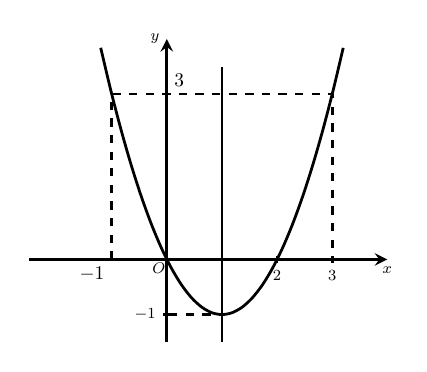
\begin{tikzpicture}[line width=1.0pt,line join=round,>=stealth,scale=0.7,transform shape]
				\draw[->] (-2.5,0) -- (4,0) node[below] {\footnotesize $x$};
				\foreach \x in {2,3}
				\draw[shift={(\x,0)},color=black] (0pt,2pt) -- (0pt,-2pt) node[below] {\footnotesize $\x$};
				\draw[->] (0,-1.5) -- (0,4) node[left] {\footnotesize $y$};
				\foreach \y in {-1}
				\draw[shift={(0,\y)},color=black] (2pt,0pt) -- (-2pt,0pt) node[left] {\footnotesize $\y$}; 
				\draw[color=black] (3pt,2pt) node[below left] {\footnotesize $O$};
				%\clip(-2.4,-1.4) rectangle (3,3.5); 
				\draw[smooth,domain=-1.2:3.2] plot(\x,{(\x)^2-2*(\x)});
				\draw[dashed] (1,0)--(1,-1)--(0,-1) (-1,0)--(-1,3)--(3,3)--(3,0);
				\draw[smooth](1,-1.5)--(1,3.5);
				\draw (-1,0)node[below left]{$-1$};
				\draw (0,3)node[above right]{$3$};
		\end{tikzpicture}}
	}
\end{vd}
\begin{vd}%[Nguyễn Vương Hiển]%[0D2B3-3]
Lập bảng biến thiên và vẽ đồ thị của hàm số $y=-\dfrac{1}{2}x^2+2x-2$.
	\loigiai{
		Ta có $a=-\dfrac{1}{2}, b=2, c=-2$. Suy ra tọa độ đỉnh là $I\left(2;0\right)$.\\
		Vậy bảng biến thiên là
		\begin{center}
			
\begin{tikzpicture}
				\tkzTabInit[nocadre=false, lgt=1, espcl=3]{$x$ /1,$y$ /2}{$-\infty$,$2$,$+\infty$}
				\tkzTabVar{-/ $-\infty$ / ,+/$0$, -/ $-\infty$ /}
			\end{tikzpicture}
		\end{center}
		Do đó hàm số đồng biến trên khoảng $\left(-\infty;2\right)$ và nghịch biến trên khoảng $\left(2;+\infty\right)$.\\
		*Vẽ đồ thị: Ta có đỉnh là $I\left(2;0\right)$ và trục đối xứng là $x=2$.\\
		Bảng giá trị
		\begin{center}
			\begin{tabular}{|c|ccccc|}
				\hline
				$x$& $-2$&$0$ &$2$ & $4$&$6$ \\
				\hline 
				$y$ &$-8$&$-2$ & $0$ &$-2$ &$-8$\\
				\hline
			\end{tabular}
		\end{center}
		\immini{Ta có đồ thị của hàm số $y =-\dfrac{1}{2}x^2+2x-2$ là}
		{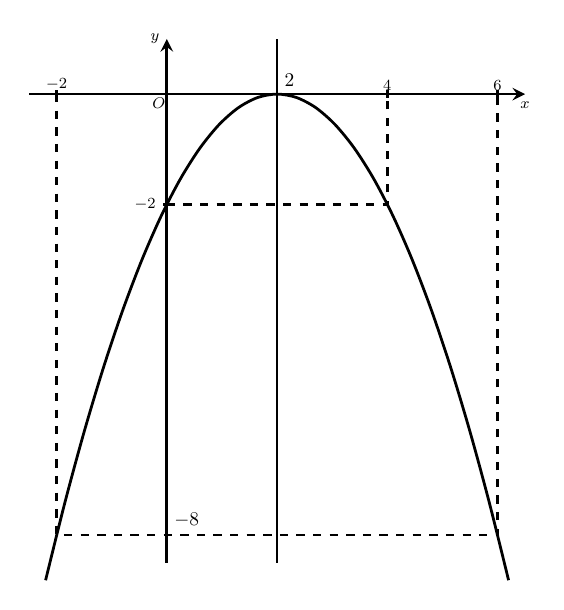
\begin{tikzpicture}[line width=1.0pt,line join=round,>=stealth,scale=0.7,transform shape]
				\draw[->] (-2.5,0) -- (6.5,0) node[below] {\footnotesize $x$};
				\foreach \x in {-2,4,6}
				\draw[shift={(\x,0)},color=black] (0pt,2pt) -- (0pt,-2pt) node[above] {\footnotesize $\x$};
				\draw[->] (0,-8.5) -- (0,1) node[left] {\footnotesize $y$};
				\foreach \y in {-2}
				\draw[shift={(0,\y)},color=black] (2pt,0pt) -- (-2pt,0pt) node[left] {\footnotesize $\y$}; 
				\draw[color=black] (3pt,2pt) node[below left] {\footnotesize $O$};
				%\clip(-2.4,-1.4) rectangle (3,3.5); 
				\draw[smooth,domain=-2.2:6.2] plot(\x,{-0.5*(\x)^2+2*(\x)-2});
				\draw[dashed] (-2,0)--(-2,-8)--(6,-8)--(6,0) (0,-2)--(4,-2)--(4,0);
				\draw (2,-8.5)--(2,1);
				\draw(2,0)node[above right]{$2$};
				\draw(0,-8)node[above right]{$-8$};
		\end{tikzpicture}}
	}
\end{vd}
\begin{dang}{Bài toán tương giao}
	\begin{itemize}
		\item Dựa vào các công thức cần nhớ để tìm tọa độ của đỉnh, giao điểm của parabol với các trục tọa độ. Tuy nhiên, khi tìm tọa độ của đỉnh $I$ thì ta chỉ cần tìm hoành độ $x_0 =-\dfrac{b}{2a}$. Rồi sau đó thế $x_0$ vào hàm số ban đầu để tìm $y_0=a{x_0}^2 + bx_0 + c$ là tung độ của đỉnh $I$.
		\item Dựa vào phương trình hoành độ giao điểm để xác định giao điểm của parabol $(P)$ với đường thẳng.
	\end{itemize}
\end{dang}
\begin{vd}%[Nguyễn Vương Hiển]%[0D2Y3-4]
	Cho hàm số $y=x^2-4x+3$ có đồ thị là parabol $(P)$. Tìm tọa độ của đỉnh, giao điểm của đồ thị với trục tung và trục hoành.
	\loigiai{
		Từ đề ta có: $a = 1, b=-4, c= 3$. Vậy hoành độ của đỉnh $I$ là: $x_0 = -\dfrac{b}{2a}= - \dfrac{-4}{2\cdot1}=2$.\\
		$\Rightarrow y_0 = 2^2- 4\cdot2 + 3 = -1$. Vậy đỉnh $I(2; -1)$.\\
		Giao điểm của $(P)$ và trục $Oy$:
		Cho $x=0 \Rightarrow y= 3$. Vậy $(P)$ cắt trục $Oy$ tại điểm $A(0;3)$.\\
		Giao điểm của $(P)$ với trục $Ox$: Xét phương trình: $x^2 - 4x + 3 =0 \Leftrightarrow \hoac{x=1\\x=3.}$\\
		 Vậy $(P)$ cắt trục $Ox$ tại hai điểm $B(1;0)$ và $C(3;0)$.
	}
\end{vd}
\begin{vd}%[Nguyễn Vương Hiển]%[0D2Y3-4]
	Cho hàm số $y=-x^2-3x+1$ có đồ thị là parabol $(P)$. Tìm tọa độ của đỉnh, giao điểm của đồ thị với trục tung và trục hoành.
	\loigiai{
		Từ đề ta có: $a = -1, b=-3, c= 1$. Vậy hoành độ của đỉnh $I$ là: $x_0 = -\dfrac{b}{2a}= - \dfrac{-3}{-2\cdot1}= -\dfrac{3}{2}$.\\
		$\Rightarrow y_0 = -\left(-\dfrac{3}{2}\right)^2- 3\cdot\left(-\dfrac{3}{2}\right) + 1 = \dfrac{13}{4}$. Vậy đỉnh $I\left(-\dfrac{3}{2};\dfrac{13}{4}\right)$.\\
		Giao điểm của $(P)$ và trục $Oy$:
		Cho $x=0 \Rightarrow y= 1$. Vậy $(P)$ cắt trục $Oy$ tại điểm $A(0;1)$.\\
		Giao điểm của $(P)$ với trục $Ox$: Xét phương trình: $-x^2 - 3x + 1 =0 \Leftrightarrow \hoac{x=\dfrac{-3+\sqrt{13}}{2}\\x=\dfrac{-3-\sqrt{13}}{2}}$.\\
		 Vậy $(P)$ cắt trục $Ox$ tại hai điểm $B\left( \dfrac{-3+\sqrt{13}}{2};0\right)$ và $C\left( \dfrac{-3-\sqrt{13}}{2};0\right)$.
	}
\end{vd}
\begin{dang}{Bài toán thực tế liên quan đến hàm số bậc hai}
% \begin{itemize}
	% \item Phương trình chuyển động của vật chuyển động thẳng biến đổi đều
	% $$y=x_0+v_0t+\dfrac{at^2}{2}$$
	% Trong đó $x_0$ là tọa độ ban đầu của vật, $v_o$ là vận tốc ban đầu của vật và $a$ là gia tốc của vật ($a$ cùng dấu với $v_0$ nếu vật chuyển động nhanh dần đều và ngược dấu với $v_0$ nếu vật chuyển động chậm dần đều). Như vậy toạ độ $x(t)$ của vật là một hàm số bậc hai của thời gian $t$.\\
	% Nói riêng, khi bỏ qua sức cản của không khí, nếu ném một vật lên trên theo phương thẳng đứng thì chuyển động của vật sẽ chỉ chịu ảnh hưởng của trọng lực và vật sẽ có gia tốc bằng gia tốc trọng trường. Khi đó độ cao (so với mặt đất) của vật tại thời điểm $t$ cho bởi phương trình
	% $$y(t)=y_0+v_0\cdot t-\dfrac{1}{2}g\cdot t^2$$
	% Trong đó $y_0$ (mét) là độ cao ban đầu của vật khi ném lên, $v_0$ (m/s) là vận tốc ban đầu của vật và $g$ là gia tốc trọng trường $g\approx 9{,}8$ m/s$^2$.\\
	% Đặc biệt, khi bỏ qua sức cản không khí, nếu một vật rơi tự do từ độ cao $y_0$ (mét) so với mặt đất thì độ cao $y$ (mét) của nó tại thời điểm $t$ (giây) cho bởi công thức
	% $$y(t)=h_{0}-\dfrac{1}{2} g t^{2}.$$
	% \item Phương trình chuyển động của vật ném xiên\\
	% Một vật được ném từ độ cao $h$ (mét) so với mặt đất, với vận tốc ban đầu $v_0$(m/s) hợp với phương ngang một góc $\alpha$. Khi đó quỹ đạo chuyển động của vật tuân theo phương trình
	% $$y=\dfrac{-g}{2 v_{0}^{2} \cos ^{2} \alpha} x^{2}+x \tan \alpha+h$$
	% ở đó $x$ (mét) là khoảng cách vật bay được theo phương ngang tính từ mặt đất tại điểm ném, $y$ (mét) là độ cao so với mặt đất của vật trong quá trình bay, $g$ là gia tốc trọng trường. Như vậy quỹ đạo chuyển động của một vật ném xiên là một parabol.
	% \item Doanh thu bán hàng\\
	% Trong kinh tế, doanh thu bán hàng là số tiền nhận được khi bán một mặt hàng. Doanh thu $R$ bằng đơn giá $x$ của mặt hàng (tức là giá bán của một sản phẩm) nhân với số lượng $n$ sản phẩm đã bán được, tức là
	% $$R=x\cdot n.$$
	% Định luật nhu cầu khẳng định rằng giữa $x$ và $n$ có mối liên hệ với nhau: Khi cái này tăng thì cái kia sẽ giảm. Phương trình liên hệ giữa $x$ và $n$ gọi là phương trình nhu cầu. Nếu phương trình nhu cầu là liên hệ bậc nhất, tức là $n=a-b x$ ( $a, b$ là những hằng số dương) thì doanh thu bán hàng sẽ là hàm số bậc hai của đơn giá
	% $$R(x)=x\cdot n=x(a-b x)=a x-b x^{2}.$$
	% Khi đó người ta thường quan tâm đến việc tìm giá bán $x$ để doanh thu đạt cực đại, hoặc tìm giá bán $x$ để doanh thu vượt một mức nào đó.
% \end{itemize}
\end{dang}
\begin{vd}%[Nguyễn Vương Hiển]%[0D2B3-5]
	Một viên bi rơi tự do từ độ cao $19{,}6$ m xuống mặt đất. Độ cao $h$ (mét) so với mặt đất của viên bi trong khi rơi phụ thuộc vào thời gian $t$ (giây) theo công thức $h=19{,}6-4{,}9t^2$,\quad $h,t\ge0$. Hỏi sau bao nhiêu giây kể từ khi rơi viên bi chạm đất?
	\loigiai{
		Viên bi chạm đất ta có $h=0$.
		$$19{,}6-4{,}9t^2=0\Leftrightarrow\hoac{&t=2\\&t=-2}\Leftrightarrow t=2.$$
		Vậy sau thời gian $t=2$ s thì viên bi chạm đất.
	}
\end{vd}
\begin{vd}%[Nguyễn Vương Hiển]%[0D2K3-5]
	Cổng Arch tại thành phố St Louis của Mỹ có hình dạng là một parabol (hình vẽ). Biết khoảng cách giữa hai chân cổng bằng $162m$. Trên thành cổng, tại vị trí có độ cao $43m$ so với mặt đất (điểm $M$), người ta thả một sợi dây chạm đất (dây căng theo phương vuông góc với đất). Vị trí chạm đất của đầu sợi dây này cách cổng $A$ một đoạn $10m$. Giả sử các số liệu trên là chính xác. Hãy xác tính độ cao của cổng Arch (tính từ mặt đất đến điểm cao nhất của cổng).
	\begin{center}
		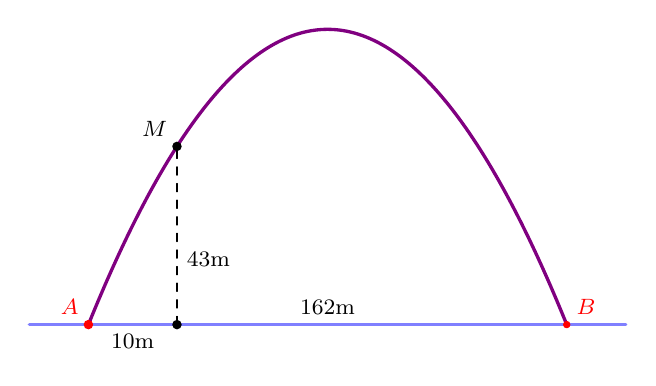
\begin{tikzpicture}[scale=0.75, font=\footnotesize, line join=round, line cap=round, >=stealth]
			\def\xmin{0}\def\xmax{8.1}\def\ymin{-1}\def\ymax{5}\def\scale{20}
			\draw[smooth, very thick, color = violet,samples=200,domain=\xmin:\xmax] plot (\x,{-0.30482*((\x)^2)+2.46913*\x+0});
			\draw[very thick, color = blue!50] (\xmin-1,0) -- (\xmax+1,0);
			\filldraw[color=red] (0,0) circle (2pt) node [above left] {$A$};
			\filldraw[color=red] (162/\scale,0) circle (1.5pt) node [above right] {$B$};
			\foreach \y in {0,3.01785}{
				\filldraw[color=black] (30/\scale,\y) circle (2pt);
			}
			\node[above left] at (30/\scale,3.01785) {$M$};
			\draw[dashed] (30/\scale,0) -- (30/\scale,3.01785);
			\node[right] at (30/\scale,22/\scale) {$43$m};
			\node[above] at (81/\scale,0) {$162$m};
			\node[below] at (15/\scale,0) {$10$m};
		\end{tikzpicture}
	\end{center}
	\loigiai{
		Chọn hệ trục $Oxy$ như hình vẽ
		\begin{center}
			\begin{tikzpicture}[scale=1, font=\footnotesize, line join=round, line cap=round, >=stealth]
				\def\xmin{-1}\def\xmax{5}\def\ymin{-1}\def\ymax{4.5}
				\draw[->] (\xmin-0.2,0)--(\xmax+0.2,0) node[below] {\footnotesize $x$};
				\draw[->] (0,\ymin-0.2)--(0,\ymax+0.2) node[right] {\footnotesize $y$};
				\draw (0,0) circle (1pt) node [below left] {$A$};
				\draw (4.0,0) circle (1pt) node [below right] {$B$};
				\clip (\xmin,\ymin) rectangle (\xmax,\ymax);
				\draw[smooth,samples=200,domain=\xmin:\xmax] plot (\x,{-1*((\x)^2)+4*\x+0});
				\draw[dashed] (1.0,0)--(1.0,3.0)--(0,3.0);\fill (1.0,3.0) circle (1pt) node[above left]{$M$};
				\draw (0,3.0) node[left]{$43$};
				\draw (1.0,0) node[below]{$10$};
				\draw (4.0,0) node[above right]{$162$};
			\end{tikzpicture}
		\end{center}
		Phương trình parabol $(P)$ có dạng $y=ax^2+bx+c$.\\
		Phương trình $(P)$ đi qua ba điểm $A(0;0)$, $B(162;0)$, $M(10;43)$ nên ta có\\ $\heva{&c=0\\&162^2a+162b+c=0\\&10^2a+10b+c=43} \Leftrightarrow \heva{&a=-\dfrac{43}{1520}\\&b=\dfrac{3483}{760}\\&c=0} \Rightarrow (P) \colon y=-\dfrac{43}{1520}x^2+\dfrac{3483}{760}$\\
		Do đó chiều cao của cổng là $h=-\dfrac{\Delta}{4a}=\dfrac{b^2-4ac}{4a} \approx 185,6m$.
	}
\end{vd}
\subsection{Bài tập tự luận}
\subsubsection{Tập xác định, bảng biến thiên, tính đơn điệu, GTLN-GTNN}
\begin{bt}%[0D2B3-1]
	Lập bảng biến thiên của hàm số $y=x^2+6x+5$.
	\loigiai{
		Tập xác định $\mathscr{D}=\mathbb{R}$.\\
		Đỉnh $I(-3;-4)$.\\
		Bảng biến thiên
		\begin{center}
			
\begin{tikzpicture}
				\tkzTabInit[nocadre=false,lgt=.7,espcl=2.5,deltacl=0.6]
				{$x$ /.7,$y$ /2}{$-\infty$,$-3$,$+\infty$}
				\tkzTabVar{+/$+\infty$,-/$-4$,+/$+\infty$}
			\end{tikzpicture}
		\end{center}
		Hàm số đồng biến trên khoảng $(-3;+\infty)$ và nghịch biến trên khoảng $(-\infty;-3)$
	}
\end{bt}
\begin{bt}%[0D2B3-1]
	Lập bảng biến thiên của hàm số $y=x^2+4x+3$.	
	\loigiai{
		Hàm số $y=x^2+4x+3$ có đỉnh $I(-2;-1)$ nên có bảng biến thiên như sau
		\begin{center}
			
\begin{tikzpicture}
				\tkzTabInit[nocadre=false,lgt=1.2,espcl=2.5,deltacl=0.6]
				{$x$ /0.6,$y$ /2}
				{$-\infty$,$-2$,$+\infty$}
				\tkzTabVar{+/$+\infty$, -/$-1$,+/$+\infty$}
			\end{tikzpicture}
		\end{center}		
	}	
\end{bt}
% \begin{bt}%[0D2B3-1]
% 	\immini{Cho đồ thị của hàm số bậc hai như hình bên
% 	\begin{enumerate}
% 		\item Tìm tọa độ đỉnh của đồ thị.
% 		\item Tìm khoảng đồng biến và khoảng nghịch biến của hàm số.
% 		\item Tìm giá trị lớn nhất của hàm số
% 		\item Tìm tập xác định của hàm số
% 	\end{enumerate}}{
% \begin{tikzpicture}[scale=1, font=\footnotesize, line join=round, line cap=round, >=stealth]
% 	\draw[->] (-1.1,0)--(5.1,0) node[below left] {$x$};
% 	\draw[->] (0,-3.1)--(0,1.6) node[below left] {$y$};
% 	\draw (0,0) node [below left] {$O$};
% 	\foreach \x in {1,2,3,4}
% 	\draw[thin] (\x,1pt)--(\x,-1pt);
% 	\node at (0,1)[left]{$1$};
% 	\node at (1,0)[below]{$1$};
% 	\foreach \y in {-1,-2,-3,1}
% 	\draw[thin] (1pt,\y)--(-1pt,\y);
% 	\draw[dashed,thin](2,0)--(2,1)--(0,1);
% 	\begin{scope}
% 		\clip (-1,-3) rectangle (5,1.5);
% 		\draw[samples=200,domain=-1:5,smooth,variable=\x] plot (\x,{(-1/2)*((\x)-2)^2+1});
% 	\end{scope}
% \end{tikzpicture}
% }
% \loigiai{
% \begin{enumerate}
% 	\item Tọa độ đỉnh của hàm số là $I(2;1)$.
% 	\item Hàm số đồng biến trên khoảng $(-\infty;2)$ và nghịch biến trên khoảng $(2;+\infty)$.
% 	\item Hàm số có giá trị lớn nhất là $1$, đạt được khi $x=2$.
% 	\item Tập xác định của hàm số là $\mathbb{R}$. Tập giá trị của hàm số là $(-\infty;1]$.
% \end{enumerate}
% }
% \end{bt}
% \begin{bt}%[0D2B3-1]
% 	\immini{Cho đồ thị của hàm số bậc hai như hình bên
% 	\begin{enumerate}
% 		\item Tìm tọa độ đỉnh của đồ thị.
% 		\item Tìm khoảng đồng biến và khoảng nghịch biến của hàm số.
% 		\item Tìm giá trị lớn nhất của hàm số
% 		\item Tìm tập xác định của hàm số
% 	\end{enumerate}}
% {
% 	\begin{tikzpicture}[scale=1, font=\footnotesize, line join=round, line cap=round, >=stealth]
% 		\draw[->] (-2.1,0)--(4.1,0) node[below left] {$x$};
% 		\draw[->] (0,-4.6)--(0,2.1) node[below left] {$y$};
% 		\draw (0,0) node [below left] {$O$};
% 		\foreach \x in {1}
% 		\draw[thin] (\x,1pt)--(\x,-1pt) node [above] {$\x$};
% 		\foreach \y in {1,-4}
% 		\draw[thin] (1pt,\y)--(-1pt,\y) node [left] {$\y$};
% 		\draw[dashed,thin](1,0)--(1,-4)--(0,-4);
% 		\begin{scope}
% 			\clip (-2,-4.5) rectangle (4,2);
% 			\draw[samples=200,domain=-2:4,smooth,variable=\x] plot (\x,{1*(\x)^2+-2*(\x)+-3});
% 		\end{scope}
% 	\end{tikzpicture}
% }
% \loigiai{
% \begin{enumerate}
% 	\item Tọa độ đỉnh của hàm số là $I(1;-4)$.
% 	\item Hàm số đồng biến trên khoảng $(1;+\infty)$ và nghịch biến trên khoảng $(-\infty;1)$.
% 	\item Hàm số có giá trị nhỏ nhất là $-4$, đạt được khi $x=1$.
% 	\item Tập xác định của hàm số là $\mathbb{R}$. Tập giá trị của hàm số là $[-4;+\infty)$.
% \end{enumerate}
% }
% \end{bt}
\subsubsection{Xác định hàm số bậc hai}
\begin{bt}%[0D2B3-2]
	Cho hàm số $y=x^2+ax+b$. Tìm các hệ số $a$, $b$ biết đồ thị hàm số đi qua hai điểm $M(-1;0)$ và $N(-2;-1)$.
	\loigiai{
		Do đồ thị hàm số đã cho đi qua hai điểm $M$ và $N$ nên
		\[ \heva{&(-1)^2-a+b=0\\ &(-2)^2-2a+b=-1} \Leftrightarrow \heva{&a=4\\ &b=3.} \] 
	}
\end{bt}
\begin{bt}%[0D2B3-2]
	Xác định Parapol $(P)\colon y=ax^2+bx+c$ biết $(P)$ đi qua ba điểm $A(1;1)$, $B(-3;2)$, $C(2;5)$.
	\loigiai{
		Parapol $(P)$ đi qua ba điểm $A(1;1)$, $B(-3;2)$, $C(2;5)$ nên ta có hệ phương trình
		\begin{center}
			$\heva{&a+b+c=1\\&9a-3b+c=2\\&4a+2b+c=5} \Leftrightarrow \heva{&a=\dfrac{17}{20}\\&b=\dfrac{29}{20}\\&c=\dfrac{13}{10}.}$
		\end{center}
		Vậy $(P)\colon y=\dfrac{17}{20}x^2+\dfrac{29}{20}x-\dfrac{13}{10}$.	
	}
\end{bt}
\begin{bt}%[0D2B3-2]
	Tìm parabol $y=ax^2+bx+3$, biết rằng parabol đó
	\begin{enumerate}
		\item đi qua điểm $P(-3;9)$ và có trục đối xứng $x=-1$;
		\item có đỉnh $I(-2;19)$.
	\end{enumerate}
\loigiai{
\begin{enumerate}
	\item Parabol nhận $x=-1$ làm trục đối xứng nên $-\dfrac{b}{2a}=-1\Leftrightarrow b=2a$.\\
	Điểm $P(-3;9)$ thuộc parabol nên $9a-3b+3=9\Leftrightarrow 3a-b=2$.\\
	Do đó ta có $\heva{&b=2a\\&3a-b=2}\Leftrightarrow \heva{&a=2\\&b=4.}$\\
	Vậy parabol cần tìm là $y=2x^2+4x+3$.
	\item Parabol có đỉnh là $I(-2;19)$ nên ta có $$\heva{&-\dfrac{b}{2a}=-2\\&4a-2b+3=19}\Leftrightarrow \heva{&b=4a\\&2a-b=8}\Leftrightarrow \heva{&a=-4\\&b=-16.}$$
	Vậy parabol cần tìm là $y=-4x^2-16x+3$.
\end{enumerate}
}
\end{bt}
\subsubsection{Đồ thị của hàm số bậc hai}
\begin{bt}%[0D2B3-3]
	Lập bảng biến thiên và vẽ đồ thị của hàm số $y=-x^2+4x-3$.
	\loigiai{
		Ta có $-\dfrac{b}{2a}=2$, $y(2)=1$.\\
		Bảng biến thiên
		\begin{center}
			
\begin{tikzpicture}[>=stealth]
				\tkzTabInit[lgt=1.2,espcl=2]
				{$x$ /0.8, $y$ /2}
				{$-\infty$, $2$, $+\infty$}
				\tkzTabVar{-/ $-\infty$, +/ $1$, -/ $-\infty$}
			\end{tikzpicture}
		\end{center}
		\immini{
			Đồ thị hàm số là parabol có đỉnh là điểm $(2;1)$, trục đối xứng là đường thẳng $x=2$, cắt trục tung tại điểm $(0;-3)$ và cắt trục hoành tại hai điểm $(1;0)$, $(3;0)$.
		}{
			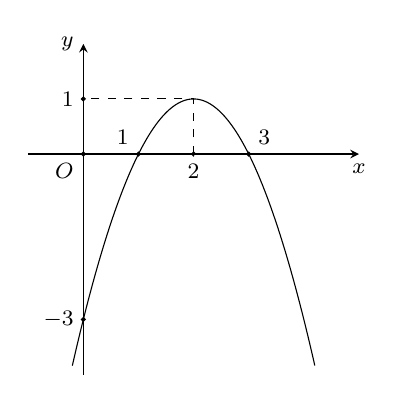
\begin{tikzpicture}[>=stealth,font=\footnotesize,scale=0.7]
				\draw[->] (-1,0) -- (5,0) node[below] {$x$};
				\draw[->] (0,-4) -- (0,2) node[left] {$y$};
				\draw[smooth,samples=100,domain=-0.2:4.2] plot(\x,{-(\x)^2+4*(\x)-3});
				\draw[dashed] (2,0) -- (2,1) -- (0,1);
				\filldraw (0,-3) circle (1pt) node[left] {$-3$};
				\filldraw (0,0) circle (1pt) node[below left] {$O$};
				\filldraw[dashed] (2,0) node[below] {$2$} circle (1pt);
				\filldraw (0,1) circle (1pt) node[left] {$1$};
				\filldraw (1,0) circle (1pt) node[above left] {$1$};
				\filldraw (3,0) circle (1pt) node[above right] {$3$};
			\end{tikzpicture}
		}
	}
\end{bt}
\begin{bt}%[0D2Y3-1]
	Cho hàm số $y = x^2 - 4x + 3$. Lập bảng biến thiên và vẽ đồ thị của hàm số.
	\loigiai
	{ Xét hàm số $y = x^2 - 4x + 3$ có đồ thị là parabol $\left(P\right)$.
		\begin{itemize}
			\item $\left(P\right)$ có tọa độ đỉnh là $I(2;-1)$ và trục đối xứng $x = 2$.
			\item Bảng biến thiên của hàm số
			\begin{center}
				
\begin{tikzpicture}[scale = 1, font=\footnotesize, line join=round, line cap=round, >=stealth]
					\tkzTabInit[lgt=1.2, espcl=2.5, deltacl=0.6]{$x$ /0.6, $y$ /2}{$-\infty$, $2$, $+\infty$}
					\tkzTabVar{+/$+\infty$, -/$-1$, +/$+\infty$}
				\end{tikzpicture}
			\end{center}
			Hàm số đồng biến trên $\left(2;+\infty\right)$ và nghịch biến trên $\left(-\infty;2\right)$.
			\item Đồ thị
			\begin{center}
				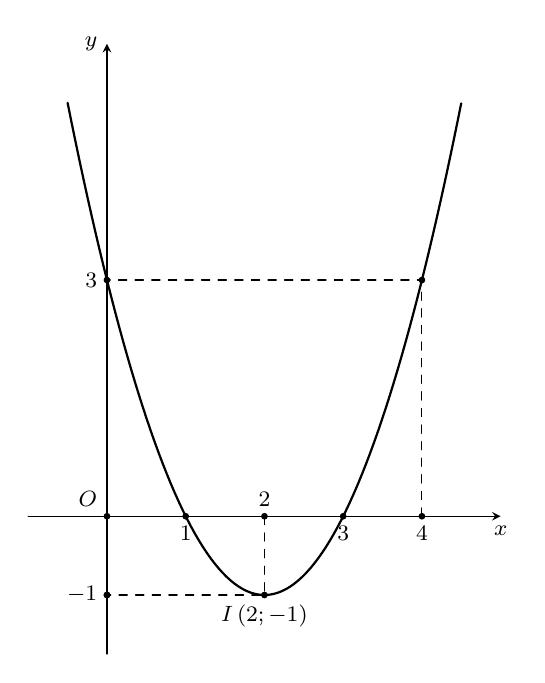
\begin{tikzpicture}[scale = 1, font=\footnotesize, line join=round, line cap=round, >=stealth]
					\draw[->] (-1,0) -- (0,0) node[above left]{$O$} -- (5,0) node[below]{$x$};
					\draw[->] (0,-1.75) -- (0,6) node[left]{$ y $};
					\draw[color = black, thick] plot[domain=-0.5:4.5, samples=100](\x,{(\x)^(2)-4*(\x)+3});
					\draw[fill=black] (1,0) node[below]{$ 1 $} circle (1pt);
					\draw[fill=black] (3,0) node[below]{$ 3 $} circle (1pt);
					\draw[fill=black] (4,0) node[below]{$ 4 $} circle (1pt);
					\draw[fill=black] (0,3) node[left]{$ 3 $} circle (1pt);
					\draw[fill=black] (0,-1) node[left]{$ -1 $} circle (1pt);
					\draw[fill=black] (0,0) circle (1pt) (2,0)node[above]{$2$} circle (1pt) (2,-1) circle (1pt) (0,-1) circle (1pt) (4,3) circle (1pt);
					\draw[dashed] (2,0)--(2,-1)node[below]{$I\left(2;-1\right)$}--(0,-1) (4,0)--(4,3)--(0,3);
				\end{tikzpicture}
			\end{center}
		\end{itemize}
	}
\end{bt}
\begin{bt}%[0D2B3-1]
	\immini{Xác định dấu của các hệ số $a$, $b$, $c$ và dấu của biệt thức $\Delta=b^2-4ac$ của hàm số bậc hai $y=ax^2+bx+c$, biết đồ thị của nó có dạng như hình bên.}{
	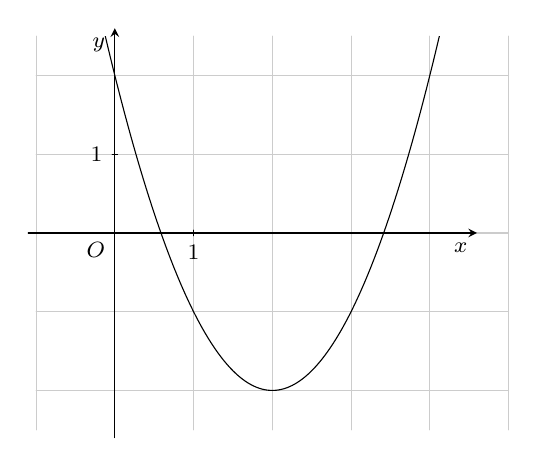
\begin{tikzpicture}[scale=1, font=\footnotesize, line join=round, line cap=round, >=stealth]
		\draw[opacity=.2] (-1,-2.5) grid (5,2.5);
		\draw[->] (-1.1,0)--(4.6,0) node[below left] {$x$};
		\draw[->] (0,-2.6)--(0,2.6) node[below left] {$y$};
		\draw (0,0) node [below left] {$O$};
		\foreach \x in {1}
		\draw[thin] (\x,1pt)--(\x,-1pt) node [below] {$\x$};
		\foreach \y in {1}
		\draw[thin] (1pt,\y)--(-1pt,\y) node [left] {$\y$};
		\begin{scope}
			\clip (-1,-2.5) rectangle (5,2.5);
			\draw[samples=200,domain=-1:5,smooth,variable=\x] plot (\x,{1*(\x)^2+-4*(\x)+2});
		\end{scope}
	\end{tikzpicture}
}
	\loigiai{
	Từ đồ thị của hàm số ta thấy:
	\begin{itemize}
		\item Đồ thị quay bề lõm lên trên nên $a>0$.
		\item Đồ thị cắt trục tung tại điểm có tung độ dương nên $c>0$.
		\item Hoành độ đỉnh $x=-\dfrac{b}{2a}$ có giá trị dương nên $a$ và $b$ trái dấu. Vì $a>0$ nên $b<0$.\\
		Mặt khác, vì đồ thị hàm số cắt trục hoành $Ox$ tại hai điểm phân biệt, tức là phương trình $ax^2+bx+c=0$ có hai nghiệm phân biệt nên $\Delta=b^2-4ac>0$.
	\end{itemize}
	Vậy $a>0$, $b<0$, $c>0$ và $\Delta=b^2-4ac>0$.
}
\end{bt}
\subsubsection{Bài toán tương giao}
\begin{bt}%[0D2B3-4]
	Tìm tọa độ giao điểm của hai đồ thị hàm số $y=x^2-x+1$ {và} $y=2x-1$.
	\loigiai{
		\begin{itemize}
			\item Phương trình hoành độ giao điểm của hai đồ thị là $x^2-3x+2=0$
			$\Leftrightarrow$ $\hoac{&x=1\Rightarrow y= 1\\&x=2\Rightarrow y= 3}$.
			\item Vậy tọa độ giao điểm là: $A(1;1), B(2;3)$.
		\end{itemize}
	}	
\end{bt}
\begin{bt}%[0D2K3-4]
	Tìm tham số $m$ để $(P)\colon y=x^2-2x$ cắt đường thẳng $y=m$ tại hai điểm phân biệt.
	\loigiai{
		Xét phương trình hoành độ giao điểm
		\[x^2-2x=m\Leftrightarrow x^2-2x-m=0.\tag{1}\]
		Ta có $\Delta'=1+m$, $(P)$ cắt đường thẳng $y=m$ tại hai điểm phân biệt khi và chỉ khi (1) có hai nghiệm phân biệt
		$$\Leftrightarrow 1+m>0\Leftrightarrow m>-1.$$
		Vậy $m>-1$.
	}
\end{bt}
\subsubsection{Bài toán thực tế liên quan}
\begin{bt}%[0D2B3-5]
	\immini
	{
		Tháp cầu vượt hai tầng Ngã ba Huế là điểm nhấn kiến trúc mới cho đô thị Đà Nẵng, có hình parabol. Một nhóm học sinh muốn đo chiều cao của tháp bằng cách lập một hệ trục tọa độ sao cho một chân tháp đi qua gốc tọa độ, chân kia của tháp có tọa độ $(30;0)$, và đo được một điểm $M$ trên tháp có tọa độ $(5;34)$. Tính chiều cao của tháp.
	}
	{
		\begin{tikzpicture}[scale=0.1, font=\footnotesize, line join=round, line cap=round, >=stealth]
			\begin{scope}[yscale=0.5]
				\fill[black] (5,34) circle (10pt); 
				\fill[black] (30,0) circle (10pt)+(-90:50 mm) node{$30$};
				\fill[black] (0,0) circle (10pt)+(180:30 mm) node{$O$};
				\draw[->] (0,0)--(35,0) node[below] {\footnotesize $x$};
				\draw[->] (0,0)--(0,306/5+5) node[right] {\footnotesize $y$};
				\draw[dashed] (5,0) node[below]{$5$}|-(0,34)node[left]{$ 34 $}; 
				\draw[samples=100,domain=0:30] plot (\x,{(-34/125)*(\x)^2+(204/25)*(\x)});	
			\end{scope}
		\end{tikzpicture}
	}
	
	\loigiai{
		Giả sử parabol có phương trình $y = ax^2 + bx + c$ $(a \neq 0)$.\\
		Parabol đi qua ba điểm $O(0;0)$; $M(5;34)$ và $N(30;0)$ nên ta có hệ phương trình:
		$$\heva{ & 
			c = 0\\ &
			25a + 5b + c = 34\\ &
			900a + 30b + c = 0
		} \Leftrightarrow \heva{ & 
			a =  - \dfrac{34}{125}\\ &
			b = \dfrac{204}{25}\\ &
			c = 0.
		}$$
		Từ đó, phương trình của parabol là $y =  - \dfrac{34}{125}x^2 + \dfrac{204}{25}{x}$.\\
		Parabol này có đỉnh $I\left(15;\dfrac{306}{5} \right)$, nên tháp có chiều cao $h = \dfrac{306}{5}$.\\
		Vậy chiều cao của tháp là $h = \dfrac{306}{5}$.
	}
\end{bt}
\begin{bt}%[0D2B3-5]
	Một quả bóng cầu thủ sút lên rồi rơi xuống theo quỹ đạo là parabol. Biết rằng ban đầu quả bóng được sút lên từ độ cao $1$ m, sau đó $1$ giây nó đạt độ cao $10$ m và $3{,}5$ giây nó ở độ cao $6{,}25$ m. Hỏi độ cao cao nhất mà quả bóng đạt được là bao nhiêu mét?
	\loigiai{
		\immini
		{
			Biết rằng quỹ đạo của quả bóng là một cung parabol nên phương trình có dạng\\
			$(P)\colon y=ax^2+bx+c$.\\
			Chọn hệ tọa độ như hình vẽ. Với các điểm $A(0;1)$, $B(1;10)$, $C(3{,}5;6{,}25)$, ta có
			$$\heva{&A\left(0;1\right)\in\left(P\right)\\
				&B\left(1;10\right)\in\left(P\right)\\
				&C\left(3,5;6,25\right)\in\left(P\right)}\Leftrightarrow\heva{&c=1\\&a+b+c=10\\&12{,}25a+3{,}5b+c=6{,}25}\Leftrightarrow\heva{&a=-3\\& b=12\\& c=1.}$$
			Suy ra phương trình parabol là $y=-3x^2+12x+1$.\\
			Parabol có đỉnh $I(2;13)$. Khi đó quả bóng đạt vị trí cao nhất tại đỉnh tức $h=13$ m.
		}
		{
			
			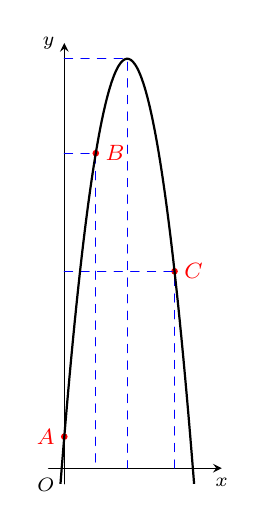
\begin{tikzpicture}[scale=0.4, font=\footnotesize, line join=round, line cap=round, >=stealth]
				\def\a{-3}% Hệ số a phải khác 0
				\def\b{12}
				\def\c{1}
				%\draw[color=gray,dash pattern=on 1pt off 1pt,xstep=1.0cm,ystep=1.0cm](-0.5,-.5)grid(5,13.5);
				\draw[->](-0.5,0)--(5,0)node[below]{\scriptsize $x$};
				\draw[->](0,-0.5)--(0,13.5)node[left]{\scriptsize $y$};
				\draw(0,0)node[below left]{\scriptsize $O$};
				\pgfmathsetmacro\xdinh{-(\b)/2*(\a)}
				\pgfmathsetmacro\ydinh{(4*(\a)*(\c)-(\b)^2)/(4*(\a))}
				%\fill[dashed](\xdinh,\ydinh)circle(2pt)edge(\xdinh,0)edge(0,\ydinh);
				%\draw[dashed,blue] (2,0)-|(0,13);
				\fill[red] (0,1) circle (3pt) node[left]{$A$};
				\fill[red] (1,10) circle (3pt) node[right]{$B$};
				\fill[red] (3.5,6.25) circle (3pt) node[right]{$C$};
				\clip(-0.5,-.5)rectangle(5,13.5);
				\draw[dashed,blue] (0,13)-|(2,0) (0,6.25)-|(3.5,0) (0,10)-|(1,0);
				\draw[thick,samples=150,smooth,domain=-5:5]plot(\x,{\a*(\x)^2+(\b)*\x+(\c)});
			\end{tikzpicture}
		}
	}
\end{bt}
\begin{bt}%[0D2B3-5]
	Một rạp chiếu phim có sức chứa $1\ 000$ người. Với giá vé là $40\ 000$ đồng, trung bình sẽ có khoảng $300$ người đến rạp xem phim mỗi ngày. Để tăng số lượng vé bán ra, rạp chiếu phim đã khảo sát thị trường và thấy rằng nếu giá vé cứ giảm $10\ 000$ đồng thì sẽ có thêm $100$ người đến rạp mỗi ngày.
	\begin{enumerate}
		\item Tìm công thức của hàm số $R(x)$ mô tả doanh thu từ tiền bán vé mỗi ngày của rạp chiếu phim khi giá vé là $x$ nghìn đồng.
		\item Tìm mức giá vé để doanh thu từ tiền bán vé mỗi ngày của rạp là lớn nhất
	\end{enumerate}
\loigiai{
\begin{enumerate}
	\item Khi giá vé là $x$ (nghìn đồng) thì số tiền giảm giá mỗi vé so với mức giá cũ là $40-x$ (nghìn đồng).\\
	Số người tăng lên sau khi giảm giá vé là $\dfrac{100(40-x)}{10}=10(40-x)$.\\
	Số người đến rạp chiếu phim mỗi ngày sau khi giảm giá là 
	$$300+10(40-x)=700-10x.$$
	Công thức của hàm số $R(x)$ mô tả doanh thu từ tiền bán vé mỗi ngày khi giá vé là $x$ (nghìn đồng) là
	$$R(x)=x(700-10x)=-10x^2+700x \text{ (nghìn đồng).}$$
	\item Hàm số $R(x)=-10x^2+700x$ đạt giá trị lớn nhất tại $x-35$. Khi đó
	$$R(35)=12\ 250.$$
	Vậy doanh thu lớn nhất mà rạp chiếu có thể thu được mỗi ngày là $12\ 250\ 000$ đồng khi giá bán mỗi vé là $35\ 000$ đồng.
\end{enumerate}
}
\end{bt}
\begin{bt}%[0D2B3-5]
	Một hòn đá được ném lên trên theo phương thẳng đứng. Khi bỏ qua sức cản không khí, chuyển động của hòn đá tuân theo phương trình sau
	$$y=-4{,}9t^2+mt+n,$$
	với $m$, $n$ là các hằng số. Ở đây $t=0$ là thời điểm hòn đá được ném lên, $y(t)$ là độ cao của hòn đá tại thời điểm $t$ (giây) sau khi ném và $y=0$ ứng với bóng chạm đất.
	\begin{enumerate}
		\item Tìm phương trình chuyển động của hòn đá, biết rằng điểm ném cách mặt đất $1{,}5$ m và thời gian để hòn đá đạt độ cao lớn nhất là $1{,}2$ giây sau khi ném.
		\item Tìm độ cao của hòn đá sau $2$ giây kể từ khi bắt đầu ném.
		\item Sau bao lâu kể từ khi ném, hòn đá rơi xuống mặt đất (Kết quả làm tròn đến chữ số thập phân thứ hai)?
	\end{enumerate}
\loigiai{
\begin{enumerate}
	\item Theo giả thiết điểm ném ở độ cao $1{,}5$ m so với mặt đất nên $n=1{,}5$.\\
	Hòn đá đạt độ cao lớn nhất khi $t=-\dfrac{m}{2\cdot (-4{,}9)}=\dfrac{m}{9{,}8}$.\\
	Theo đề bài ta có $\dfrac{m}{9{,}8}=1{,}2\Leftrightarrow m=11{,}76$.\\
	Vậy phương trình chuyển động của hòn đá là $y=-4{,}9t^2+11{,}76t+1{,}5$.
	\item Khi $t=2$ ta có $y=-4{,}9\cdot 2^2+11{,}76\cdot 2+1{,}5=5{,}42$.\\
	Vậy sau $2$ giây, hòn đá có độ cao là $5{,}42$ m.
	\item Hòn đá rơi xuống mặt đất tức là $y=0$. Xét phương trình 
	$$-4{,}9t^2+11{,}76t+1{,}5=0\Leftrightarrow t\approx 2{,}52\text{ hoặc } t\approx -0{,}12\text{ (loại)}.$$
	Vậy sau khoảng $2{,}52$ giây kể từ khi ném thì hòn đá rơi xuống mặt đất.
\end{enumerate}
}
\end{bt}

\subsection{Bài tập trắc nghiệm}
\Opensolutionfile{ansbook}[ans/ansbook-0D2-1-TN]
\Opensolutionfile{ans}[ans/ans-0D2-1-TN]
\begin{ex}%[0D2Y3-2]
	Hàm số nào sau đây là hàm số bậc hai?
	\choice
	{$y=2x+1$}
	{$y=3x-4$}
	{\True $y=x^2-1$}
	{$y=\dfrac{x+2}{x-1}$}
	\loigiai{
		Hàm số bậc hai có dạng: $y=ax^2+bx+c, (a \neq 0)$ nên $y=x^2-1$ là hàm số bậc hai.
	}
\end{ex}
\begin{ex}%[0D2Y3-3]
	\immini{       
		Đồ thị hình bên là của hàm số nào sau đây?
		\choice        
		{$y=-x^2-2x+3$}
		{$y=x^2+2x-2$}
		{$y=2x^2-4x-2$}
		{\True $y=x^2-2x-1$}}
	{
		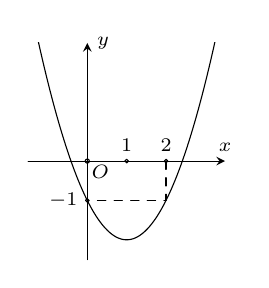
\begin{tikzpicture}[scale=0.5, font=\footnotesize, line join=round, line cap=round, >=stealth]
			\draw[->] (0,-2.5) -- (0,3) node[right]{\scriptsize $y$};
			\draw[->] (-1.5,0) -- (3.5,0) node[above]{\scriptsize $x$};
			\draw (0,0) node[below right=-2pt]{\scriptsize $O$} circle (1.5pt);
			\clip (-1.5,-2.5) rectangle (3.5,3) ; 
			\draw[samples=100,domain=-1.5:3.5] plot (\x,{(\x)^2-2*(\x)-1)});
			\draw (1,0) node[above]{\scriptsize $1$} circle (1.3pt);
			\draw (2,0) node[above]{\scriptsize $2$} circle (1.3pt);
			\draw (0,-1) node[left]{\scriptsize $-1$} circle (1.3pt);
			\draw[dashed] (2,0)--(2,-1)--(0,-1);
	\end{tikzpicture}}
	\loigiai{
		Đồ thị hàm số  cắt trục tung tại điểm $(0;-1)$ suy ra hàm số cần tìm là $y=x^2-2x-1$.	
	}
\end{ex}
\begin{ex}%[0D2B3-1]
	Bảng biến thiên bên dưới là của hàm số nào?
	\begin{center}
		
\begin{tikzpicture}
			\tkzTabInit[nocadre=false,lgt=1.2,espcl=2.5,deltacl=0.6]
			{$x$ /0.6,$y$ /2}
			{$-\infty$,$2$,$+\infty$}
			\tkzTabVar{+/$+\infty$,-/$-6$,+/$+\infty$}
			
		\end{tikzpicture}
	\end{center}
	\choice
	{$y=-x^2+4x+2$}
	{\True $y=x^2-4x-2$}
	{$y=x^2-4x+1$}
	{$y=x^2-4x+2$}
	\loigiai{
		Từ bảng biến thiên suy ra hàm số  đạt giá trị nhỏ nhất bằng $-6$ tại $x=2$. \\
		Do đó bảng biến thiên là của hàm số $y=x^2-4x-2$.
	}
\end{ex}
\begin{ex}%[0D2B3-1]
	Tọa độ đỉnh của đồ thị hàm số $y = 2x^2 + 5x -7$ là
	\choice
	{\True $\left(\dfrac{-5}{4}; \dfrac{-81}{8}\right)$}
	{$\left(\dfrac{-5}{4}; \dfrac{-81}{2}\right)$}
	{$\left(\dfrac{-5}{2}; \dfrac{-81}{2}\right)$}
	{$\left(\dfrac{-5}{2}; \dfrac{-81}{4}\right)$}
	\loigiai{Đồ thị của hàm số $y = ax^2 + bx + c$ $(a \neq 0)$ là Parabol có đỉnh $I\left(\dfrac{-b}{2a}; \dfrac{-\Delta}{4a}\right)$. Từ đây, ta có đỉnh của đồ thị hàm số $y = 2x^2 + 5x -7$ là $I\left(\dfrac{-5}{4}; \dfrac{-81}{8}\right)$.
	}
\end{ex}

\begin{ex}%[0D2B3-1]
	Cho hàm số bậc hai $y=ax^2+bx+c$ ($a\ne 0$) có đồ thị $(P)$, tọa độ đỉnh $I$ của nó được xác định bởi công thức nào?
	\choice
	{\True $I\left(-\dfrac{b}{2a};-\dfrac{\Delta}{4a}\right)$}
	{$I\left(-\dfrac{b}{2a};-\dfrac{\Delta}{2a}\right)$}
	{$I\left(-\dfrac{b}{a};-\dfrac{\Delta}{4a}\right)$}
	{$I\left(\dfrac{b}{a};-\dfrac{\Delta}{4a}\right)$}
	\loigiai{Tọa độ đỉnh của parabol $(P)$ là {$I\left(-\dfrac{b}{2a};-\dfrac{\Delta}{4a}\right)$}.
	}
\end{ex}
\begin{ex}%[0D2Y3-1]
	Parabol $y=x^2+5x+6$ có tọa độ đỉnh là
	\choice
	{$\left(5;\dfrac{1}{2}\right)$}
	{$\left(-\dfrac{5}{2};\dfrac{1}{2}\right)$}
	{$\left(\dfrac{5}{2};\dfrac{1}{4}\right)$}
	{\True $\left(-\dfrac{5}{2};-\dfrac{1}{4}\right)$}
	\loigiai{
		Tọa độ đỉnh của parabol là: $\heva{&x=-\dfrac{b}{2a}=-\dfrac{5}{2} \\& y=-\dfrac{\Delta}{4a}=-\dfrac{1}{4}}\Rightarrow I\left(-\dfrac{5}{2};-\dfrac{1}{4}\right)$.}
\end{ex}
\begin{ex}%[0D2Y3-1]
	Hoành độ đỉnh của parabol $(P) \colon y=2x^2-4x+3$ bằng
	\choice
	{$-2$}
	{$2$}
	{$-1$}
	{\True $1$}
	\loigiai{
		Ta có $x_I=-\dfrac{b}{2a}=1$. Vậy hoành độ đỉnh của $(P)$ là $x_I=1$.}
\end{ex}
\begin{ex}%[0D2B3-1]
	Đường thẳng nào sau đây là trục đối xứng của đồ thị hàm số $y=2x^2+8x+5$?
	\choice
	{\True$x=-2$}
	{$x=2$}
	{$x=4$}
	{$x=-4$}
	\loigiai{
		Trục đối xứng của đồ thị hàm số $y=2x^2+8x+5$ là đường thẳng $x=\dfrac{-b}{2a}=\dfrac{-8}{2\cdot2}=-2$.
	}
\end{ex}
\begin{ex}%[0D2B3-1]
	Hàm số $y=x^2+3x+7$ đồng biến trên khoảng nào dưới đây?
	\choice
	{$\left(-\infty;-\dfrac{3}{2}\right)$}
	{\True $\left(-\dfrac{3}{2};+\infty \right)$}
	{$(-\infty;+\infty)$}
	{$(-3;-1)$}
	\loigiai{
		Ta có $-\dfrac{b}{2a}=-\dfrac{3}{2}$. Vì hệ số $a=1>0$ nên hàm số đồng biến trên khoảng $\left(-\dfrac{3}{2};+\infty \right)$.}
\end{ex}

\begin{ex}%[0D2B3-1]
	Cho hàm số $y=-x^2-2x+8$. Mệnh đề nào sau đây là mệnh đề đúng?
	\choice
	{\True Hàm số nghịch biến trên $(2;3)$}
	{Hàm số nghịch biến trên $(-\infty;-1)$}
	{Hàm số đồng biến trên $(-1;+\infty)$}
	{hàm số đồng biến trên $(-4;2)$}
	\loigiai{
		Ta có tọa độ đỉnh $I(-1;9)$.
		\\ 
		Hệ số $a=-1 \Rightarrow$ hàm số đồng biến trên $(-\infty;-1)$ và nghịch biến trên $(-1;+\infty)$.\\ Từ đó suy ra hàm số nghịch biến trên $(2;3)$.}
\end{ex}
\begin{ex}%[0D2B3-1]
	Cho hàm số $y=x^2-2x-1$, mệnh đề nào \textbf{sai}?
	\choice
	{Hàm số đồng biến trên $(1;+\infty)$}
	{Hàm số nghịch biến trên $(-\infty;1)$}
	{Đồ thị hàm số có đỉnh $I(1;-2)$}
	{\True Đồ thị hàm số có trục đối xứng $x=-2$}
	\loigiai{
		Ta có $a=1>0$; $b=-2$; $c=-1$. \\
		Hàm số đồng biến trên $\left(-\dfrac{b}{2a};+\infty \right)$ hay $(1;+\infty)$.\\
		Hàm số nghịch biến trên $\left(-\infty;-\dfrac{b}{2a}\right)$ hay $(-\infty;1)$.\\
		Tọa độ đỉnh $I\left(-\dfrac{b}{2a};-\dfrac{\Delta}{4a}\right)$ hay $I(1;-2)$.\\
		Đồ thị hàm số có trục đối xứng là $x=1$.}
\end{ex}
\begin{ex}%[0D2B3-1]
	Cho hàm số $y=x^2-2x-3$. Khẳng định nào sau đây đúng?
	\choice
	{Hàm số nghịch biến trên khoảng $(-\infty;2)$}
	{Đồ thị hàm số là parabol có đỉnh $I(2;-3)$}
	{\True Hàm số đồng biến trên khoảng $(1;+\infty)$}
	{Đồ thị hàm số cắt trục tung tại $M(3;0)$}
	\loigiai{
		Hàm số có dạng $y=ax^2+bx+c$, với $a=1>0$, nên đồ thị hàm số là parabol có toạ độ đỉnh dạng $I\left(\dfrac{-b}{2a};\dfrac{- \Delta}{4a}\right)$ là $I(1;0)$, suy ra hàm số nghịch biến trên $(-\infty;1)$, đồng biến trên $(1;+\infty)$; đồ thị cắt trục tung tại điểm $N(0;-3)$.}
\end{ex}

\begin{ex}%[0D2B3-1]
	Cho hàm số: $y=x^2-2x-1$, mệnh đề nào sai?
	\choice
	{Hàm số nghịch biến trên $(-\infty;1)$}
	{Đồ thị hàm số có đỉnh $I(1;-2)$}
	{Hàm số đồng biến trên $(1;+\infty)$}
	{\True Đồ thị hàm số có trục đối xứng: $x=-2$}
	\loigiai{
		Ta có bảng biến thiên của hàm số $y=x^2-2x-1$.\\
		Bảng biến thiên
		\begin{center}
			
\begin{tikzpicture}
				\tkzTabInit[lgt=1.2,espcl=3]
				{$x$ /1, $f(x)$ /1}
				{$-\infty$,$1$,$+\infty$}
				\tkzTabVar{+/$+\infty$,-/$-2$,+/$+\infty$}
				
			\end{tikzpicture}
		\end{center}
		Nhìn vào bảng biến thiên ta thấy A, B, C đúng.\\
		Đồ thị hàm số có trục đối xứng $x=1$ nên D sai.}
\end{ex}
\begin{ex}%[0D2B3-1]
	Bảng biến thiên ở dưới là bảng biến thiên của hàm số nào trong các hàm số được cho ở bốn phương án A, B, C, D sau đây?
	\begin{center}
		
\begin{tikzpicture}
			\tkzTabInit[nocadre,lgt=1.5,espcl=5]{$x$/1.2, $y$/2}{$-\infty$, $2$, $+\infty$} 
			\tkzTabVar{+/ $+\infty$, -/ $-5$ , +/ $+\infty$} 
		\end{tikzpicture}
	\end{center}
	\choice
	{$y=-x^2+4x$}
	{$y=-x^2+4x-9$}
	{\True $y=x^2-4x-1$}
	{$y=x^2-4x-5$}
	\loigiai{
		Dựa vào bảng biến thiến ta thấy hệ số $a>0$, do đó loại phương án \lq\lq $y=-x^2+4x$ \rq\rq\ và \lq\lq $y=-x^2+4x-9$ \rq\rq\ .\\
		Xét hàm số $y=x^2-4x-1$.\\
		Tọa độ đỉnh của hàm số trên là $I=\left(-\dfrac{b}{2a};-\dfrac{\Delta}{4a}\right) \Rightarrow I(2;-5)$.
	}
\end{ex}


\begin{ex}%[0D2B3-1]
	Tìm tất cả các giá trị của $b$ để hàm số $y=x^2+2(b+6)x+4$ đồng biến trên khoảng $(6;+\infty).$
	\choice
	{$b \geq 0$}
	{$b=-12$}
	{\True $b \geq -12$}
	{$b \geq -9$}
	\loigiai{
		Vì hệ số $a=1>0$ và hoành độ đỉnh của parabol là $x=-(b+6)$ nên hàm số đồng biến trên khoảng $(-b-6;+\infty)$. Để hàm số đã cho đồng biến trên khoảng $(6;+\infty)$ thì
		$-(b+6) \leq 6 \Leftrightarrow b \geq -12$.}
\end{ex}
\begin{ex}%[0D2B3-1]
	Cho hàm số $y=-x^2+4x+5$. Khẳng định nào sau đây đúng?
	\choice
	{\True $\max \limits_{x \in (0;3)} y=9$}
	{$\min\limits_{x \in (0;3)} y=8$}
	{$\max \limits_{x \in (0;3)} y=8$}
	{$\min\limits_{x \in (0;3)} y=5$}
	\loigiai{
		Ta có bảng biến thiên:
		\begin{center}
			
\begin{tikzpicture}
				\tkzTabInit[nocadre=false,lgt=1.2,espcl=2.5,deltacl=0.6]
				{$x$/0.6,$y$/2}
				{$0$,$2$,$3$}
				\tkzTabVar{-/$5$,+/$9$,-/$8$}
			\end{tikzpicture}
		\end{center}
		Từ bảng biến thiên ta thấy $\max \limits_{x \in (0;3)} y=9$.
	}
\end{ex}
\begin{ex}%[0D2B3-1]
	Tìm giá trị lớn nhất $M$ và giá trị nhỏ $m$ nhất của hàm số $y=f(x)=x^2-3x$ trên đoạn $[0;2]$.
	\choice
	{$M=-2$; $m=-\dfrac{9}{4}$}
	{$M=\dfrac{9}{4}$; $m=0$}
	{\True $M=0$; $m=-\dfrac{9}{4}$}
	{$M=2$; $m=-\dfrac{9}{4}$}
	\loigiai{
		Hàm số $y=f(x)=x^2-3x$ có đồ thị là một Parabol, có đỉnh $I\left(\dfrac{3}{2};-\dfrac{9}{4}\right)$.\\
		Do $a=1>0$ nên hàm số trên có bảng biến thiên trên $[0;2]$ như sau
		\begin{center}
			
\begin{tikzpicture}
				\tkzTabInit[nocadre=false,lgt=1.2,espcl=3]
				{$x$ /0.8,$f(x)$ /2.5}
				{$0$,$\tfrac{3}{2}$,$2$}
				\tkzTabVar{+/$0$,-/$-\dfrac{9}{4}$,+/$-2$}
			\end{tikzpicture}
		\end{center}
		Từ bảng biến thiên suy ra $M=0$; $m=-\dfrac{9}{4}$.}
\end{ex}
\begin{ex}%[0D2B3-1]
	Tìm $m$ đề hàm số $y=x^2-2x+2m+3$ có giá trị nhỏ nhất trên đoạn $[2;5]$ bằng $-3$.
	\choice
	{$m=-9$}
	{$m=0$}
	{\True$m=-3$}
	{$m=1$}
	\loigiai{
		Parabol $y=x^2-2x+2m+3$ có $a=1>0$ và đỉnh $I(1;2m+2)$ nên hàm số $y=x^2-2x+2m+3$ đồng biến trên khoảng $(1;+\infty)$.\\
		Do đó giá trị nhỏ nhất của hàm số $y=x^2-2x+2m+3$ trên đoạn $[2;5]$ bằng $y(2)=2m+3=-3 \Rightarrow m=-3$.}
\end{ex}

\begin{ex}%[0D2B3-1]
	Cho hàm số $y=x^2-2(m+1)x+3$ (với $m$ là tham số). Trên đoạn $[-2018;2018]$ có bao nhiêu giá trị nguyên của tham số $m$ để hàm số đã cho nghịch biến trên khoảng $(-\infty;-1)$?
	\choice
	{$2019$}
	{$2018$}
	{$2021$}
	{\True $2020$}
	\loigiai{
		Ta có $a=1>0 \Rightarrow$ hàm số nghịch biến trên khoảng $\left(-\infty;-\dfrac{b}{2a}\right)$.\\
		Để hàm số nghịch biến trên khoảng $(-\infty;-1)$ thì $-1<\dfrac{-b}{2a} \Leftrightarrow -1<\dfrac{2(m+1)}{2} \Leftrightarrow m>-2$. \\
		Mà $m \in [-2018;2018]$ nên $m\in (-2;2018]$, do $m\in \mathbb{Z}$ suy ra $m\in \{-1;0;\cdots;2018\}$.\\
		Do đó có $2020$ giá trị nguyên $m$ thỏa mãn yêu cầu bài toán.}
\end{ex}
\begin{ex}%[0D2K3-1]
	Gọi $S$ là tập hợp tất cả các giá trị của tham số $m$ để hàm số $y=x^2+(m-1)x+2m-1$ đồng biến trên $(-2;+\infty )$. Khi đó tập hợp $(-10;10) \cap S$ là tập hợp nào?
	\choice
	{$(-10;5)$}
	{\True $[ 5;10)$}
	{$(5;10)$}
	{$(-10;5 ]$}
	\loigiai{
		Hàm số có hệ số $a=1>0$ nên hàm số nghịch biến trên khoảng $\left(-\infty;\dfrac{1-m}{2}\right)$ và đồng biến trên khoảng $\left(\dfrac{1-m}{2};+\infty \right)$.\\
		Do đó, để hàm số đồng biến trên $(-2;+\infty )$ thì $\dfrac{1-m}{2} \leq -2 \Leftrightarrow m \geq 5$.\\
		Suy ra $S= [ 5;+\infty )$.\\
		Khi đó tập hợp $(-10;10) \cap S= [ 5;10)$.}
\end{ex}

\begin{ex}%[0D2B3-2]
	Parabol $(P) \colon y=ax^2+bx+1$ đi qua hai điểm $A(1;4)$ và $B(-1;2)$ là
	\choice
	{$y=x^2+2x+1$}
	{\True $y=2x^2+x+1$}
	{$y=-x^2+4x+1$}
	{$y=-2x^2-x+1$}
	\loigiai{
		$(P)$ đi qua $A(1;4)$ và $B(-1;2)$ nên ta có hệ $\heva{&4=a+b+1 \\& 2=a-b+1} \Leftrightarrow \heva{&a+b=3 \\& a-b=1} \Leftrightarrow \heva{&a=2 \\& b=1}$.\\
		Suy ra $(P) \colon y=2x^2+x+1$.}
\end{ex}
\begin{ex}%[0D2B3-2]
	Parabol $y=ax^2+bx+c$ đi qua $A(0;-1)$, $B(1;-1)$, $C(-1;1)$ có phương trình là
	\choice
	{\True $y=x^2-x-1$}
	{$y=x^2+x-1$}
	{$y=x^2+x+1$}
	{$y=x^2-x+1$}
	\loigiai{
		Parabol $y=ax^2+bx+c$ đi qua $A(0;-1)$, $B(1;-1)$, $C(-1;1)$ khi và chỉ khi
		$$\heva{&c=-1 \\& a+b+c=-1 \\& a-b+c=1}\Leftrightarrow \heva{&a=1 \\& b=-1 \\& c=-1.}$$
		Vậy parabol có phương trình là $y=x^2-x-1$.}
\end{ex}
\begin{ex}%[0D2B3-2]
	Parabol $y=ax^2+bx+c$ đi qua $A(0;6)$ và có đỉnh $I(-2;4)$ có phương trình là
	\choice
	{$y=x^2+2x+6$}
	{\True $y=\dfrac{1}{2}x^2+2x+6$}
	{$y=x^2+x+4$}
	{$y=x^2+6x+6$}
	\loigiai{
		Parabol có đỉnh $I(-2;4)$ nên ta có $\heva{&-\dfrac{b}{2a}=-2 \\& 4=a \cdot (-2)^2-b \cdot 2+c}\Leftrightarrow \heva{&4a-b=0 \\& 4a-2b+c=4}\qquad (1)$.\\
		Parabol đi qua $A(0;6)$ nên ta có $c=6$\qquad $(2)$.\\
		Từ $(1)$ và $(2)$ ta có $\heva{&4a-b=0 \\& 4a-2b+6=4}\Leftrightarrow \heva{&a=\dfrac{1}{2} \\& b=2 \\& c=6.}$\\
		Vậy phương trình parabol cần tìm là: $y=\dfrac{1}{2}x^2+2x+6$.}
\end{ex}
\begin{ex}%[0D2B3-2]
	Cho $(P) \colon y=x^2+bx+c$ có đỉnh $I(-1;4)$. Tính $M=2b+c$?
	\choice
	{$M=7$}
	{\True $M=9$}
	{$M=-3$}
	{$M=-4$}
	\loigiai{
		Ta có $x_I=\dfrac{-b}{2a}=-1 \Rightarrow b=2$ \\
		Thay $I(-1;4)$ vào $(P)$ ta được $4=(-1)^2+2(-1)+c \Rightarrow c=5$ \\
		Từ đó $M=2 \cdot 2+5=9$.}
\end{ex}

\begin{ex}%[0D2B3-2]
	Parabol $y=ax^2-4x+c$ nhận $I(-2;-1)$ làm đỉnh, có phương trình là
	\choice
	{$y=x^2-4x-1$}
	{\True $y=-x^2-4x-5$}
	{$y=-x^2-4x-13$}
	{$y=x^2-4x-5$}
	\loigiai{
		$I(-2;-1)$ là đỉnh của parabol $y=ax^2-4x+c \Leftrightarrow \heva{&\dfrac{4}{2a}=-2 \\& a \cdot (-2)^2+4 \cdot 2+c=-1} \Leftrightarrow \heva{&a=-1 \\& c=-5.}$\\
		Vậy parabol cần tìm có phương trình là $y=-x^2-4x-5$.}
\end{ex}
\begin{ex}%[0D2B3-2]
	Cho Parabol $(P)\colon y=(m-1)x^2-2(m-2)x+m-3$. Tìm $m$ để $(P)$ có đỉnh là $S(-1 ;-2)$.
	\choice
	{$\dfrac{1}{3}$}
	{$0$}
	{\True $\dfrac{3}{2}$}
	{$\dfrac{2}{3}$}
	\loigiai{
		Điều kiện $m\ne 1$.\\
		Ta có trục đối xứng của đồ thị hàm số là $x=-1\Leftrightarrow \dfrac{m-2}{m-1}=-1\Rightarrow m=\dfrac{3}{2}$.\\
		Thử lại với $m=\dfrac{3}{2}$ ta có hàm số $y=\dfrac{1}{2}x^2+x-\dfrac{3}{2}$ có tọa độ đỉnh là $S(-1;-2).$
	}
\end{ex}
\begin{ex}%[0D2B3-2]
	Xác định hàm số $ y=ax^2+bx+c $ biết đồ thị hàm số đi qua điểm $ A(-1;-8) $ và có đỉnh $ I(2;1) $.
	\choice
	{\True $y=-x^2+4x-3$}
	{$ y=x^2-4x+3 $}
	{$ y=-x^2-4x-3 $}
	{$ y=x^2-2x-1 $}
	\loigiai{Từ giả thiết, suy ra
		$$ \heva{& -\dfrac{b}{2a}=2 \\ & a-b+c=-8\\&4a+2b+c=1 }\Leftrightarrow \heva{& a=-1 \\ & b=4\\&c=-3.}$$}
\end{ex}
\begin{ex}%[0D2B3-2]
	Cho hàm số $y=ax^2+2x+c$, biết rằng hàm số đạt giá trị nhỏ nhất bằng $1$ tại điểm $x=-1$. Khi đó giá trị của $a$ và $c$ là
	\choice
	{\True $a=1,\,c=2$}
	{$a=1,\,c=-2$}
	{$a=-1,\,c=2$}
	{$a=1,\,c=5$}
	\loigiai{
		Thay $x=-1,\,y=1$ vào phương trình hàm số đã cho ta được $1=a\cdot(-1)^2+2\cdot(-1)+c\Leftrightarrow a+c=3$.\\
		Vì hàm số bậc $2$ có giá trị nhỏ nhất nên $a>0$.\\
		Hàm bậc $2$ đạt giá trị nhỏ nhất tại $x=-\dfrac{b}{2a}=\dfrac{-2}{2a}=-1\Leftrightarrow a=1\Rightarrow c=2$.
	}
\end{ex}
\begin{ex}%[0D2K3-2]
	Biết hàm số $y=ax^2+bx+c ~(a\neq 0)$ đạt giá trị lớn nhất bằng $3$ tại $x=2$ và có đồ thị hàm số đi qua điểm $A(0;-1)$. Tính tổng $S=a+b+c$.
	\choice
	{$S=4$}
	{\True $S=2$}
	{$S=-4$}
	{$S=-1$}
	\loigiai{
		Hàm số $y=ax^2+bx+c ~(a\neq 0)$ đạt giá trị lớn nhất bằng $3$ tại $x=2$ và có đồ thị hàm số đi qua điểm $A(0;-1)$ nên ta có:\\
		$$\heva{&a<0\\&\dfrac{-b}{2a}=2\\&4a+2b+c=3\\&c=-1} \Leftrightarrow \heva{&a<0\\&c=-1\\&a=-1\\&b=4\\} .$$
		Vậy $S=a+b+c=2$.
		
	}
\end{ex}
\begin{ex}%[0D2B3-2]
	Biết rằng parabol $(P)\colon y=ax^2-bx+c$ cắt trục tung tại điểm có tung độ là $4$, đi qua điểm $A(3;7)$ và có trục đối xứng là đường thẳng $x=2$. Giá trị của biểu thức $S=abc$ là
	\choice
	{$S=8$}
	{$S=-16$}
	{$S=-8$}
	{\True $S=16$}
	\loigiai{
		\begin{itemize}
			\item Parabol cắt trục tung tại điểm có tung độ là $4$ nên $c=4.$
			\item Parabol đi qua điểm $A(3;7)$ nên có phương trình $9a-3b+c=7.$
			\item Parabol có trục đối xứng là đường thẳng $x=2$ nên $\dfrac{b}{2a}=2.$
			\item Ta được hệ phương trình $\heva{&9a-3b+c=7\\&b=4a\\&c=4}\Leftrightarrow \heva{&a=-1\\&b=-4\\&c=4.}$\\
			Vậy $S=abc=16.$
		\end{itemize}	
	}
\end{ex}
\begin{ex}%[0D2B3-2]
	Xác định parabol $(P)\colon y=ax^2+bx+c$, biết rằng $(P)$ có đỉnh $I(2;-1)$ và cắt trục tung tại điểm có tung độ bằng $-3$.
	\choice
	{$y=x^2-2x-3$}
	{$y=-x^2-2x-3$}
	{\True $y=-\dfrac{1}{2}x^2+2x-3$}
	{$y=\dfrac{1}{2}x^2-2x-3$}
	\loigiai{
		$(P)$ cắt trục tung tại điểm có tung độ bằng $-3$, suy ra $c=-3$.\quad $(1)$\\
		$(P)$ có đỉnh $I(2;-1)$, suy ra $\heva{&-1=4a+2b+c\\ & -\dfrac{b}{2a}=2.}$\quad $(2)$\\
		Từ $(1)$ và hệ $(2)$, ta tìm được $a=-\dfrac{1}{2}$, $ b=2$, $c=-3$.\\
		Vậy $(P)\colon y=-\dfrac{1}{2}x^2+2x-3$.
	}
\end{ex}
\begin{ex}%[0D2K3-2]
	Xác định parabol $y=ax^2+bx+c$ ($a\neq 0$), biết rằng đỉnh của parabol đó có tung độ bằng $-25$, đồng thời parabol đó cắt trục hoành tại hai điểm $A(-4;0)$ và $B(6;0)$.
	\loigiai{
		Vì parabol đó cắt trục hoành tại hai điểm $A(-4;0)$ và $B(6;0)$ nên trục đối xứng của nó có phương trình là $x=1$. Do đó parabol có đỉnh $I(1;-25)$. Từ đó ta có hệ phương trình
		$$\heva{&16a-4b+c=0\\ &36a+6b+c=0\\ &a+b+c=-25}\Leftrightarrow \heva{&a=1\\ &b=-2\\&c=-24.}$$
		Vậy parabol có phương trình $y=x^2-2x-24$.
	}
\end{ex}
\begin{ex}%[0D2K3-2]
	Cho các số nguyên $a$, $c$ sao cho parabol $y=ax^2-4x+c$ đi qua điểm $M(4;2)$ và có tung độ đỉnh là $-2$. Tính tổng $S=a+c$.
	\choice
	{\True $S=3$}
	{$S=4$}
	{$S=-1$}
	{$S=1$}
	\loigiai{
		Parabol $P$ đi qua điểm $M(4;2)$ nên ta có $2=16a-16+c \Leftrightarrow c=18-16a$.\\
		Tung độ đỉnh là $-2$ nên $-16+4ac=-2.4a \Leftrightarrow  -16 +4a (18-16a) +8a =0 \Leftrightarrow 4a^2 -5a+1=0 \Leftrightarrow a =1$ hoặc $a=\dfrac{1}{4}$ (loại)\\
		Với $a=1$ suy ra $c=2$. Vậy $S=a+c =3$.
	}
\end{ex}
\begin{ex}%[0D2B3-2]
	Tìm các số thực $a$, $c$ $(c>0)$ sao cho parabol $(P)\colon y=ax^2+2x+c$ đi qua điểm $M(2;3)$ và có tung độ đỉnh là $4$.
	\choice
	{$a=1, c=-5$}
	{$a=-2, c=7$}
	{$a=2, c=-9$}
	{\True $a=-1, c=3$}
	\loigiai{Điểm $M(2;3)\in(P)\Leftrightarrow 3=a\cdot2^2+2\cdot2+c\Leftrightarrow c=-1-4a$\hfill$(1)$.\\
		$(P)$ có tung độ đỉnh bằng $4$ khi và chỉ khi $-\dfrac{\Delta}{4a}=4.$\\
		$\Leftrightarrow \dfrac{-(b^2-4ac)}{4a}=4\Leftrightarrow -(2^2-4ac)=16a\Leftrightarrow ac-1=4a$\hfill$(2)$\\
		Thay $(1)$ vào $(2)$, ta được: $a(-1-4a)-1=4a\Leftrightarrow -4a^2-5a-1=0\Leftrightarrow\hoac{&a=-1\Rightarrow c=3\:(\text{nhận})\\
			&a=-\dfrac{1}{4}\Rightarrow c=0\:(\text{loại})}$}
\end{ex}

\begin{ex}%[0D2K3-2]
	Cho Parabol $(P)\colon y=ax^2+bx+c\,(a, b, c \in \mathbb{Z})$. Biết $(P)$ đi qua điểm $A(1;-1)$,  $B(3;-11)$ và đỉnh của $(P)$ có tung độ bằng $-\dfrac{7}{8}$. Tính $S=a+b-c$.
	\choice
	{\True $S=3$}
	{$S=5$}
	{$S=7$}
	{$S=4$}
	\loigiai{
		Vì $(P)$ đi qua điểm $A(1;-1)$,  $B(3;-11)$ và đỉnh của $(P)$ có tung độ bằng $-\dfrac{7}{8}$, ta có
		\begin{eqnarray*}
			&&\heva{& -1=a+b+c \\ & -11=9a+3b+c\\& -\dfrac{7}{8}=-\dfrac{b^2-4ac}{4a}}
			\Leftrightarrow \heva{& c=-a-b-1 \\& -11=9a+3b-a-b-1\\&7a=2\left[b^2-4a(-a-b-1)\right]}\\
			&\Leftrightarrow& \heva{& c=-a-b-1 \\& 4a+b=-5\\&8a^2+2b^2+8ab+a=0}
			\Leftrightarrow \heva{& c=-a-b-1\\& b=-4a-5\\&8a^2+2(-4a-5)^2+8a(-4a-5)+a=0}\\
			&\Leftrightarrow& \heva{& c=-a-b-1 \\& b=-4a-5\\&8a^2+41a+50=0}
			\Leftrightarrow\heva{& \hoac{& a=-2 \in \mathbb{Z} \\ & a=-\dfrac{25}{8} \notin \mathbb{Z}\text{ (loại)}} \\ & b=3\\&c=-2.}
		\end{eqnarray*}		
		Vậy $S=a+b-c=3$.
	}
\end{ex}
\begin{ex}%[0D2G3-2]
	Cho hàm số $y=x^2-2(m+2)x-m+3$ có đồ thị là parabol $(P)$. Khi $m$ thay đổi, đỉnh $I$ của $(P)$ luôn di chuyển trên một parabol cố định. Phương trình parabol đó là
	\choice
	{$y=x^2-4x+2$}
	{\True $y=-x^2-x+5$}
	{$y=-x^2+4x-3$}
	{$y=-x^2-5x-1$}
	\loigiai{
		Tọa độ đỉnh $I$ của parabol $(P)$ là $\heva{&x_I=m+2\quad(1)\\&y_I=(m+2)^2-2(m+2)^2-m+3\quad(2)}$.\\
		Từ $(1)$ suy ra $m=x_I-2$, thay vào $(2)$ ta có
		\[y_I=x_I^2-2x_I^2-x_I+5\Leftrightarrow y_I=-x_I^2-x_I+5.\]
		Vậy $I$ luôn di chuyển trên parabol cố định có phương trình $y=-x^2-x+5$.
	}
\end{ex}
\begin{ex}%[0D2B3-3]
	\immini{
		Hình vẽ bên là đồ thị của hàm số nào?
		\choice
		{\True $y=-x^2+2x-1$}
		{$y=x^2-2x-1$}
		{$y=-x^2-2x-1$}
		{$y=-x^2+2x+3$}
	}{
		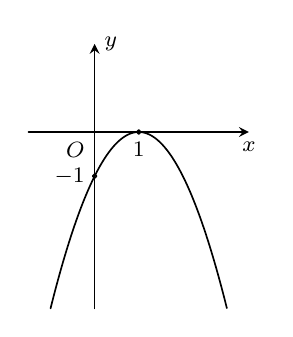
\begin{tikzpicture}[>=stealth,line cap=round,line join=round,scale=.7,font=\footnotesize,line width=.6pt,x=.8cm, y=.8cm]
			\draw[->] (-1.5,0)--(0,0) node[below left]{$O$}--(3.5,0) node[below]{$x$};
			\draw[->] (0,-4) --(0,2) node[right]{$y$};
			\foreach \x in {1}{
				\draw (\x,0) node[below]{$\x$} circle (1pt);
			}
			\foreach \y in {-1}{
				\draw (0,\y) node[left]{$\y$} circle (1pt);
			}
			\draw[smooth,samples=100,domain=-1:3] plot (\x, {-(\x)^2+2*(\x)-1});
		\end{tikzpicture}
	}	
	\loigiai{
		Đồ thị có bề lõm quay xuống, đỉnh $I(1;0)$.\\ 
		Giao của đồ thị với trục tung là $(0;-1)$. Nên đồ thị hàm số cần tìm là $y=-x^2+2x-1$.}
\end{ex}
\begin{ex}%[0D2B3-3]
	\immini{Cho hàm số $y=ax^2+bx+c$ với $(a, b, c \in \mathbb{R}, a \neq 0)$ có đồ thị như hình bên. Đồ thị bên là của hàm số nào?
		\choice
		{\True $y=2x^2-4x-1$}
		{$y=x^2-4x-1$}
		{$y=2x^2-4x+1$}
		{$y=-2x^2-4x-1$}
	}
	{	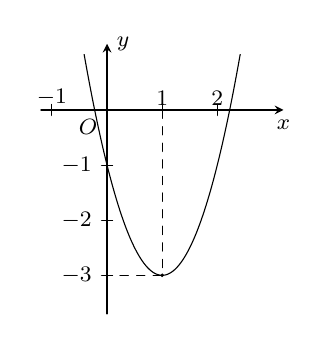
\begin{tikzpicture}[scale=.7, font=\footnotesize, line join=round, line cap=round, >=stealth]
			\def\xmin{-1}\def\xmax{3}\def\ymin{-3.5}\def\ymax{1}
			\draw[->] (\xmin-0.2,0)--(\xmax+0.2,0) node[below] {\footnotesize $x$};
			\draw[->] (0,\ymin-0.2)--(0,\ymax+0.2) node[right] {\footnotesize $y$};
			\draw (0,0) node [below left] {\footnotesize $O$};
			\foreach \x in {-1,1,2}\draw (\x,0.1)--(\x,-0.1) node [above] {\footnotesize $\x$};
			\foreach \y in {-3,-2,-1}\draw (0.1,\y)--(-0.1,\y) node [left] {\footnotesize $\y$};
			\clip (\xmin,\ymin) rectangle (\xmax,\ymax);
			\draw[smooth,samples=200,domain=\xmin:\xmax] plot (\x,{2*((\x)^2)+-4*\x+-1});
			\draw[dashed] (1.0,0)--(1.0,-3.0)--(0,-3.0);\fill (1.0,-3.0) circle (1pt);
		\end{tikzpicture}
	}
	\loigiai{
		Đồ thị hàm số đi qua điểm $(0;-1)$ và có tọa độ đỉnh là $(1;-3)$. Ta có
		$$\heva{&0\cdot a+0\cdot b+c=-1\\&1^2\cdot a+1\cdot b+c=-3\\&-\dfrac{b}{2a}=1}\Leftrightarrow \heva{&c=-1\\&a+b+c=-3\\&2a+b=0}\heva{&a=2\\&b=-4\\&c=-1}\Rightarrow y=2x^2-4x-1.$$
	}
\end{ex}
\begin{ex}%[0D2B3-3]
	\immini{
		Hàm số nào trong 4 phương án liệt kê ở A, B, C, D dưới đây có đồ thị như hình bên?
		\choice
		{$y=-x^2+3x-1$}
		{$y=-2x^2+3x-1$}
		{\True $y=2x^2-3x+1$}
		{$y=x^2-3x+2$}}
	{\begin{tikzpicture}[font=\footnotesize,line join = round, line cap = round,>=stealth,scale=1]
			\draw[->] (-1,0)--(0,0) node[below right]{$O$}--(2.5,0) node[below]{$x$};
			\draw[->] (0,-1)--(0,2.4) node[right]{$y$};
			\draw[samples=100,domain=-0.3:1.8,smooth] plot (\x, {2*(\x)^2-3*(\x)+1});
			\fill[black] (1,0) circle (1.5pt)node [above] {$1$};
			\fill[black] (0,1) circle (1.5pt) node [left] {$1$};
			\fill[black] (0.5,0) circle (1.5pt) ;
	\end{tikzpicture}}
	\loigiai{
		\begin{itemize}
			\item Đồ thị hàm số $y=-x^2+3x-1$ cắt trục tung tại điểm có tọa độ $(0; -1)$ nên không thỏa.
			\item Đồ thị hàm số $y=-2x^2+3x-1$ cắt trục tung tại điểm có tọa độ $(0; -1)$ nên không thỏa.
			\item Đồ thị hàm số $y=x^2-3x+2$ cắt trục tung tại điểm có tọa độ $(0; 2)$ nên không thỏa.
			\item Đồ thị hàm số $y=2x^2-3x+1$ cắt trục tung tại điểm có tọa độ $(0; 1)$ và cắt trục hoành tại hai điểm có tọa độ $\left(\dfrac{1}{2}; 0\right)$ và $(1; 0)$ nên thỏa mãn.
		\end{itemize}
	}
\end{ex}
\begin{ex}%[0D2B3-3]
	Đồ thị hàm số $y=4x^2-3x-1$ có dạng nào trong các dạng sau đây?
	\choice
	{	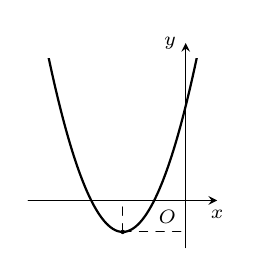
\begin{tikzpicture}[>=stealth,line join=round, line cap=round, font=\footnotesize, scale=.4]
			\def\a{1} % Hệ số a phải khác 0
			\def\b{4}
			\def\c{3}
			\draw[->] (-5,0) -- (1,0) node[below] {\scriptsize $x$};
			\draw[->] (0,-1.5) -- (0,5) node[left] {\scriptsize $y$};
			\draw (0,0)node[below left]{\scriptsize $O$};
			\pgfmathsetmacro\xdinh{-(\b)/2*(\a)}
			\pgfmathsetmacro\ydinh{(4*(\a)*(\c)-(\b)^2)/(4*(\a))}
			\fill[dashed] (\xdinh,\ydinh)circle(2pt) edge (\xdinh,0) edge (0,\ydinh);
			\clip (-5,-1.5)rectangle(1,4.5);
			\draw[thick,samples=150,smooth,domain=-5:5] plot(\x,{\a*(\x)^2+(\b)*\x+(\c)});
		\end{tikzpicture}
	}
	{\True 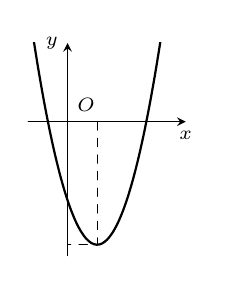
\begin{tikzpicture}[>=stealth,line join=round, line cap=round, font=\footnotesize, scale=1]
			\def\a{4} % Hệ số a phải khác 0
			\def\b{-3}
			\def\c{-1}
			\draw[->] (-.5,0) -- (1.5,0) node[below] {\scriptsize $x$};
			\draw[->] (0,-1.7) -- (0,1) node[left] {\scriptsize $y$};
			\draw (0,0)node[above right]{\scriptsize $O$};
			\draw[dashed] (3/8,0)|-(0,-25/16);
			\clip (-.5,-1.7)rectangle(1.5,1);
			\draw[thick,samples=150,smooth,domain=-5:5] plot(\x,{\a*(\x)^2+(\b)*\x+(\c)});
	\end{tikzpicture}}
	{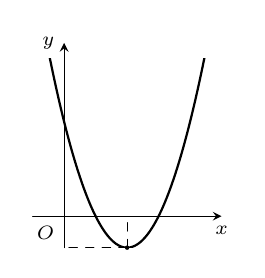
\begin{tikzpicture}[>=stealth,line join=round, line cap=round, font=\footnotesize, scale=.4]
			\def\a{1} % Hệ số a phải khác 0
			\def\b{-4}
			\def\c{3}
			\draw[->] (-1,0) -- (5,0) node[below] {\scriptsize $x$};
			\draw[->] (0,-1) -- (0,5.5) node[left] {\scriptsize $y$};
			\draw (0,0)node[below left]{\scriptsize $O$};
			\pgfmathsetmacro\xdinh{-(\b)/2*(\a)}
			\pgfmathsetmacro\ydinh{(4*(\a)*(\c)-(\b)^2)/(4*(\a))}
			\fill[dashed] (\xdinh,\ydinh)circle(2pt) edge (\xdinh,0) edge (0,\ydinh);
			\clip (-1,-1)rectangle(5,5);
			\draw[thick,samples=150,smooth,domain=-5:5] plot(\x,{\a*(\x)^2+(\b)*\x+(\c)});
	\end{tikzpicture}}
	{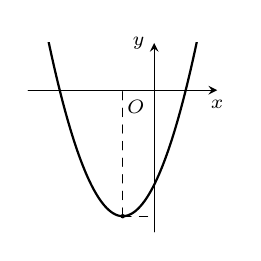
\begin{tikzpicture}[>=stealth,line join=round, line cap=round, font=\footnotesize, scale=.4]
			\def\a{1} % Hệ số a phải khác 0
			\def\b{2}
			\def\c{-3}
			\draw[->] (-4,0) -- (2,0) node[below] {\scriptsize $x$};
			\draw[->] (0,-4.5) -- (0,1.5) node[left] {\scriptsize $y$};
			\draw (0,0)node[below left]{\scriptsize $O$};
			\pgfmathsetmacro\xdinh{-(\b)/2*(\a)}
			\pgfmathsetmacro\ydinh{(4*(\a)*(\c)-(\b)^2)/(4*(\a))}
			\fill[dashed] (\xdinh,\ydinh)circle(2pt) edge (\xdinh,0) edge (0,\ydinh);
			\clip (-4,-4.5)rectangle(2,1.5);
			\draw[thick,samples=150,smooth,domain=-5:5] plot(\x,{\a*(\x)^2+(\b)*\x+(\c)});
		\end{tikzpicture}
	}
	\loigiai{
		Tọa độ đỉnh của Parabol $S\left(\dfrac{3}{8};-\dfrac{25}{16}\right)$.\\
		Trục đối xứng $x=\dfrac{3}{8}>0$.\\
		Đồ thị cắt trục $Oy$ tại điểm $A(0;-1)$.	
	}
\end{ex}

\begin{ex}%[0D2B3-3]
	Cho hàm số $y=ax^2+bx+c$ với $a>0$, $b>0$, $c>0$. Đồ thị của hàm số là hình nào trong các hình dưới đây?
	\begin{center}
		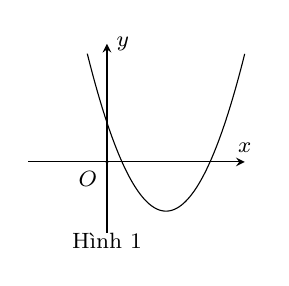
\begin{tikzpicture}[>=stealth,font=\footnotesize,scale=0.5]
			\draw[->](-2,0)--(3.5,0)node[above]{$x$};
			\draw[->](0,-1.8)--(0,3)node[right]{$y$};
			\draw[smooth,samples=100,domain=-0.5:3.5]plot(\x,{(\x)^2-3*\x+1});
			\node at (0,-2) {Hình 1};
			\fill (0,0)node[below left]{$O$}circle (1.2pt);
		\end{tikzpicture}
		\quad
		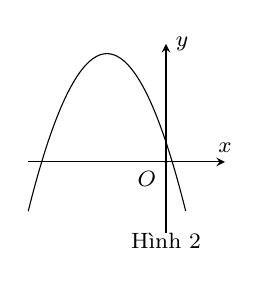
\begin{tikzpicture}[>=stealth,font=\footnotesize,scale=0.5]
			\draw[->](-3.5,0)--(1.5,0)node[above]{$x$};
			\draw[->](0,-1.8)--(0,3)node[right]{$y$};
			\draw[smooth,samples=100,domain=-3.5:0.5]plot(\x,{-1*(\x)^2-3*\x+0.5});
			\node at (0,-2) {Hình 2};
			\fill (0,0)node[below left]{$O$}circle (1.2pt);
		\end{tikzpicture}
		\quad
		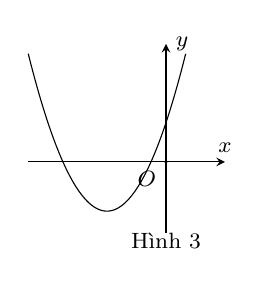
\begin{tikzpicture}[>=stealth,font=\footnotesize,scale=0.5]
			\draw[->](-3.5,0)--(1.5,0)node[above]{$x$};
			\draw[->](0,-1.8)--(0,3)node[right]{$y$};
			\draw[smooth,samples=100,domain=-3.5:0.5]plot(\x,{(\x)^2+3*\x+1});
			\node at (0,-2) {Hình 3};
			\fill (0,0)node[below left]{$O$}circle (1.2pt);
		\end{tikzpicture}
		\quad
		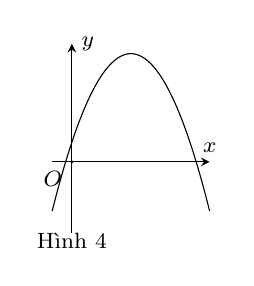
\begin{tikzpicture}[>=stealth,font=\footnotesize,scale=0.5]
			\draw[->](-0.5,0)--(3.5,0)node[above]{$x$};
			\draw[->](0,-1.8)--(0,3)node[right]{$y$};
			\draw[smooth,samples=100,domain=-0.5:3.5]plot(\x,{-1*(\x)^2+3*\x+0.5});
			\node at (0,-2) {Hình 4};
			\fill (0,0)node[below left]{$O$}circle (1.2pt);
		\end{tikzpicture}	
	\end{center}
	\choice
	{Hình $(4)$}
	{\True Hình $(3)$}
	{Hình $(1)$}
	{Hình $(2)$}
	\loigiai{
		Dựa vào hình dáng đồ thị, vì $a>0$ nên loại hình (2) và hình (4).\\
		Vì $b>0$ nên $-\dfrac{b}{a}<0$, do đó đính của parabol nằm bên trái trục tung, do đó chọn hình (3).}
\end{ex}
\begin{ex}%[0D2B3-3]
	Cho hàm số $y=-\dfrac{1}{2}x^2-x+2$ có đồ thị là hình nào dưới đây?
	\choice
	{\True 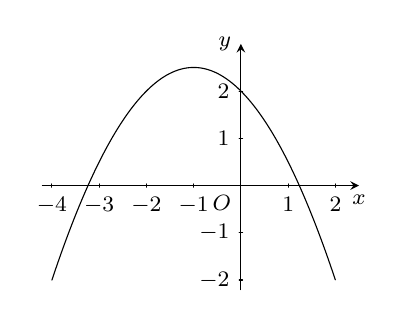
\begin{tikzpicture}[scale=.6, font=\footnotesize,line join=round, line cap=round, >=stealth]
			\draw[->] (-4.2,0)--(0,0) node[below left]{$O$}--(2.5,0) node[below]{$x$};
			\draw[->] (0,-2.2)--(0,3) node[left]{$y$};
			\draw[samples=100,domain=-4:2,smooth] plot (\x, {-0.5*(\x)^2-(\x)+2});
			\foreach \x in {-4,-3,-2,-1,1,2} \draw[thin] (\x,1pt)--(\x,-1pt) node [below] {$\x$};
			\foreach \y in {-2,-1,1,2} \draw[thin] (1pt,\y)--(-1pt,\y) node [left] {$\y$};
	\end{tikzpicture}}
	{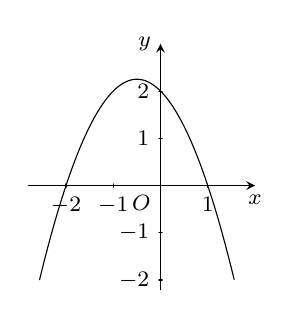
\begin{tikzpicture}[scale=.6, font=\footnotesize,line join=round, line cap=round, >=stealth]
			\draw[->] (-2.8,0)--(0,0) node[below left]{$O$}--(2,0) node[below]{$x$};
			\draw[->] (0,-2.2)--(0,3) node[left]{$y$};
			\draw[samples=100,domain=-2.56:1.56,smooth] plot (\x, {-(\x)^2-(\x)+2});
			\foreach \x in {-2,-1,1} \draw[thin] (\x,1pt)--(\x,-1pt) node [below] {$\x$};
			\foreach \y in {-2,-1,1,2} \draw[thin] (1pt,\y)--(-1pt,\y) node [left] {$\y$};
	\end{tikzpicture}}
	{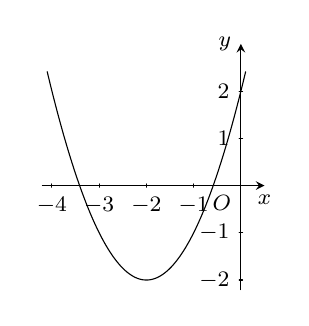
\begin{tikzpicture}[scale=.6, font=\footnotesize,line join=round, line cap=round, >=stealth]
			\draw[->] (-4.2,0)--(0,0) node[below left]{$O$}--(0.5,0) node[below]{$x$};
			\draw[->] (0,-2.2)--(0,3) node[left]{$y$};
			\draw[samples=100,domain=-4.1:0.1,smooth] plot (\x, {(\x)^2+4*(\x)+2});
			\foreach \x in {-4,-3,-2,-1} \draw[thin] (\x,1pt)--(\x,-1pt) node [below] {$\x$};
			\foreach \y in {-2,-1,1,2} \draw[thin] (1pt,\y)--(-1pt,\y) node [left] {$\y$};
	\end{tikzpicture}}
	{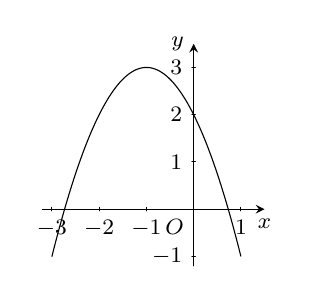
\begin{tikzpicture}[scale=.6, font=\footnotesize,line join=round, line cap=round, >=stealth]
			\draw[->] (-3.2,0)--(0,0) node[below left]{$O$}--(1.5,0) node[below]{$x$};
			\draw[->] (0,-1.2)--(0,3.5) node[left]{$y$};
			\draw[samples=100,domain=-3:1,smooth] plot (\x, {-(\x)^2-2*(\x)+2});
			\foreach \x in {-3,-2,-1,1} \draw[thin] (\x,1pt)--(\x,-1pt) node [below] {$\x$};
			\foreach \y in {-1,1,2,3} \draw[thin] (1pt,\y)--(-1pt,\y) node [left] {$\y$};
	\end{tikzpicture}}
	\loigiai{
		Vì $a=-\dfrac{1}{2}<0$ nên đồ thị quay bề lõm xuống dưới.\\
		Phương trình hoành độ giao điểm $-\dfrac{1}{2}x^2-x+2=0 \Rightarrow \hoac{&x=-1+\sqrt{5} \approx 1{,}23>1 \\& x=-1-\sqrt{5} \approx -3{,}23<-3.}$
	}
\end{ex}
%\begin{ex}%[0D2B3-3]
%	Hàm số $y=-x^2+2x+3$ có đồ thị là hình nào trong các hình sau?
%	\choice
%	{\True \begin{tikzpicture}[line join=round, line cap=round,>=stealth,scale=.6]
%			\def\xmin{-2}\def\xmax{4}\def\ymin{-1}\def\ymax{5}
%			\draw[->] (\xmin-0.2,0)--(\xmax+0.2,0) node[below] {\footnotesize $x$};
%			\draw[->] (0,\ymin-0.2)--(0,\ymax+0.2) node[right] {\footnotesize $y$};
%			\draw (0,0) node [below left] {\footnotesize $O$};
%			\foreach \x in {-2,-1,1,2,3}\draw (\x,0.1)--(\x,-0.1) node [below] {\footnotesize $\x$};
%			\foreach \y in {-1,1,2,3,4}\draw (0.1,\y)--(-0.1,\y) node [left] {\footnotesize $\y$};
%			\clip (\xmin,\ymin) rectangle (\xmax,\ymax);
%			\draw[smooth,samples=200,domain=\xmin:\xmax] plot (\x,{-1*((\x)^2)+2*\x+3});
%			\draw[dashed] (1.0,0)--(1.0,4.0)--(0,4.0);\fill (1.0,4.0) circle (1pt);
%	\end{tikzpicture} }
%	{\begin{tikzpicture}[line join=round, line cap=round,>=stealth,scale=.6]
%			\def\xmin{-4}\def\xmax{2}\def\ymin{-1.5}\def\ymax{4}
%			\draw[->] (\xmin-0.2,0)--(\xmax+0.2,0) node[below] {\footnotesize $x$};
%			\draw[->] (0,\ymin-0.2)--(0,\ymax+0.2) node[right] {\footnotesize $y$};
%			\draw (0,0) node [below left] {\footnotesize $O$};
%			\foreach \x in {-4,-3,-2,-1,1}\draw (\x,0.1)--(\x,-0.1) node [below] {\footnotesize $\x$};
%			\foreach \y in {-1,1,2,3}\draw (0.1,\y)--(-0.1,\y) node [left] {\footnotesize $\y$};
%			\clip (\xmin,\ymin) rectangle (\xmax,\ymax);
%			\draw[smooth,samples=200,domain=\xmin:\xmax] plot (\x,{-1*((\x)^2)+-2*\x+2});
%			\draw[dashed] (-1.0,0)--(-1.0,3.0)--(0,3.0);\fill (-1.0,3.0) circle (1pt);
%	\end{tikzpicture}}
%	{\begin{tikzpicture}[line join=round, line cap=round,>=stealth,scale=.6]
%			\def\xmin{-1}\def\xmax{5.4}\def\ymin{-2}\def\ymax{4}
%			\draw[->] (\xmin-0.2,0)--(\xmax+0.2,0) node[below] {\footnotesize $x$};
%			\draw[->] (0,\ymin-0.2)--(0,\ymax+0.2) node[right] {\footnotesize $y$};
%			\draw (0,0) node [below left] {\footnotesize $O$};
%			\foreach \x in {-1,1,2,3,4,5}\draw (\x,0.1)--(\x,-0.1) node [below] {\footnotesize $\x$};
%			\foreach \y in {-2,-1,1,2,3}\draw (0.1,\y)--(-0.1,\y) node [left] {\footnotesize $\y$};
%			\clip (\xmin,\ymin) rectangle (\xmax,\ymax);
%			\draw[smooth,samples=200,domain=\xmin:\xmax] plot (\x,{1*((\x)^2)+-4*\x+3});
%			\draw[dashed] (2.0,0)--(2.0,-1.0)--(0,-1.0);\fill (2.0,-1.0) circle (1pt);
%	\end{tikzpicture} }
%	{\begin{tikzpicture}[line join=round, line cap=round,>=stealth,scale=.6]
%			\def\xmin{-5}\def\xmax{1}\def\ymin{-1}\def\ymax{8}
%			\draw[->] (\xmin-0.2,0)--(\xmax+0.2,0) node[below] {\footnotesize $x$};
%			\draw[->] (0,\ymin-0.2)--(0,\ymax+0.2) node[right] {\footnotesize $y$};
%			\draw (0,0) node [below left] {\footnotesize $O$};
%			\foreach \x in {-5,-4,-3,-2,-1,1}\draw (\x,0.1)--(\x,-0.1) node [below] {\footnotesize $\x$};
%			\foreach \y in {-1,1,2,3,4,5,6,7,8}\draw (0.1,\y)--(-0.1,\y) node [left] {\footnotesize $\y$};
%			\clip (\xmin,\ymin) rectangle (\xmax,\ymax);
%			\draw[smooth,samples=200,domain=\xmin:\xmax] plot (\x,{-1*((\x)^2)+-4*\x+3});
%			\draw[dashed] (-2.0,0)--(-2.0,7.0)--(0,7.0);\fill (-2.0,7.0) circle (1pt);
%	\end{tikzpicture} }
%	\loigiai{
%		Đồ thị hàm số $y=-x^2+2x+3$ có hệ số $a=-1<0$, đỉnh $I(1;4)$, trục đối xứng $x=1$.\\
%		Cắt trục hoành tại điểm $A(-1;0),B(3;0)$, cắt trục tung tại điểm $C(0;3)$.}
%\end{ex}
\begin{ex}%[0D2B3-3]
	\immini{
		Nếu hàm số $ y=a x^2 + bx + c$ có đồ thị như hình vẽ thì dấu của các hệ số $a$, $b$, $c$ là
		\choice
		{$a>0,~b<0,~c<0$}
		{$a>0,~b>0,~c>0$}
		{$a<0,~b>0,~c>0$}
		{\True $a>0,~b>0,~c<0$}
	}{
		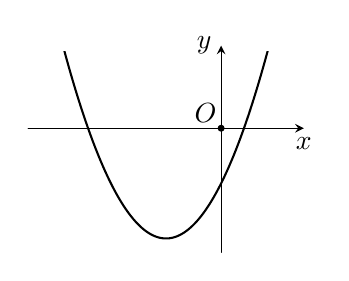
\begin{tikzpicture}[>=stealth,scale=0.7,line join=round, line cap=round]
			\def\xt{-3.5} \def\xp{1.5} \def\yd{-2.25} \def\yt{1.5}
			\draw[->] (\xt,0)--(\xp,0) node [below]{$x$};
			\draw[->] (0,\yd)--(0,\yt) node [left]{$y$};
			\draw[fill=black](0,0) circle (1.5pt) +(135:0.4)node{$O$};
			\clip (\xt+0.1,\yd+0.1) rectangle (\xp-0.1,\yt-0.1);
			
			\draw[smooth,samples=300,line width=0.75,domain=-3.5:1.5] plot(\x,{(\x)^(2)+2*(\x)-1});
		\end{tikzpicture}
	}
	\loigiai{
		\begin{itemize}
			\item Bề lõm của parabol hướng lên nên $a>0$.
			\item Parabol cắt trục tung tại điểm có tung độ âm nên $c<0$.
			\item Đỉnh của parabol có hoành độ âm nên $-\dfrac{b}{2a}<0 \Rightarrow b>0$.
		\end{itemize}	
	}
\end{ex}
%\begin{ex}%[0D2K3-3]
%	\immini{	Cho hàm số $y=ax^2+bx+c$ có đồ thị như hình bên. Khẳng định nào sau đây đúng?	
%		\choice
%		{$a>0,b<0,c>0$}
%		{\True $a>0,b>0,c<0$}
%		{$a>0,b<0,c<0$}
%		{$a>0,b>0,c>0$}
%	}{
%		\begin{tikzpicture}[scale=0.6,line join=round, line cap=round,>=stealth,transform shape]
%			\def \xmin{-3.1}
%			\def \xmax{3.1}
%			\def \ymin{-2.5}
%			\def \ymax{4.1}
%			\draw[->] (\xmin,0) -- (\xmax,0);
%			\draw[->,color=black] (0,\ymin) -- (0,\ymax);
%			\draw[color=black](\xmax-0.3,.2)node[right] {$x$};
%			\draw[color=black] (.1,\ymax) node[right] {\normalsize $y$};
%			\tkzDefPoints{0/0/O}
%			\tkzDrawPoints[fill=black](O)
%			\tkzLabelPoints[below left](O)
%			\begin{scope}
%				\clip(\xmin ,\ymin) rectangle (\xmax-.3,\ymax-.3);
%				%Vẽ đồ thị
%				\draw[color=black,smooth,samples=100,domain=-3.3:4.3] 
%				plot(\x,{(\x)^2+1*(\x)-2});
%			\end{scope}
%		\end{tikzpicture}
%	}
%	\loigiai{
%		Đồ thị hàm số hướng bề lõm lên trên nên hệ số $a>0$.\\
%		Đồ thị hàm số cắt trục tung tại điểm có tung độ âm, nên suy ra $c<0$.\\
%		Trục đối xứng của parabol thuộc bên trái trục tung, nên $-\dfrac{b}{2a}<0 \Leftrightarrow b>0$.}
%\end{ex}
\begin{ex}%[0D2B3-3]
	\immini
	{Cho hàm số $y=ax^2+bx+c$ có đồ thị như hình bên. Khẳng định nào sau đây đúng?	
		\choice
		{$a>0,b<0,c<0$}
		{$a<0,b<0,c>0$}
		{\True $a>0,b<0,c>0$}
		{$a>0,b>0,c>0$}}
	{\begin{tikzpicture}[scale=0.8, font=\footnotesize,line join=round, line cap=round, >=stealth]
			\def\xt{-1} \def\xp{3.5} \def\yt{3.5} \def\yd{-.7}
			\def\hs{(\x)^2-2*(\x)+1.5}
			\draw[->] (\xt,0)--(\xp,0) node [below]{$x$};
			\draw[->] (0,\yd)--(0,\yt) node [left]{$y$};
			\node at (0,0) [below left]{$O$};
			\clip (\xt-0.1,\yd+0.1) rectangle (\xp-0.1,\yt-0.1);
			\draw[smooth,samples=200,domain=-1:3] plot(\x,{\hs});
	\end{tikzpicture}}
	\loigiai{
		Dựa vào đồ thị $y=ax^2+bx+c$ ta có
		\begin{itemize}
			\item Đồ thị có bề lõm hướng lên trên nên $a>0$.
			\item Đồ thị cắt trục tung tại điểm có tung độ dương nên $c>0$.
			\item Trục đối xứng của đồ thị nằm bên phải $Oy$ nên $-\dfrac{b}{2a}>0$. Mà $a>0$ nên $b<0$.
	\end{itemize}}
\end{ex}
\begin{ex}%[0D2B3-3]
	\immini{
		Cho parabol $(P) \colon y=ax^2+bx+c$ có đồ thị như hình vẽ dưới đây. Hãy tìm khẳng định đúng
		\choice
		{$a>0;b>0;c>0$}
		{$a>0;b \geq 0;c<0$}
		{\True $a<0;b>0;c<0$}
		{$a<0;b \leq 0;c<0$}
	}{
		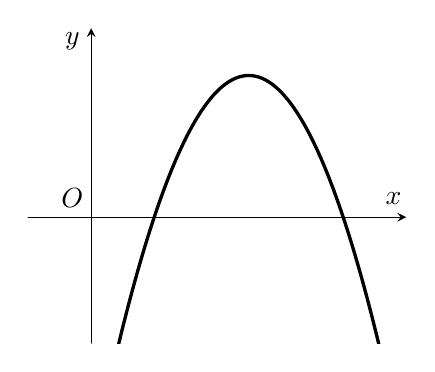
\begin{tikzpicture}[scale=0.8,line cap=round,line join=round,>=stealth,x=1cm,y=1cm]
			\draw[->,color=black] (-1,0) -- (5,0);
			\draw[->,color=black] (0,-2) -- (0,3);
			\clip(-1,-2) rectangle (5,3);
			\draw[line width=1.2pt,color=black,smooth,samples=100,domain=-0.5:4.8] plot(\x,{-1*(\x)^(2)+5*(\x)-4});
			\begin{normalsize}
				\draw[color=black] (-0.3,0.3) node {$O$};
				\draw[color=black] (4.8,0.3) node {$x$};
				\draw[color=black] (-0.3,2.8) node {$y$};
			\end{normalsize}
		\end{tikzpicture}
	}
	\loigiai{
		\begin{itemize}
			\item Đồ thị hướng bề lõm xuống dưới $\Rightarrow a<0$.
			\item Đồ thị có đỉnh có hoành độ dương $\Rightarrow -\dfrac{b}{2a}>0\overset{a<0} \Leftrightarrow b>0$.
		\end{itemize}
		Suy ra chọn \lq\lq $a<0;b>0;c<0$\rq\rq .
	}
\end{ex}
%\begin{ex}%[0D2B3-3]
%	\immini{
%		Cho parabol $(P)$ có phương trình $y=ax^2+bx+c\left(a \ne 0\right)$. $(P)$ có đồ thị như hình vẽ. Biết đồ thị của $(P)$ cắt trục $Ox$ tại các điểm có hoành độ lần lượt là $-2;2$. Tập nghiệm của bất phương trình $y<0$ là
%		\choice
%		{$S=(-\infty;-2] \cup [2;+\infty)$}
%		{\True $S=(-2;2)$}
%		{$S=[-2;2]$}
%		{$S=(-\infty;-2) \cup (2;+\infty)$}
%	}
%	{
%		\begin{tikzpicture}[scale=0.5, line width=1, >=stealth]
%			\draw[->](-3,0)--(3,0)node[above]{$x$};
%			\draw[->](0,-4.5)--(0,2)node[left]{$y$};
%			\draw[smooth,samples=100,domain=-2.3:2.3]plot(\x,{(\x)^2-4});
%			\node[above left] at (0,0) {$O$};
%			\draw[fill=black](2,0) circle(1pt) node[below  right] {\small$2$};
%			\draw[fill=black](-2,0) circle(1pt) node[below  left] {\small$-2$};
%		\end{tikzpicture}
%	}
%	\loigiai{
%		Ta thấy $y<0 \Leftrightarrow x \in (-2;2)$, do đó tập nghiệm của bất phương trình $y<0$ là $S=(-2;2)$.}
%\end{ex}
% \begin{ex}%[0D2K3-3]
% 	Cho hàm số $f(x)=ax^2+bx+c\left(a,b,c \ne 0\right)$ có đồ thị như hình vẽ bên. Biết rằng $f(c)=c$. Tính giá trị của $b$.
% 	\begin{center}
% 		\begin{tikzpicture}[=>stealth]
% 			\draw[->] (-1,0)--(3,0) node[below]{$x$};
% 			\draw[->] (0,-1)--(0,3) node[left]{$y$};
% 			\draw[samples=300] plot [domain=0.1:1.9](\x,{2*(\x)^2-4*(\x)+2});
% 			\coordinate[label=below left:$O$](O) at (0,0); % Vị trí đặt nhãn điểm là dưới trái điểm A
% 			\coordinate(I) at (1,0);
% 			\fill (O)circle(1.5pt) (I)circle(1.5pt);
% 		\end{tikzpicture}
% 	\end{center}
% 	\choice
% 	{\True $b=-4$}
% 	{$b=-2$}
% 	{$b=-\dfrac{5}{2}$}
% 	{$b=-6$}
% 	\loigiai{
% 		Ta có $f(c)=c \Rightarrow ac^2+bc+c=c \Leftrightarrow c(ac+b)=0 \Leftrightarrow ac=-b$ (vì $c \ne 0$ ).\\
% 		Dựa vào đồ thị ta thấy phương trình $f(x)=0$ có nghiệm kép do đó $\Delta =b^2-4ac=0$.\\
% 		Mà $ac=-b \Rightarrow b^2+4b=0 \Leftrightarrow \hoac{&b=0 \\& b=-4}$. Vì $b \ne 0$ nên $b=-4$.}
% \end{ex}
%\begin{ex}%[0D2K3-3]
%	\immini{
%		Cho hàm số $y=(x-1)(x+2)$ có đồ thị như hình bên. Xác định đồ thị của hàm số $y=|(x-1)(x+2)|$?
%	}{
%		\begin{tikzpicture}[scale=0.6,line join=round, line cap=round,>=stealth,transform shape]
%			\def \xmin{-3.1}
%			\def \xmax{3.1}
%			\def \ymin{-2.5}
%			\def \ymax{4.1}
%			\draw[->] (\xmin,0) -- (\xmax,0);
%			\draw[->,color=black] (0,\ymin) -- (0,\ymax);
%			\draw[color=black](\xmax-0.3,.2)node[right] {$x$};
%			\draw[color=black] (.1,\ymax) node[right] {\normalsize $y$};
%			\tkzDefPoints{0/0/O}
%			\tkzDrawPoints[fill=black](O)
%			\tkzLabelPoints[below left](O)
%			\begin{scope}
%				\clip(\xmin ,\ymin) rectangle (\xmax-.3,\ymax-.3);
%				%Vẽ đồ thị
%				\draw[color=black,smooth,samples=100,domain=-3.3:4.3] 
%				plot(\x,{(\x)^2+1*(\x)-2});
%			\end{scope}
%		\end{tikzpicture}
%	}
%	\choice
%	{\True \begin{tikzpicture}[scale=0.7,line join=round, line cap=round,>=stealth,transform shape]
%			\def \xmin{-3.1}
%			\def \xmax{3.1}
%			\def \ymin{-2.5}
%			\def \ymax{4.1}
%			\draw[->] (\xmin,0) -- (\xmax,0);
%			\draw[->,color=black] (0,\ymin) -- (0,\ymax);
%			\draw[color=black](\xmax-0.3,.2)node[right] {$x$};
%			\draw[color=black] (.1,\ymax) node[right] {\normalsize $y$};
%			\tkzDefPoints{0/0/O}
%			\tkzDrawPoints[fill=black](O)
%			\tkzLabelPoints[below left](O)
%			\begin{scope}
%				\clip(\xmin ,\ymin) rectangle (\xmax-.3,\ymax-.3);
%				%Vẽ đồ thị
%				\draw[color=black,smooth,samples=100,domain=-3.3:4.3] 
%				plot(\x,{abs((\x)^2+1*(\x)-2)});
%			\end{scope}
%	\end{tikzpicture} }
%	{\begin{tikzpicture}[scale=0.6,line join=round, line cap=round,>=stealth,transform shape]
%			\def \xmin{-3.1}
%			\def \xmax{3.1}
%			\def \ymin{-2.5}
%			\def \ymax{4.1}
%			\draw[->] (\xmin,0) -- (\xmax,0);
%			\draw[->,color=black] (0,\ymin) -- (0,\ymax);
%			\draw[color=black](\xmax-0.3,.2)node[right] {$x$};
%			\draw[color=black] (.1,\ymax) node[right] {\normalsize $y$};
%			\tkzDefPoints{0/0/O}
%			\tkzDrawPoints[fill=black](O)
%			\tkzLabelPoints[below left](O)
%			\begin{scope}
%				\clip(\xmin ,\ymin) rectangle (\xmax-.3,\ymax-.3);
%				%Vẽ đồ thị
%				\draw[color=black,smooth,samples=100,domain=-3.3:1] 
%				plot(\x,{-1*(\x)^2-1*(\x)+2});
%			\end{scope}
%			\begin{scope}
%				\clip(\xmin ,\ymin) rectangle (\xmax-.3,\ymax-.3);
%				\draw[color=black,smooth,samples=100,domain=1:4.3] 
%				plot(\x,{(\x)^2+1*(\x)-2});
%			\end{scope}
%	\end{tikzpicture} }
%	{\begin{tikzpicture}[scale=0.6,line join=round, line cap=round,>=stealth,transform shape]
%			\def \xmin{-3.1}
%			\def \xmax{3.1}
%			\def \ymin{-3.5}
%			\def \ymax{4.1}
%			\draw[->] (\xmin,0) -- (\xmax,0);
%			\draw[->,color=black] (0,\ymin) -- (0,\ymax);
%			\draw[color=black](\xmax-0.3,.2)node[right] {$x$};
%			\draw[color=black] (.1,\ymax) node[right] {\normalsize $y$};
%			\tkzDefPoints{0/0/O}
%			\tkzDrawPoints[fill=black](O)
%			\tkzLabelPoints[below left](O)
%			\begin{scope}
%				\clip(\xmin ,\ymin) rectangle (\xmax-.3,\ymax-.3);
%				%Vẽ đồ thị
%				\draw[color=black,smooth,samples=100,domain=-2:4] 
%				plot(\x,{(\x)^2+1*(\x)-2});
%			\end{scope}
%			\begin{scope}
%				\clip(\xmin ,\ymin) rectangle (\xmax-.3,\ymax-.3);
%				\draw[color=black,smooth,samples=100,domain=-3:-2] 
%				plot(\x,{-1*(\x)^2-1*(\x)+2});
%			\end{scope}
%	\end{tikzpicture}}
%	{\begin{tikzpicture}[scale=0.6,line join=round, line cap=round,>=stealth,transform shape]
%			\def \xmin{-3.1}
%			\def \xmax{3.5}
%			\def \ymin{-2.5}
%			\def \ymax{4.1}
%			\draw[->] (\xmin,0) -- (\xmax,0);
%			\draw[->,color=black] (0,\ymin) -- (0,\ymax);
%			\draw[color=black](\xmax-0.3,.2)node[right] {$x$};
%			\draw[color=black] (.1,\ymax) node[right] {\normalsize $y$};
%			\tkzDefPoints{0/0/O}
%			\tkzDrawPoints[fill=black](O)
%			\tkzLabelPoints[below left](O)
%			\begin{scope}
%				\clip(\xmin ,\ymin) rectangle (\xmax-.3,\ymax-.3);
%				%Vẽ đồ thị
%				\draw[color=black,smooth,samples=300,domain=-3.3:6.3] 
%				plot(\x,{abs((\x)^2-1*(\x)-2});
%			\end{scope}
%	\end{tikzpicture} }
%	\loigiai{
%		Từ đồ thị $(P)$ của hàm số $y=(x-1)(x+2)$ ta suy ra đồ thị $(P')$ của hàm số $y=|(x-1)(x+2)|$ như sau
%		\begin{itemize}
%			\item Giữ nguyên phần đồ thị $(P)$ nằm phía trên trục $Ox$.
%			\item Lấy đối xứng phần đồ thị $(P)$ nằm phía dưới trục $Ox$ lên phía trên trục $Ox$.
%		\end{itemize}
%		Hợp các phần đồ thị trên ta được đồ thị $(P')$.}
%\end{ex}
%\begin{ex}%[0D2G3-3]
%	\immini{Cho đồ thị hàm số $y=f(x)=ax^2+bx+c,\left(a \ne 0\right)$ có đồ thị như hình vẽ. Gọi $S$ là tập hợp tất cả các giá trị nguyên của $m$ để phương trình $ax^2+b|x|+c=m$ có đúng hai nghiệm $x_1;x_2$ sao cho $-3<x_1<x_2<3$. Tính tổng các phần tử của $S$.
%		\choice
%		{$2$}
%		{$-7$}
%		{\True $-3$}
%		{$3$}}
%	{\begin{tikzpicture}[scale=0.7,>=stealth] 
%			\draw[->](-1.5,0)--(3.8,0)node[above]{$x$};
%			\draw[->](0,-4.5)--(0,1.5)node[right]{$y$};
%			\draw[smooth,samples=100,domain=-1.3:3.3]plot(\x,{\x*\x -2*\x-3});
%			\fill (0,0)node[above left]{O}circle(1.2pt)	(3,0)node[above left]{$3$}circle(1.2pt) (0,-3)node[left]{$-3$}circle(1.2pt) (0,-4)node[left]{$-4$}circle(1.2pt);
%			\draw[dashed](1,0)--(1,-4)--(0,-4);
%	\end{tikzpicture}}
%	\loigiai{
%		Nhận xét phương trình $ax^2+b|x|+c=m$ nếu có nghiệm $x_0$ thì $-x_0$ cũng là nghiệm.\\
%		Để $ax^2+b|x|+c=m$ có đúng hai nghiệm $x_1;x_2$ sao cho $-3<x_1<x_2<3$. \\
%		Thì phương trình $ax^2+b|x|+c=m$ trên miền $[0;3]$ có đúng $1$ nghiệm $0<x_2<3$. \\
%		Hay $ax^2+bx+c=m$ trên miền $[0;3]$ có đúng $1$ nghiệm $0<x_2<3$. \\
%		Dựa vào đồ thị ta có: $-3<m<0$ mà $m$ nguyên nên $m=-2$, $m=-1$. \\
%		Vậy tổng các giá trị bằng $-3$.}
%\end{ex}

%\begin{ex}%[0D2G3-3]
%	\immini{Cho hai hàm số $y=a_1 x^2+b_1 x +c_1$ và $y=a_2 x^2+b_2 x + c_2$ với $a_1$, $a_2$, $b_1$, $b_2$, $c_1$, $c_2$ là các số thực, lần lượt có đồ thị là $(C_1)$ và $(C_2)$ như hình bên. Mệnh đề nào dưới đây đúng?
%		\choice
%		{$a_1>a_2, b_1<b_2, c_1>c_2$}
%		{$a_1>a_2, b_1>b_2, c_1>c_2$}
%		{$a_1<a_2, b_1<b_2, c_1<c_2$}
%		{\True $a_1<a_2, b_1>b_2, c_1<c_2$}
%	}
%	{
%		\begin{tikzpicture}[>=stealth, x=1cm, y=1cm, scale=0.45]
%			\begin{scriptsize}
%				\def\xmin{-2.5} \def\xmax{6} \def\ymin{-3} \def\ymax{4};
%				\draw [->] (\xmin-.2, 0)--(\xmax+.2, 0) node[below]{$x$};
%				\draw [->] (0, \ymin-.2)--(0, \ymax+.2) node[right]{$y$};
%				\draw [fill=black] circle (1pt) node [below left]{$O$};
%				\draw (2,-2.5) node [right]{$(C_1)$} (6,3) node [left]{$(C_2)$};
%				\draw[smooth,domain=-2:2] plot(\x,{(-1)*(\x)^(2)+1});
%				\draw[smooth,domain=-0.5:6.5] plot(\x,{(1/3)*(\x)^(2)-2*(\x)+3});
%			\end{scriptsize}
%		\end{tikzpicture}
%	}	
%	\loigiai{Từ hai đồ thị ta có $a_1<0,b_1=0,a_2>0,b_2<0$ và $c_1<c_2$. 
%		Do đó ta chọn kết quả $a_1<a_2, b_1>b_2, c_1<c_2$.}
%\end{ex}
\begin{ex}%[0D2B3-4]
	Tìm số giao điểm của parabol $(P) \colon y=x^2-3x+5$ với trục $Ox$.
	\choice
	{$3$}
	{\True $0$}
	{$1$}
	{$2$}
	\loigiai{
		Xét phương trình hoành độ giao điểm của $(P)$ với $Ox$ là $x^2-3x+5=0$ có $\Delta =9-20=-11<0$ nên phương trình vô nghiệm.\\ 
		Vậy không có giao điểm của $(P)$ với $Ox$.
	}
\end{ex}
\begin{ex}%[0D2B3-4]
	Giao điểm của parabol $y=x^2-3x+2$ với đường thẳng $y=x-1$ là
	\choice
	{$(2;1), (3;2)$}
	{\True $(1;0), (3;2)$}
	{$(0;-1), (-2;-3)$}
	{$(-1;2), (2;1)$}
	\loigiai{
		Phương trình hoành độ giao điểm: $x^2-3x+2=x-1 \Leftrightarrow \hoac{&x=1 \Rightarrow y=0 \\& x=3 \Rightarrow y=2.}$}
\end{ex}
\begin{ex}%[0D2B3-4]
	Tọa độ giao điểm của $(P)\colon y=x^2-4x$ với đường thẳng $d\colon y=-x-2$ là
	\choice
	{$M(0;-2)$; $N(2;-4)$}
	{$M(-1;-1)$; $N(-2;0)$}
	{$M(-3;1)$; $N(3;-5)$}
	{\True $M(1;-3)$; $N(2;-4)$}
	\loigiai{
		Hoành độ giao điểm của $(P)$ và $(d)$ là nghiệm của phương trình
		\[x^2-4x=-x-2 \Leftrightarrow x^2-3x+2=0 \Leftrightarrow \hoac{&x=1 \\& x=2.}\]
		Vậy tọa độ giao điểm là $M(1;-3)$; $N(2;-4)$.
	}
\end{ex}
\begin{ex}%[0D2B3-4]
	Parabol nào sau đây cắt trục hoành tại hai điểm phân biệt?
	\choice
	{$y=-x^2+2x-1$}
	{$y=x^2-2x+3$}
	{$y=-x^2-1$}
	{\True $y=2x^2-5x+2$}
	\loigiai{
		Ta có $2x^2-5x+2=0 \Leftrightarrow \hoac{& x=2 \\& x=\dfrac{1}{2}}$ nên parabol $y=2x^2-5x+2$ cắt trục hoành tại hai điểm phân biệt.}
\end{ex}
\begin{ex}%[0D2Y3-4]
	Tổng tung độ hai giao điểm của parapol $(P) \colon y=x^2-5x+6$ và đường thẳng $(d) \colon y=2x-2$ bằng
	\choice
	{$7+2\sqrt{17}$}
	{$12$}
	{$2\sqrt{17}-4$}
	{\True $10$}
	\loigiai{
		Phương trình hoành độ giao điểm của parapol $(P) \colon y=x^2-5x+6$ và đường thẳng $(d) \colon y=2x-2$:\\
		$$x^2-5x+6=2x-2 \Leftrightarrow x^2-7x+8=0 \Leftrightarrow \hoac{&x=\dfrac{7-\sqrt{17}}{2} \\& x=\dfrac{7+\sqrt{17}}{2}.}$$\\
		$x=\dfrac{7-\sqrt{17}}{2} \Rightarrow y=2x-2=5-\sqrt{17}$ \\
		$x=\dfrac{7+\sqrt{17}}{2} \Rightarrow y=2x-2=5+\sqrt{17}$ \\
		Tổng tung độ hai giao điểm bằng $10$.}
\end{ex}
\begin{ex}%[0D2G3-4]
	\immini
	{
		Cho hàm số $y=f(x)$ xác định trên $\mathbb{R}$ có đồ thị như hình vẽ. Phương trình $2f(x)-1=0$ có bao nhiêu nghiệm?
		\choice
		{$1$}
		{\True $3$}
		{$2$}
		{$4$}
	}
	{
		\begin{tikzpicture}[>=stealth,x=0.7cm,y=0.71cm]
			\draw[->] (-2,0)--(4,0) node[below]{\footnotesize $x$};
			\foreach \x in {2}
			\draw[shift={(\x,0)},color=black] (0pt,2pt) -- (0pt,-2pt) node[above] { $\x$};
			\draw[->] (0,-4)--(0,2.3) node[right]{\footnotesize $y$};
			\foreach \y in {1,-3}
			\draw[shift={(0,\y)},color=black] (2pt,0pt) -- (-2pt,0pt) node[left] {\normalsize $\y$};
			\draw (0,0) node[below right]{$O$};
			\draw[dashed] (2,0)--(2,-3)--(0,-3);
			\draw[smooth,domain=-1.1:3.1] plot(\x,{1*(\x)^3-3*(\x)^2+1});
			\fill (0,0) circle (1.0pt);
		\end{tikzpicture}
	}
	\loigiai{
		Ta có $2f(x)-1=0 \Leftrightarrow f(x)=\dfrac{1}{2}$.\\
		Dựa vào đồ thị ta thấy đường thẳng $y=\dfrac{1}{2}$ cắt đồ thị hàm số $y=f(x)$ tại $3$ điểm phân biệt.\\
		Vậy phương trình $2f(x)-1=0$ có $3$ nghiệm phân biệt.}
\end{ex}
\begin{ex}%[0D2B3-4]
	Đồ thị hàm số $y=x^2+5$ và $y=-mx+1$ cắt nhau tại một điểm thì $m$ bằng
	\choice
	{\True $m=4$ hoặc $m=-4$}
	{$m=0$ hoặc $m=4$}
	{$m=0$ hoặc $m=-4$}
	{$m=0$ hoặc $m=-4$ hoặc $m=4$}
	\loigiai{
		Ta có phương trình hoành độ giao điểm $x^2+5=-mx+1\Leftrightarrow x^2+mx+4=0$. Phương trình có một nghiệm khi và chỉ khi $\Delta'=0\Leftrightarrow m^2-16=0\Leftrightarrow m=\pm 4$.
	}
\end{ex}
\begin{ex}%[0D2B3-4]
	Đồ thị hàm số $y=x^2+5$ và $y=-mx+1$ cắt nhau tại hai điểm phân biệt khi 
	\choice
	{$m>4$}
	{$m<-4$}
	{$-4<m<4$}
	{\True $m>4$ hoặc $m<-4$}
	\loigiai{
		Ta có phương trình hoành độ giao điểm $x^2+5=-mx+1\Leftrightarrow x^2+mx+4$.\\
		Phương trình có hai nghiệm phân biệt khi và chỉ khi $\Delta'>0\Leftrightarrow m^2-16>0\Leftrightarrow \hoac{& m>4 \\ & m<-4.}$
	}
\end{ex}

\begin{ex}%[0D2B3-4]
	Có bao nhiêu giá trị nguyên của $m$ để đường thẳng $y=mx-3$ không có điểm chung với Parabol $y=x^2+1$?
	\choice
	{$6$}
	{$9$}
	{\True $7$}
	{$8$}
	\loigiai{
		Phương trình hoành độ giao điểm:
		$x^2+1=mx-3 \Leftrightarrow x^2-mx+4=0$. \hfill$(1)$ \\
		Ta có $\Delta = (-m)^2 - 4\cdot 1\cdot 4 = m^2 -16$.\\
		Để đường thẳng và Parabol không có điểm chung thì phương trình $(1)$ vô nghiệm\\
		$\Leftrightarrow \Delta = m^2-16<0 \Leftrightarrow -4<m<4 \Rightarrow m \in \{-3;-2;-1;0;1;2;3\}$.}
\end{ex}
%\begin{ex}%[0D2K3-4]
%	Tìm tất cả các giá trị của tham số $m$ để đồ thị hàm số $y=x^2+2mx+m^2-3m+1$ cắt trục hoành tại hai điểm phân biệt.
%	\choice
%	{$m<\dfrac{1}{3}$}
%	{$m=-1$}
%	{$m<0$}
%	{\True $m>\dfrac{1}{3}$}
%	\loigiai{
%		Đồ thị hàm số $y=x^2+2mx+m^2-3m+1$ cắt trục hoành tại hai điểm phân biệt\\
%		$\Leftrightarrow x^2+2mx+m^2-3m+1=0$ có hai nghiệm phân biệt\\
%		$\Leftrightarrow {\Delta}'=3m-1>0 \Leftrightarrow m>\dfrac{1}{3}$.}
%\end{ex}
\begin{ex}%[0D2K3-4]
	Cho hàm số $y=-x^2-2x+5$ có đồ thị bên\\
	\immini{
		Tất cả giá trị của $m$ để đường thẳng $y=m$ cắt parabol $(P)$ tại hai điểm phân biệt trong đó có đúng $1$ điểm có hoành độ lớn hơn $1$.
		\choice
		{$m>2$}
		{$m<1$}
		{\True $m<2$}
		{$m>1$}
	}{\begin{tikzpicture}[xscale=0.5,yscale=0.3, font=\footnotesize, line join=round, line cap=round, >=stealth]
			\clip(-4,-1.3) rectangle (2,7);
			\draw [samples=50,rotate around={-180:(-1,6)},xshift=-1cm,yshift=6cm,line width=0.4pt,domain=-5:5)] plot (\x,{(\x)^2/2/0.5});
			\draw [line width=0.4pt,dash pattern=on 2pt off 2pt] (-1,-3.367) -- (-1,8.97);
			\draw [line width=0.4pt,dash pattern=on 2pt off 2pt] (0,2)-- (1,2);
			\draw [line width=0.4pt,dash pattern=on 2pt off 2pt] (1,2)-- (1,0);
			\draw [line width=0.4pt,dash pattern=on 2pt off 2pt] (-1,6)-- (0,6);
			\draw [->,line width=0.4pt] (-5,0) -- (2,0);
			\draw [->,line width=0.4pt] (0,-1) -- (0,7);
			\begin{scriptsize}
				\draw (-2,-0.04) node[anchor=north west] {$-1$};
				\draw (0.55,-0.04) node[anchor=north west] {$1$};
				\draw (-0.7,2.5) node[anchor=north west] {$2$};
				\draw (-0.7,7.2) node[anchor=north west] {$y$};
				\draw (1.5,0.1) node[anchor=north west] {$x$};
				\draw (0.01,6.55) node[anchor=north west] {$6$};
				\draw (-0.8,-0.04) node[anchor=north west] {$O$};
				\draw [fill=black] (0,2) circle (1pt);
				\draw [fill=black] (1,2) circle (1pt);
				\draw [fill=black] (1,0) circle (1pt);
				\draw [fill=black] (-1,6) circle (1pt);
				\draw [fill=black] (0,6) circle (1pt);
			\end{scriptsize}
	\end{tikzpicture}}
	\loigiai{
		Ta có: $x>1$ thì $-x^2<-1; -2x<-2$, suy ra: $y = -x^2-2x+5<2$.
		Vậy $m<2$.\\
		Cách 2: Nhìn trên đồ thị ta thấy với $x>1$ thì $y<2$ hay $m<2$.
	}
\end{ex}
%\begin{ex}%[0D2K3-4]
%	Cho parabol $(P) \colon y=\dfrac{x^2}{2}$ và đường thẳng $d \colon y=(m-1)x+\dfrac{m+3}{2}$. Tìm tham số $m$ để hai đồ thị hàm số trên cắt nhau tại hai điểm phân biệt $A$, $B$ sao cho $x_A^2+x_B^2 \geq 10$.
%	\choice
%	{$m<\dfrac{3}{2}$}
%	{\True $\hoac{&m \geq \dfrac{3}{2} \\& m \leq 0}$}
%	{$m>0$}
%	{$0 \leq m \leq \dfrac{3}{2}$}
%	\loigiai{
%		Phương trình hoành độ giao điểm của $(P)$ và $d$:\\
%		$\dfrac{x^2}{2}=(m-1)x+\dfrac{m+3}{2} \Leftrightarrow x^2-2(m-1)x-(m+3)=0$ (*).\\
%		Để $(P)$ và $d$ cắt nhau tại hai điểm phân biệt thì phương trình (*) phải có hai nghiệm phân biệt.\\
%		$\Leftrightarrow (m-1)^2+(m+3)>0 \Leftrightarrow m^2-m+4>0$ luôn đúng $\forall m \in \mathbb{R}$.\\
%		Khi đó $x_A,x_B$ là hai nghiệm của (*) thoả mãn $\heva{&x_A+x_B=2(m-1) \\& x_A \cdot x_B=-(m+3).}$\\
%		Mà $x_A^2+x_B^2 \geq 10 \Leftrightarrow (x_A+x_B)^2-2x_A \cdot x_B \geq 10 \Leftrightarrow 4(m-1)^2+2(m+3) \geq 10 \Leftrightarrow 2m^2-3m \geq 0\\ \Leftrightarrow \hoac{&m \geq \dfrac{3}{2} \\& m \leq 0.}$\\
%		Kết hợp điều kiện, ta có $\hoac{&m \geq \dfrac{3}{2} \\& m \leq 0.}$}
%\end{ex}
\begin{ex}%[0D2K3-4]
	Cho hàm số bậc hai $f(x)=ax^2+bx+c$ có bảng biến thiên như hình vẽ. 
	\begin{center}
		\begin{tikzpicture}
			\tkzTabInit[nocadre=false, lgt=1, espcl=3]{$x$ /1,$y$ /2}{$-\infty$,$0$,$1$,$+\infty$}
			\tkzTabVar{+/$+\infty$,R,  -/$-3$,+/$+\infty$}
			\tkzTabVal{1}{3}{0.5}{}{$-1$}
		\end{tikzpicture}
	\end{center}
	Có bao nhiêu giá trị nguyên của tham số $m$ thuộc đoạn $[-2018;2018]$ để phương trình $f(x)-m-4=0$ có một nghiệm dương duy nhất.
	\choice
	{$2026$}
	{$2020$}
	{$2025$}
	{\True $2024$}
	\loigiai{
		\\
		Phương trình $f(x)-m-4=0 \Leftrightarrow f(x)=m+4$ có một nghiệm dương duy nhất khi và chỉ khi đồ thị hàm số $y=f(x)$ cắt đường thẳng $y=m+4$ cắt nhau tại duy nhất một điểm có hoành độ dương $$\Leftrightarrow \hoac{&m+4=-3 \\& m+4 \geq -1}\Leftrightarrow \hoac{&m=-7 \\& m \geq -5.}$$
		Do $m$ thuộc đoạn $[-2018;2018]$ và nguyên nên có $2024$ giá trị thỏa mãn.}
\end{ex}
%\begin{ex}%[0D2K3-4]
%	\immini{
%		Hàm số $y=x^2+4x-1$ có bảng biến thiên như hình vẽ. Có bao nhiêu giá trị nguyên của $m$ để phương trình $|-x^2-4x+1|=m$ có $4$ nghiệm phân biệt?	
%		\choice
%		{$3$}
%		{Vô số}
%		{\True $4$}
%		{$0$}
%	}{
%		\begin{tikzpicture}
%			\tkzTabInit[nocadre=false,lgt=0.7,espcl=2.5]
%			{$x$ /0.6,$y$ /2}
%			{$-\infty$,$-2$,$+\infty$}
%			\tkzTabVar{ +/$+\infty$,-/$-5$,+/$+\infty$}
%		\end{tikzpicture}
%	}
%	\loigiai{
%		Ta có phương trình $|-x^2-4x+1|=m$ có $4$ nghiệm phân biệt $\Leftrightarrow \heva{&m>0 \\& \hoac{&x^2+4x-1=m \\& x^2+4x-1=-m}}$ có 4 nghiệm phân biệt $\Leftrightarrow \heva{&m>0 \\& m>-5 \\& -m>-5}\Leftrightarrow 0<m<5$. \\
%		Do $m \in \mathbb{Z}$ nên $m \in \{1;2;3;4\}$.\\
%		Vậy có $4$ giá trị nguyên của tham số $m$.}
%\end{ex}
%\begin{ex}%[0D2K3-4]
%	\immini{
%		Cho hàm số $y=f(x)=ax^2+bx+c$ có đồ thị như hình vẽ. Gọi $S$ là tập hợp các giá trị nguyên của $m$ để phương trình $f(|x|)-1=m$ có $4$ nghiệm phân biệt. Số phần tử của $S$ là
%		\choice
%		{$1$}
%		{$2$}
%		{\True $3$}
%		{$4$}
%	}{
%		\begin{tikzpicture}[scale=0.7, font=\footnotesize, line join=round, line cap=round,>=stealth]
%			\draw[->] (-1.1,0)--(0,0) node[below left]{$O$}--(4,0) node[below]{$x$};
%			\draw[->] (0,-1.5) --(0,4) node[right]{$y$};
%			\foreach \x in {-1,1,2,3}{
%				\draw (\x,0) node[below left]{$\x$} circle (1pt);
%				\draw (0,\x) node[left]{$\x$} circle (1pt);
%			}
%			\draw [ domain=-0.25:4.25, samples=100] %
%			plot (\x, {(\x)^2-4*(\x)+3});
%			\draw [dashed] (2,0)--(2,-1)--(0,-1);
%			\fill (0,0) circle (1.0pt);
%		\end{tikzpicture}
%	}
%	\loigiai{		
%		Ta có đồ thị của hàm số $y=f(|x|)$
%		\begin{center}
%			\begin{tikzpicture}[>=stealth]
%				\draw[->,line width = 1pt] (-3,0)--(0,0) node[below left]{$O$}--(4,0) node[below]{$x$};
%				\draw[->,line width = 1pt] (0,-3) --(0,4) node[right]{$y$};
%				\foreach \x in {-2,-1,1,2,3}{
%					\draw (\x,0) node[below left]{$\x$} circle (1pt);
%					\draw (0,\x) node[left]{$\x$} circle (1pt);
%				}
%				\draw [ domain=-4.25:0, samples=100] %
%				plot (\x, {(\x)^2+4*(\x)+3});
%				\draw [ domain=0:4.25, samples=100] %
%				plot (\x, {(\x)^2-4*(\x)+3});
%				\draw [dashed] (2,0)--(2,-1)--(0,-1)--(-2,-1)--(-2,0);
%			\end{tikzpicture}
%		\end{center}
%		Phương trình $f(|x|)-1=m\Leftrightarrow f(|x|)=m+1$. Số nghiệm của phương trình bằng số giao điểm của đồ thì hàm số $y=f(|x|)$ và đường thẳng $y=m+1$. Từ đồ thị ta có phương trình có $4$ nghiệm khi và chỉ khi $-1<m+1<3\Leftrightarrow -1<m<2$. Vậy có $3$ giá trị $m\in\mathbb{Z}$.
%	}
%\end{ex}
%\begin{ex}%[0D2K3-4]
%	\immini{
%		Cho hàm số $y=f(x)=ax^2+bx+c$ có đồ thị $(C)$ như hình vẽ bên.\\
%		Có bao nhiêu giá trị nguyên của tham số $m$ để phương trình $f^2\left(|x|\right)+(m-2)f\left(|x|\right)+m-3=0$ có 6 nghiệm phân biệt ?
%		\choice
%		{$1$}
%		{$4$}
%		{\True $3$}
%		{$2$}
%	}{
%		\begin{tikzpicture}[scale = 0.85]
%			\draw[thick, ->] (-1,0) -- (0,0) node[above left]{$O$} -- (5,0) node[below]{$x$};
%			\draw[thick, ->] (0,-1.5) -- (0,5) node[left]{$ y $};
%			\draw[line width=1pt, color = blue] plot[domain=-0.25:4.25, samples=100] (\x,{(\x)^(2.0)-4.0*(\x)+3.0});
%			\draw [dashed] (2,0) circle (1pt) node[above]{$ 2 $} -- (2,-1) circle (2pt) -- (0,-1) circle (1pt) node[left]{$-1$};
%			\tkzDrawPoint[fill = black](0,0);
%			\draw (1,0) circle (1pt) node[below left]{$ 1 $};
%			\draw (3,0) circle (1pt) node[below right]{$ 3 $};
%			\draw (0,3) circle (1pt) node[left]{$ 3 $};
%		\end{tikzpicture}
%	}
%	\loigiai{
%		Đặt $t=f\left(|x|\right)$, phương trình trở thành $t^2+(m-2)t+m-3=0 \Leftrightarrow \hoac{&t=-1 \\& t=3-m.}$\\
%		Suy ra $\hoac{&f\left(|x|\right)=-1 \quad (1) \\& f\left(|x|\right)=3-m \quad (2).}$\\
%		Từ đồ thị của $y=f(x)$ ta suy ra đồ thị của $y=f\left(|x|\right)$:
%		\begin{center}
%			\begin{tikzpicture}[scale = 0.7]
%				\draw[thick, ->] (-5.5,0) -- (0,0) node[above left]{$O$} -- (5.5,0) node[below]{$x$};
%				\draw[thick, ->] (0,-2) -- (0,9) node[left]{$ y $};
%				\draw[line width=1pt, color = black] plot[domain=-5:5, samples=100] (\x,{abs((\x))^(2.0)-4.0*abs((\x))+3.0});
%				\draw [dashed] (2,0) circle (1pt) node[above]{$ 2 $} -- (2,-1) circle (2pt) -- (0,-1) circle (1pt) node[below left]{$-1$} -- (-2,-1) circle (2pt) -- (-2,0) circle (1pt) node[above]{$ -2 $};
%				\tkzDrawPoint[fill = black](0,0);
%				\draw (1,0) circle (1pt) node[below left]{$ 1 $};
%				\draw (3,0) circle (1pt) node[below right]{$ 3 $};
%				\draw (-1,0) circle (1pt) node[below right]{$ -1 $};
%				\draw (-3,0) circle (1pt) node[below left]{$ -3 $};
%				\draw (0,3) circle (1pt) node[left]{$ 3 $};
%			\end{tikzpicture}
%		\end{center}
%		Vì phương trình (1) cho 2 nghiệm là $-2$ và $2$ nên yêu cầu bài toán $\Leftrightarrow$ phương trình (2) có 4 nghiệm phân biệt $\Leftrightarrow$ $-1<3-m<3 \Leftrightarrow 0<m<4$.\\
%		Vậy có 3 giá trị nguyên $m$ là $1$; $2$; $3$.}
%\end{ex}
%\begin{ex}%[0D2B3-5]
%	Một vật chuyển động với vận tốc $v=5+2t-t^2$ (m/s). Trong $3$ giây đầu, vận tốc lớn nhất của vật là bao nhiêu?
%	\choice
%	{$1$ m/s}
%	{\True $6$ m/s}
%	{$5$ m/s}
%	{$4$ m/s}
%	\loigiai{
%		Ta có $v=5+2t-t^2=-(t-1)^2+6 \leq 6$. Dấu bằng xảy ra khi $t=1 \in (0;3]$.\\
%		Vậy trong $3$ giây đầu, vận tốc lớn nhất của vật là $6$ m/s.}
%\end{ex}
% \begin{ex}%[0D2K3-5]
% 	Vận tốc chuyển động của một vật được biểu thị bởi hàm số $v(t)=at^2+bt+c$, trong đó $t$ là thời gian tính theo giây và $a$, $b$, $c$ là các hằng số. Tại thời điểm $1$ giây, $2$ giây và $5$ giây vận tốc của vật lần lượt là $16$ (m/s), $21$ (m/s) và $24$ (m/s). Tại thời điểm nào vận tốc của vật lớn nhất?
% 	\choice
% 	{$5$ giây}
% 	{\True $4$ giây}
% 	{$6$ giây}
% 	{$3$ giây}
% 	\loigiai{
% 		Ta có $\heva{&v(1)=16\\&v(2)=21\\&v(5)=24}\Leftrightarrow \heva{&a+b+c=16\\&4a+2b+c=21\\&25a+5b+c=24}\Leftrightarrow \heva{&a=-1\\&b=8\\&c=9.}$\\
% 		Do đó $v(t)=-t^2+8t+9$.\\
% 		Vì $a=-1<0$ nên vận tốc của vật lớn nhất tại thời điểm $t=-\dfrac{b}{2a}=-\dfrac{8}{2(-1)}=4$ (giây).
% 	}
% \end{ex}
\begin{ex}%[0D2T3]
	Một vật chuyển động với vận tốc $v=40+18t-t^2$ (m/s). Trong $20$ giây đầu vận tốc lớn nhất của vật là bao nhiêu?
	\choice{\True $121$ m/s}
	{$212$ m/s}
	{$40$ m/s}
	{$4$ m/s}
	\loigiai{
		\immini{Đồ thị của hàm vận tốc $v$ có dạng Parabol  bề lõm hướng xuống dưới. Đỉnh của Parabol là $I(9;121)$. Do đó trong đoạn $[0;20]$, vận tốc lớn nhất của vật là $121$ m/s.
		}{
			\begin{tikzpicture}[line cap=round,line join=round,>=stealth,x=0.1cm,y=0.1cm, scale=0.4]
				\draw[->,color=black] (0,0.) -- (30,0.);
				\foreach \x in {9,20}
				\draw[shift={(\x,0)},color=black] (0pt,2pt) -- (0pt,-2pt) node[below] {\footnotesize $\x$};
				\draw[->,color=black] (0.,0) -- (0.,130);
				\foreach \y in {121}
				\draw[shift={(0,\y)},color=black] (2pt,0pt) -- (-2pt,0pt) node[left] {\footnotesize $\y$};
				\draw[color=black] (0pt,-10pt) node[left] {\footnotesize $O$};
				\clip(0,0) rectangle (30,130);
				\draw[line width=1.0pt,color=black,smooth,samples=100,domain=0:20] plot(\x,{40+18*\x-(\x)^2});
				\draw [dash pattern=on 2pt off 2pt] (9,0)--(9,121)--(0,121);
				\draw (28, 3)  node {$x$}; \draw (3,128)  node {$y$};
			\end{tikzpicture}
	}}
\end{ex}
\begin{ex}%[0D2T3-5]
	Một quả bóng chày được đánh lên ở độ cao $3$ feet ($1$ feet $ = 0,3048$ mét) so với mặt đất với vận tốc $100$ feet/giây và ở một góc $45^\circ$ so với mặt đất. Đường đi của quả bóng chày được cho bởi hàm số $f(x)=-0,0032x^2+x+2$ trong đó $f(x)$ là chiều cao của bóng chày (theo feet) và $x$ là khoảng cách theo chiều ngang của quả bóng tính từ vị trí ban đầu của quả bóng được đánh lên (theo feet). Tính chiều cao tối đa mà bóng chày đạt được?
	\choice
	{$78,125$ feet}
	{$79,125$ feet}
	{\True $80,125$ feet}
	{$81,125$ feet}
	\loigiai{
		Chiều cao tối đa $h$ của quả bóng là tung độ đỉnh của đồ thị hàm số $f(x)=-0,0032x^2+x+2$. \\
		Ta tính được $h=80,125$.
	}
\end{ex}

%\begin{ex}%[0D2T3-5]
%	Một quả bóng được ném qua một sân chơi từ độ cao $6$ feet ($1$ feet $ = 0,3048$ mét) so với mặt đất theo một góc $45^\circ$ so với phương ngang với vận tốc $20$ feet/giây. Dựa vào các nguyên lý về vật lý, người ta tính được đường đi của quả bóng được mô tả bởi hàm số $\displaystyle y=-\dfrac{32}{(20)^2}x^2+x+5$. Hãy tính độ xa theo chiều ngang của quả bóng kể từ vị trí người đứng ném đến vị trí bóng chạm đất (làm tròn đến chữ số thập phân thứ 2).
%	\choice
%	{$16,33$ feet}
%	{\True $15,23$ feet}
%	{$14,33$ feet}
%	{$17,23$ feet}
%	\loigiai{
%		\immini{
%			Bài toán được mô tả như hình vẽ.\\ Quả bóng chạm đất khi $y=0$.\\
%			Khi đó $x_1=\dfrac{25-5\sqrt{65}}{4}, x_2=\dfrac{25+5\sqrt{65}}{4}$.\\
%			Ở vị trí quả bóng được ném lên thì $y=6$,\\ suy ra vị trí ban đầu của quả bóng là $x_0=\dfrac{25-5\sqrt{17}}{4}$.\\
%			Vậy độ xa của quả bóng là:\\ $x_2-x_0 = \dfrac{5\sqrt{65}+5\sqrt{17}}{4} \approx 15,23$.
%		}
%		{
%			\begin{tikzpicture}[>=stealth, x=0.4cm, y=0.5cm, scale=0.7]
%				\begin{scriptsize}
%					\def\xmin{-5} \def\xmax{18} \def\ymin{-2} \def\ymax{9};
%					\draw [->] (\xmin-.2, 0)--(\xmax+.2, 0) node[below]{$x$};
%					\draw [->] (0, \ymin-.2)--(0, \ymax+.2) node[right]{$y$};
%					\draw node [below left]{$O$};
%					\draw (0,5) node [left]{$5$} (0,6) node [left]{$6$} (-3.3,0) node [above left]{$x_1$} (16.3,0) node [above right]{$x_2$} (1.1,0) node [below]{$x_0$} ;
%					\draw [fill=black] (1.1,6) circle (5pt);
%					\draw [dashed] (1.1,0)--(1.1,6)--(0,6);
%					\draw[smooth,domain=-4.5:17] plot(\x,{(-32/400)*(\x)^(2)+(\x)+5});
%				\end{scriptsize}
%			\end{tikzpicture}
%		}
%	}
%\end{ex}

%\begin{ex}%[0D2T3-5]
%	\immini{Trong một trận đấu quần vợt, bóng được tung và đánh lên cao. Ban đầu (tức là khi $t=0$) quả bóng được đánh ở độ cao $3,5$ mét so với mặt đất và chạm đất $7$ giây sau đó. Nó đạt đến chiều cao lớn nhất sau $3$ giây kể  từ khi bị đánh. Biết rằng quỹ đạo của bóng là một phần đường parabol như hình vẽ. Tính độ cao $h$ của quả bóng trước khi chạm đất $2$ giây.
%		\choice{$3.5$ mét}
%		{$8$ mét}
%		{$7.5$ mét}
%		{\True $6$ mét}}
%	{\begin{tikzpicture}[>=stealth,x=1.0cm,y=1.0cm,scale=0.4]
%			\draw[<->] (0,9) node[left]{\footnotesize $h$} -- (0,0) node[left] {\footnotesize $O$}--(8,0) node[right]{\footnotesize $t$};
%			\draw[dashed,blue,line width=1pt,smooth,domain=0:7] plot(\x,{-1/2*(\x-3)^2+8});
%			\draw[dashed] (3,0)--(3,8);
%			\fill[black] (0,3.5) circle(3pt) (3,8) circle(3pt) (7,0) circle(3pt);
%			\draw (0,3.5) node[left]{\footnotesize $3.5$} (7,0) node[below]{\footnotesize $7$} (3,0) node[below]{\footnotesize $3$};
%			\shade[top color=black!80] (1,6) circle(12pt);
%	\end{tikzpicture}}
%	\loigiai{Giả sử phương trình chuyển động của bóng là $h=a(t-m)^2+n$. \\
%		Quả bóng đạt chiều cao lớn nhất khi $t=3$ nên $m=3$.\\
%		Từ các vị trí của quả bóng lúc bị đánh và lúc chạm đất lần lượt là $(0,3.5)$, $(7,0)$ thiết lập hệ phương trình $\heva{&16a+n=0\\ &9a+n=\dfrac{7}{2}}\Leftrightarrow \heva{&a=-\dfrac{1}{2}\\ &n=8}$. \\
%		Do đó $h=-\dfrac{1}{2}(t-3)^2+8$. Tại thời điểm $t=6$ quả bóng đạt độ cao $h(5)=6$ mét.}
%\end{ex}

%\begin{ex}%[0D2B3-5]
%	Khi nuôi cá thí nghiệm trong hồ, một nhà sinh học thấy rằng: Nếu trên mỗi đơn vị diện tích của mặt hồ có $n$ con cá thì trung bình mỗi con cá sau một vụ cân nặng $P(n)=360-10n$ (gam). Hỏi phải thả bao nhiêu con cá trên một đơn vị diện tích để trọng lượng cá sau một vụ thu được nhiều nhất?
%	\choice
%	{\True $18$}
%	{$40$}
%	{$36$}
%	{$12$}
%	\loigiai{
%		Trọng lượng cá sau một vụ trên một đơn vị diện tích là
%		$P=n(360-10n)=-10(n-18)^2+3240 \leq 3240$.\\
%		Trọng lượng cá sau một vụ thu được nhiều nhất là $3240$ (gam).\\
%		Vậy phải thả $18$ con cá trên một đơn vị diện tích để trọng lượng cá sau một vụ thu được nhiều nhất.}
%\end{ex}
%\begin{ex}%%[0D2T3-5]
%	Khi quả bóng được đá lên, nó sẽ đạt độ cao nào đó rồi rơi xuống đất. Biết rằng quỹ đạo của quả bóng là một cung parabol trong mặt phẳng với hệ tọa độ $Oth$, trong đó $t$ là thời gian (tính bằng giây), kể từ khi quả bóng được đá lên; $h$ là độ cao (tính bằng mét) của quả bóng. Giả thiết rằng quả bóng được đá lên từ độ cao $1{,}2$ m. Sau đó $1$ giây, nó đạt độ cao $8{,}5$ m và $2$ giây sau khi đá lên, nó ở độ cao $6$ m. Hãy tìm hàm số bậc hai biểu thị độ cao $h$ theo thời gian $t$ và có phần đồ thị trùng với quỹ đạo của quả bóng trong tình huống trên.
%	\choice
%	{$h=4{,}9t^2 + 12{,}2t + 1{,}2$}
%	{\True $h=-4{,}9t^2 + 12{,}2t + 1{,}2$}
%	{$h=-4{,}9t^2 + 12{,}2t - 1{,}2$}
%	{$h=4{,}9t^2 - 12{,}2t + 1{,}2$}
%	\loigiai
%	{
%		Gọi $h=at^2+bt+c$ ($a\neq 0$).\\
%		Chọn mốc thời gian $t=0$ tại thời điểm quả bóng được đá lên từ độ cao $1{,}2$ m, suy ra $c=1{,}2$. Do đó biểu thức của $h$ có dạng $h=at^2+bt+1{,}2$ ($a\neq 0$).\\
%		Tại thời điểm $t=1$ giây nó đạt độ cao $8{,}5$ m nên ta có $a+b=7{,}3$.\\
%		Tại thời điểm $t=2$ giây nó đạt độ cao $6$ m nên ta có $4a+2b=4{,}8$.\\
%		Như vậy ta có
%		\begin{eqnarray*}
%			\left\{\begin{aligned}&a+b=7{,}3 \\&4a+2b=4{,}8\end{aligned}\right. \Leftrightarrow \left\{\begin{aligned}&a=-4{,}9 \\&b=12{,}2.  \end{aligned}\right.
%		\end{eqnarray*}
%		Vậy $h=-4{,}9t^2 + 12{,}2t + 1{,}2$.
%	}
%\end{ex} 
%\begin{ex}%[0D2T3-5]
%	Một chiếc ăng-ten chảo parabol có chiều cao $h=0,4$ mét và đường kính $d=4$ mét. Ở mặt cắt qua trục của ăng-ten ta được một parabol dạng $y=ax^2$ (hình bên dưới).
%	\immini{Hãy xác định hệ số $a$.
%		\choicew{0.4\textwidth}
%		\choice
%		{$a=\dfrac{1}{13}$}
%		{$a=\dfrac{1}{12}$}
%		{\True $a=\dfrac{1}{10}$}
%		{$a=\dfrac{1}{8}$}
%	}
%	{
%		\begin{tikzpicture}[>=stealth, x=2cm, y=2cm, scale=0.9]
%			\begin{scriptsize}
%				\def\xmin{-2.1} \def\xmax{2.1} \def\ymin{-0.5} \def\ymax{1};
%				\draw [->] (\xmin-.02, 0)--(\xmax+.02, 0) node[below]{$x$};
%				\draw [->] (0, \ymin-.02)--(0, \ymax+.02) node[right]{$y$};
%				\draw [fill=black] circle (1pt) node [below left]{$O$};
%				\draw [<->] (-2,0.4)--(2,0.4);
%				\draw (0,0.2) node[right]{$0,4$ m} (-0.5,0.4) node[above]{$4$ m};
%				\draw[smooth,domain=-2:2] plot(\x,{(1/10)*(\x)^(2)});
%			\end{scriptsize}
%		\end{tikzpicture}
%	}
%	\loigiai{
%		Theo giả thiết ta suy ra hai điểm đầu mút của parabol là $M\left(-2;\dfrac{2}{5}\right)$ và $N\left(2;\dfrac{2}{5}\right)$.\\
%		Giải phương trình  $\dfrac{2}{5}=4a$ ta được {$a=\dfrac{1}{10}$}.
%	}
%\end{ex}

\begin{ex}%[0D2B3-5]
	\immini{Một chiếc cổng hình parabol có dạng của đồ thị hàm số $y=-\dfrac{1}{2} x^{2}$ và có chiều rộng $d=8$ m (hình minh họa). Hãy tính chiều cao $h$ của cổng.
		\choice
		{\True $h=8$ m}
		{$h=9$ m}
		{$h=7$ m}
		{$h=5$ m}}
	{\begin{tikzpicture}[scale=0.6,>=stealth, font=\footnotesize, line join=round, line cap=round]
			\def\a{1} \def\b{-4} \def\c{3} % Hệ số
			\def\xmin{-3} \def\xmax{3}
			\def\ymin{-4.5} \def\ymax{1}
			%\draw[color=gray!50,dashed] (\xmin,\ymin) grid (\xmax,\ymax);
			\draw[->] (\xmin,0)--(\xmax,0) node [below]{$x$};
			\draw[->] (0,\ymin)--(0,\ymax) node [left]{$y$};
			\node at (0,0) [below left]{$O$};
			\node at (2.828,-4) [right]{$A$};
			\clip (\xmin+0.1,\ymin+0.1) rectangle (\xmax-0.1,\ymax-0.1);
			\draw[smooth,samples=300] plot(\x,{-0.5*(\x)^2});
			\draw[dashed] (3,-4)--(-3,-4) (0,-4)node[above left]{$-h$};
	\end{tikzpicture}}	
	\loigiai{
		Đường thẳng $d\colon y=8$ cắt $(P)$ tại  $A(4 ;-h)$.\\
		Điểm $A\in (P) \Rightarrow -h=-\dfrac{1}{2}\cdot 4^2 \Rightarrow h=8$m.  	
	}
\end{ex}
%\begin{ex}%[0D2T3-5]
%	\immini{Một chiếc cổng hình parabol có phương trình $y=-\dfrac{1}{2}x^2$. Biết cổng có chiều rộng $d=6$ mét (như hình bên). Hãy tính chiều cao $h$ của cổng.
%		\choicew{0.4\textwidth}
%		\choice
%		{$h=5$ mét}
%		{$h=3,5$ mét}
%		{$h=3$ mét}
%		{\True $h=4,5$ mét}
%	}
%	{
%		\begin{tikzpicture}[>=stealth,thick, x=1cm, y=1cm, scale=0.7]
%			\begin{scriptsize}
%				\def\xmin{-2.5} \def\xmax{2.5} \def\ymin{-2.5} \def\ymax{0.8};
%				\draw [->] (\xmin-.2, 0)--(\xmax+.2, 0) node[below]{$x$};
%				\draw [->] (0, \ymin-.2)--(0, \ymax+.2) node[right]{$y$};
%				\draw [fill=black] circle (1pt) node [above right]{$O$};
%				\draw [<->] (-2,-2)--(2,-2);
%				\draw (0,-1) node[left]{$h$} (1,-2) node[below]{$6$ m};
%				\draw[smooth,domain=-2:2] plot(\x,{(-1/2)*(\x)^(2)});
%			\end{scriptsize}
%		\end{tikzpicture}
%	}
%	\loigiai{
%		Với $x=3\Rightarrow y=-\dfrac{9}{2}\Rightarrow h=4,5$ mét.
%	}
%\end{ex}
%\begin{ex}%[0D2K3-5]
%	\immini
%	{
%		Một cái cổng hình parabol dạng $y=-\dfrac{1}{2}x^2$ có chiều rộng $d=4$m. Tính chiều cao $h$ của cổng.
%		\choice
%		{$h=8$m}
%		{\True $h=2$m}
%		{$h=3$m}
%		{$h=2\sqrt{2}$m}
%	}
%	{
%		\begin{tikzpicture}[>=stealth,line cap=round,line join=round,scale=.7,font=\footnotesize,line width=.6pt]
%			\draw[->] (-3,0)--(0,0) node[below right]{$O$}--(3,0) node[below]{$x$};
%			\draw[->] (0,-3) --(0,1) node[right]{$y$};
%			\foreach \x in {}{
%				\draw (\x,0) node[below]{$\x$} circle (1pt);
%			}
%			\foreach \y in {}{
%				\draw (0,\y) node[left]{$\y$} circle (1pt);
%			}
%			\draw[smooth,samples=100,domain=-2:2] plot (\x, {-0.5*(\x)^2});
%			\draw[<->] (-2,-2)--(2,-2) node[below left=5pt] {$d=4$m};
%		\end{tikzpicture}
%	}
	
%	\loigiai{
%		\immini
%		{
%			Gọi $A$ là chân của cổng và có hoành độ dương. Suy ra $x_A=2$. Thay vào phương trình parabol ta có $h=|y_A|=2$.
%		}
%		{
%			\begin{tikzpicture}[>=stealth,line cap=round,line join=round,scale=.7,font=\footnotesize]
%				\tkzDefPoints{2/-2/A}
%				\draw[->] (-3,0)--(0,0) node[below right]{$O$}--(3,0) node[below]{$x$};
%				\draw[->] (0,-3) --(0,1) node[right]{$y$};
%				\foreach \x in {}{
%					\draw (\x,0) node[below]{$\x$} circle (1pt);
%				}
%				\foreach \y in {}{
%					\draw (0,\y) node[left]{$\y$} circle (1pt);
%				}
%				\draw[smooth,samples=100,domain=-2:2] plot (\x, {-0.5*(\x)^2});
%				\draw[<->] (-2,-2)--(2,-2) node[below left=5pt] {$d=4$m} node[right]{$A$};
%				\draw[dashed] (2,-2)--(2,0);
%				\tkzDrawPoints(A) 
%			\end{tikzpicture}
%		}
%	}
%\end{ex}
%\begin{ex}%[0D2K3-5]
%	\immini{ Cổng Arch tại thành phố St Louis của Mỹ có hình dạng là một parabol. Biết khoảng cách giữa hai chân cổng bằng $162$ m. Trên thành cổng, tại vị trí có độ cao $43$ m so với mặt đất, người ta thà một sợi dây chạm đất. Vị trí chạm đất của đầu sợi dây này cách chân cổng A một đoạn $10$ m. Giả sử các số liệu trên là chính xác. Hãy tính chiều cao $h$ của cổng
%		\choice
%		{\True $185{,}6$ m}
%		{$175{,}6$ m}
%		{$197{,}5$ m}
%		{$210$ m}}
%	{
%		\begin{tikzpicture}[>=stealth,line join=round,line cap=round, font=\footnotesize,scale=.8]
%			\def\f(\x){-0.56*(\x)^2+3.33*(\x)}
%			\path
%			(0,0)coordinate (A)node[below]{$A$}
%			(6,0)coordinate (B)node[below]{$B$}
%			(1,2.78)coordinate (M)node[below right]{$M$}
%			(1,0)coordinate (C)
%			;
%			\draw[smooth,blue] plot[domain=0:6](\x,{\f(\x)});
%			\draw[dashed] (A)--(B)node[midway,above]{$162$ m} (C)--(M)node[midway,right]{$43$ m};
%			\draw[<->](A)--(C)node[midway,above]{$10$ m};
%			\foreach \x in{A,B,M} \fill[black] (\x)circle (1.5pt);
%		\end{tikzpicture}
%	}
%	\loigiai{
%		\begin{center}
%			\begin{tikzpicture}[>=stealth,line join=round,line cap=round, font=\footnotesize,scale=.8]
%				\def\f(\x){-0.56*(\x)^2+10/3*(\x)}
%				\path
%				(0,0)coordinate (A)node[below left]{$A$}
%				(6,0)coordinate (B)node[below]{$B$}
%				(1,2.78)coordinate (M)node[below right]{$M$}
%				(1,0)coordinate (C)
%				;
%				\draw[smooth,blue] plot[domain=0:5.95](\x,{\f(\x)});
%				\draw[dashed] (A)--(B)node[midway,above]{$162$ m} (C)--(M)node[midway,right]{$43$ m};
%				\draw[<->](A)--(C)node[midway,above]{$10$ m};
%				\draw[->](-1,0)--(7,0)node[below]{$x$};
%				\draw[->](0,-1)--(0,5.5)node[left]{$y$};
%				\foreach \x in{A,B,M} \fill[black] (\x)circle (1.5pt);
%			\end{tikzpicture}
%		\end{center}
%		Do cổng Arch có dạng Parabol, ta gắn Parabol này vào hệ trục tọa độ $Axy$ như hình vẽ.\\	
%		Khi đó, ta có chân cổng thứ nhất có tọa độ là $A(0;0)$ và chân cổng thứ hai có tọa độ là $B(162;0)$; điểm $M(10;43)$.\\
%		Gọi hàm số bậc hai nhận $(P)$ trên làm đồ thị có dạng $y=ax^2+bx+c$ với $a\ne 0$. Ta có
%		$$\heva{&A\in (P)\\&B\in (P)\\&M\in (P)}\Leftrightarrow \heva{&0\cdot a+0\cdot b+c=0\\&(162)^2a+(162)b+c=0\\&10^2a+10b+c=43}\Leftrightarrow \heva{&a=-\dfrac{43}{1520}\\&b=\dfrac{3483}{760}\\&c=0}\Rightarrow y=-\dfrac{43}{1520}x^2+\dfrac{3483}{760}x.$$
%		Trục đối xứng của Parabol là $x=-\dfrac{b}{2a}=81$. Thế vào Parabol ta có chiều cao $h=y(81)\approx 185{,}6$ m.
%	}
%\end{ex}
%\begin{ex}%[0D2T3-5]
%	\immini{Cổng vào miền Tây (Gateway Arch) ở thành phố St. Louis, nước Mỹ, có hình dạng là một phần của parabol như hình vẽ. Khoảng cách giữa 2 chân cổng $AB=160\,\mathrm{m}$. Trên thành cổng, tại vị trí có độ cao $45\,\mathrm{m}$ so với mặt đất (tại điểm $M$), người ta thả một sợi dây chạm đất (dây căng thẳng theo phương vuông góc với đất). Vị trí chạm đất của đầu sợi dây này cách chân cổng $A$ một đoạn $10\,\mathrm{m}$. Hãy tính khoảng cách từ mặt đất đến điểm cao nhất của cổng.
%		\choice
%		{$175\,\mathrm{m}$}
%		{\True $192\,\mathrm{m}$}
%		{$210\,\mathrm{m}$}
%		{$185\,\mathrm{m}$}
%	}
%	{\begin{tikzpicture}[scale=0.25,line width=1pt,>=stealth,x=1mm,y=1mm]
%			\draw (-10,0)--(0,0) node[above left] {\footnotesize $A$} -- (160,0) node[above right]{\footnotesize $B$}--(170,0) (10,45) node[left]{\footnotesize $M$};
%			\draw(10,0)--(10,45);
%			\draw[<->,thin](15,0)--(15,45) node[midway,right]{\footnotesize $45\,\mathrm{m}$};
%			\draw[<->,thin] (0,-5)--(10,-5) node[midway,below]{\footnotesize $10\,\mathrm{m}$};
%			\draw[<->,thin]  (0,-25)--(160,-25)node[midway,below]{\footnotesize $160\,\mathrm{m}$};
%			\draw[fill=black](0,0) circle (2pt) (10,45) circle (2pt) (160,0) circle (2pt); 
%			\usepgflibrary{fpu}
%			\draw[smooth,samples=100,domain=0:160,/pgf/fpu,/pgf/fpu/output format=fixed] plot(\x,{-0.03*(\x)^2+4.8*(\x)});
%		\end{tikzpicture}
%	}
%	\loigiai{
%		\immini{Đặt hệ trục toạ độ với $Axy$ như hình vẽ.\\
%			Xét parabol $(P):\,y=ax^2+bx+c$.\\
%			$M\in(P)\Leftrightarrow100a+10b+c=45$\\
%			$A\in(P)\Leftrightarrow c=0$. $B\in(P)\Leftrightarrow160^2a+160b+c=0$.\\
%			Giải hệ được $y=-0,03x^2+4,8x$.\\
%			$\Rightarrow$ Chiều cao cổng là $y(80)=192\,\mathrm{m}$.
%		}
%		{\begin{tikzpicture}[scale=0.2,line width=1pt,>=stealth,x=1mm,y=1mm]
%				\draw (0,0) node[below left] {\footnotesize $A$} (10,45) node[right]{\footnotesize $M$} (160,0) node[above left]{\footnotesize $B$};
%				\draw[->] (-10,0) -- (180,0) node [above] {\footnotesize$x$};
%				\draw[->] (0,-10) -- (0,200) node [below right] {\footnotesize$y$};
%				\foreach \x/\xtext in {10/10,160/160}
%				\draw[shift={(\x,0)}] (0pt,2pt)--(0pt,-2pt) node[below] {\footnotesize $\xtext$};
%				\foreach \y/\ytext in {45/45}
%				\draw[shift={(0,\y)}] (2pt,0pt)--(-2pt,0pt) node[left] {\footnotesize $\ytext$};
%				\draw[dashed,thin] (0,45)--(10,45)--(10,0);
%				\usepgflibrary{fpu}
%				\draw[smooth,samples=100,domain=0:160,/pgf/fpu,/pgf/fpu/output format=fixed] plot(\x,{-0.03*(\x)^2+4.8*(\x)});
%			\end{tikzpicture}
%		}
%	}
%\end{ex}

%\begin{ex}%[0D2K3-5]
%	Một cái cổng hình parabol dạng $y=-\dfrac{1}{2}x^2$ có chiều rộng $d=4$ m. Tính chiều cao $h$ của cổng (xem hình minh họa).
%	\begin{center}
%		\begin{tikzpicture}[scale=0.7,font=\footnotesize,line join=round, line cap=round,>=stealth]
%			\def\a{1/2} \def\b{-4} \def\c{3} % Hệ số
%			\def\xt{-3} \def\xp{3} \def\yt{1} \def\yd{-4.5} % x_trái, x_phải, y_trên, y_dưới (giới hạn)
%			%\draw[line width=0.1pt,dashed] (\xt,\yd) grid (\xp,\yt); % Lưới toạ độ
%			\draw[->] (\xt,0)--(\xp+0.2,0) node [below]{$x$};
%			\draw[->] (0,\yd)--(0,\yt+0.2) node [left]{$y$};
%			\node at (0,0) [above left]{$O$};
%			\clip (\xt-0.1,\yd+0.1) rectangle (\xp-0.1,\yt-0.1);
%			\draw[smooth,thick,samples=300] plot(\x,{-\a*(\x)^2});
%			\node at (0,-2) [right]{$h=?$};
%			\node at (0,-4) [above right]{$d=4\,\mathrm{m}$};
%			\draw[<->,thick] (-3+0.2,-4)--(3-0.2,-4);
%		\end{tikzpicture}
%	\end{center}
%	\choice
%	{$h=8$ m}
%	{\True $h=2$ m}
%	{$h=-2$ m}
%	{$h=2\sqrt{2}$ m}
%	\loigiai{Chiều cao của cái cổng chính là giá trị tuyệt đối của $y(x_0)$ với $x_0=\dfrac{4}{2}=2$.\\
%		Vậy $h=|y(2)|=\left|-\dfrac{1}{2}\cdot 2^2\right|=2$.
%	}
%\end{ex}

%\begin{ex}%[0D2G3-5]
%	Máy tính bỏ túi được bán cho học sinh với giá $400.000$ đồng mỗi chiếc. Ba trăm học sinh sẵn sàng mua ở mức giá đó. Khi giá bán mỗi chiếc tăng thêm $100.000$ đồng, có ít hơn $30$ học sinh sẵn sàng mua ở mức giá đó. Hỏi giá bán mỗi chiếc máy tính bỏ túi bằng bao nhiêu sẽ tạo doanh thu tối đa?
%	\choice
%	{$600.000$ đồng}
%	{\True $700.000$ đồng}
%	{$1.000.000$ đồng}
%	{$500.000$ đồng}
%	\loigiai{
%		Gọi $x$ (nghìn đồng) $(x>400)$ là giá bán mỗi chiếc máy tính bỏ túi. Ta có \\
%		Số lượng học sinh chấp nhận mua máy tính bỏ túi với mức giá $x$ là: $300 - \dfrac{(x-400)}{100}30 = 420-\dfrac{3}{10}x$\\
%		Khi đó doanh thu là $P(x)=\left( 420 - \dfrac{3}{10}x \right) x=420x-\dfrac{3}{10} x^2 =-\dfrac{3}{10}(x-700)^2+147000\le 147000$\\
%		Suy ra doanh thu tối đa đạt được khi giá bán mỗi chiếc máy tính là $x=700$ nghìn đồng.
%	}
%\end{ex}
%\begin{ex}%[0D2Y3-2]
%	Tìm tọa độ đỉnh $I$ của Parabol $y=x^2-3x+4$.
%	\choice
%	{$I(3;3)$}
%	{\True $\left(\dfrac{3}{2};\dfrac{7}{4}\right)$}
%	{$\left(-\dfrac{3}{2};\dfrac{43}{4}\right)$}
%	{$\left(\dfrac{3}{2};-\dfrac{7}{4}\right)$}
%	\loigiai{
%		Tọa độ của Parabol  $y=x^2-3x+4$ là $I\left(\dfrac{3}{2};\dfrac{7}{4}\right)$. } 
%\end{ex}

%\begin{ex}%[0D2Y3-2]
%	Đồ thị hàm số $y=2x^2 - x - 3$ có trục đối xứng là: 
%	\choice
%	{\True $x=\dfrac{1}{4}$}
%	{$x= - \dfrac{1}{2}$}
%	{$x= - \dfrac{1}{4}$}
%	{$x=\dfrac{1}{2}$}
%	\loigiai{
%		Ta có trục đối xứng của đồ thị $y=2x^2-x-3$ là $x=-\dfrac{b}{2a}=\dfrac{1}{4}$.}
%\end{ex}

%\begin{ex}%[0D2B1-1]
%	Điểm nào sau đây thuộc đồ thị hàm số $y = -x^2 + 4x + 1$?
%	\choice
%	{$M(-2;-12)$}
%	{$N(1;3)$}
%	{$P(-1;-5)$}
%	{\True $Q(2;5)$}
%	\loigiai
%	{
%		Bảng giá trị:
%		\begin{center}
%			\begin{tabular}{|c|c|c|c|c|}
%				\hline
%				$x$ & $-2$ & $-1$ & $1$ & $2$\\
%				\hline
%				$y$ & $-11$ & $-4$ & $4$ & $5$\\
%				\hline
%			\end{tabular}
%		\end{center}
%		Vậy điểm $Q(2;5)$ thuộc đồ thị hàm số $y = -x^2 + 4x + 1$.
%	}
%\end{ex}

%\begin{ex}%[0D2B1-3]
%	Hàm số $y=x^2+2x+2$ đồng biến trên khoảng nào dưới đây?
%	\choice
%	{$(-\infty; + \infty ) $}
%	{$(-2;+\infty ) $}
%	{\True $\left( -1; + \infty \right) $}
%	{$(-\infty; -1 ) $}
%	\loigiai{
%		Parabol $y=x^2+2x+2$ có đỉnh $I(-1;1)$ và có hệ số $a=1>0$ nên đồng biến trên khoảng $(-1;+\infty)$.
%	}
%\end{ex}

%\begin{ex}%[0D2B3-3]
%	\immini{ 
%		Đường cong trong hình vẽ bên là đồ thị của một trong các hàm số cho ở các phương án {\bf A, B, C, D}. Hỏi đó là hàm số nào?
%		\motcot
%		{$y=x^2-4x-3$}
%		{$y=-x^2+4x$}
%		{$y=x^2+4x-3$}
%		{\True $y=-x^2+4x-3$}
%	}{\begin{tikzpicture}[scale=0.6,>=stealth];
%			\draw [black, ->] (-1.2,0)--(5,0) node [above] {$x$};
%			\draw [black, ->] (0,-3)--(0,2.2) node [left] {$y$};
%			\draw [dashed] (2,0)--(2,1)--(0,1);
%			\draw [fill=black](2,0) node[below]{2} circle (1pt);
%			\draw [fill=black](0,1) node[left]{1} circle (1pt);
%			\draw [fill=black](2,1) circle (1.7pt);
%			\draw[smooth,,blue,thick,samples=100,domain=0.15:3.9] plot(\x,{-(\x)^2+4*(\x)-3});
%			\node at (-0.4,-0.4) {\small$O$};
%	\end{tikzpicture}}
%	\loigiai{Đồ thị đã cho là đồ thị của hàm số bậc hai có hệ số $a<0$, tọa độ đỉnh $I\left(2;1\right)$. Trong bốn hàm số đã cho chỉ có hàm số $y=-x^2+4x-3$ thỏa mãn tính chất về đồ thị như hình vẽ.
%	}
%\end{ex}

%\begin{ex}%[0D2B3-3]
%	\immini {Hình bên là đồ thị của một hàm số bậc hai. Hàm số đó là hàm số nào trong các hàm số sau?
%		\choice
%		{$ y =  - {x^2} + 3x - 1 $}
%		{$y =  - 2{x^2} + 3x - 1$}
%		{\True $y = 2{x^2} - 3x + 1$}
%		{$y = {x^2} - 3x + 1$} }{
%		\begin{tikzpicture}
%			\draw[->] (-1.2,0) -- (2.2,0) node[below] {$x$};
%			\draw[->] (0,-0.5) -- (0,2.3) node[right] {$y$};
%			\node at (0,0) [below left] {\footnotesize $O$};
%			\draw [domain=-0.3:1.8,blue,thick] plot (\x, {2*((\x)^2)-3*(\x)+1)} );
%			\node at (1,0) [below]{$1$};
%			\fill[fill=white,draw=black]
%			(1,0) circle (1pt) (0,1) circle (1pt);
%	\end{tikzpicture}}
%    	\loigiai{
%    	Đồ thị hàm số có nhánh bên phải đi lên do đó hệ số $a>0$.\\ 
%    	Đồ thị hàm số đi qua điểm $(1;0)$. Do vậy chỉ có hàm số $y = 2{x^2} - 3x + 1$ thỏa mãn.
%    }
%\end{ex}

%\begin{ex}%[0D2B3-1]
%	\immini{Hàm số nào trong các hàm số sau đây có bảng biến thiên như hình vẽ
%		\choice
%		{\True $y = -x^2 + 2x -3$}
%		{$y = x^2 +2x -1 $}
%		{$y = -x^2 -x -1$}
%		{$y = x^2 -x -1$}
%	}{\hspace{1cm}
%		\begin{tikzpicture}
%			\tkzTabInit[nocadre=false, lgt=0.8, espcl=2]{$x$ /0.7,$y$ /1.4}{$-\infty$,$1$,$+\infty$}
%			\tkzTabVar{-/ $-\infty$ / ,+/$-2$, -/ $-\infty$ /}
%	\end{tikzpicture}}
%       	\loigiai{
%    	Dựa vào bảng biến thiên suy ra $a<0$.\\ 
%    	Đồ thị hàm số đi qua điểm $(1;-2)$. Do vậy chỉ có hàm số $y = -x^2 + 2x -3$ thỏa mãn.
%    }
%\end{ex}

% \begin{ex}%[0D2B3-3]
% 	\immini{
% 		Cho hàm số $y=ax^2+bx+c$ có đồ thị là một Parabol $(P)$ như hình vẽ bên. Trong các mệnh đề sau, mệnh đề nào là mệnh đề đúng?
% 		\choice
% 		{$a>0$, $b>0$ và $c>0$}
% 		{$a<0$, $b<0$ và $c>0$}
% 		{$a>0$, $b>0$ và $c<0$}
% 		{\True $a>0$, $b<0$ và $c>0$}	
% 	}{
% 		\begin{tikzpicture}[>=stealth,scale=0.6, line join=round, line cap=round,scale=0.6]
% 			\def\a{1} \def\b{-4} \def\c{3} % Hệ số
% 			\def\xmin{-1} \def\xmax{5} \def\ymin{-1.5} \def\ymax{5.5}
% 			\draw[->] (\xmin,0)--(\xmax,0) node [below]{$x$};
% 			\draw[->] (0,\ymin)--(0,\ymax) node [right]{$y$};
% 			\node at (0,0) [below left]{$O$};
% 			\clip (\xmin+0.1,\ymin+0.1) rectangle (\xmax-0.5,\ymax-0.1);
% 			\draw[smooth,blue,thick,samples=300] plot(\x,{\a*(\x)^2+\b*(\x)+\c});
% 			\draw[dashed](2,-1.5)--(2,5.5);
% 		\end{tikzpicture}
% 	}
% 	\loigiai{
% 		Chiều Parabol quay lên nên hệ số $a>0$, đồ thị hàm số cắt trục $Oy$ tại điểm ở phía trên $Ox$ nên $c>0$, trục đối xứng nằm bên phải $Oy$ nên $a, b$ trái dấu.
% 	}
% \end{ex}

%\begin{ex}%[0D2B3-4]
%	Tọa độ giao điểm của $(P)\colon y=x^2+2x-1$ và đường thẳng $y=x-1$ là
%	\choice
%	{$(0;-1)$ và $(-1;2)$}
%	{$(0;1)$ và $(-1;2)$}
%	{\True $(0;-1)$ và $(-1;-2)$}
%	{$(-1;0)$ và $(-1;-2)$}
%	\loigiai{
%		Phương trình hoành độ giao điểm của $(P)\colon y=x^2+2x-1$ và đường thẳng $y=x-1$ là
%		\begin{eqnarray*}
%			x^2+2x-1=x-1\Leftrightarrow x^2+x=0\Leftrightarrow \hoac{&x=-1\Rightarrow y=-2\\&x=0\Rightarrow y=-1.}
%		\end{eqnarray*}
%		Tọa độ các giao điểm là $(0;-1)$ và $(-1;-2)$.	
%	}
%\end{ex}


%\begin{ex}%[0D2B3-4]
%	Biết rằng đường thẳng $ y=-x+1 $ cắt đồ thị hàm số $ y=x^{2}+x+2 $ tại điểm duy nhất có tọa độ $ (x_{0};y_{0}) $. Tìm $ y_{0} $.
%	\choice
%	{$ y_{0}=0 $}
%	{\True $ y_{0}=2 $}
%	{$ y_{0}=-1 $}
%	{$ y_{0}=4 $}
%	\loigiai{
%		Phương trình hoành độ giao điểm
%		\[ 
%		x^{2}+x+2=-x+1\Leftrightarrow x^{2}+2x+1=0\Leftrightarrow x=-1.
%		\]
%		Với $ x=-1\Rightarrow y=2. $
%	}
%\end{ex}

%\begin{ex}%[0D2B3-4]
%	Cho parabol $(P)\colon y=x^2-6x+3$ và đường thẳng $d\colon y=m$, với giá trị nào của $m$ thì $d$ cắt $(P)$ tại hai điểm phân biệt?
%	\choice
%	{$m<-6$}
%	{$m>3$}
%	{$m=-6$}
%	{\True $m>-6$}
%	\loigiai{
%		$d$ cắt $(P)$ tại hai điểm phân biệt khi và chỉ khi phương trình $x^3-6x+3-m=0$ có hai nghiệm phân biệt, hay
%		\[9-1\cdot (3-m)=\Delta'>0 \Leftrightarrow m>-6.\]
%		Vậy với $m>-6$ thì $d$ cắt $(P)$ tại hai điểm phân biệt.
%	}
%\end{ex}

\begin{ex}%[0D2Y3-4]
	Tìm $m$ để Parabol $(P)$: $y=x^2-2(m+1)x+m^2-3$ cắt trục hoành tại $2$ điểm phân biệt có hoành độ $x_1,x_2$ sao cho $x_1\cdot x_2=1$.
	\choice        
	{\True $m=2$}
	{Không tồn tại $m$}
	{$m=-2$}
	{$m=\pm 2$}
	\loigiai{
		$\Delta^\prime =2m+4>0\Leftrightarrow m>-2$.\\
		$x_1\cdot x_2=m^2-3=1\Rightarrow m=\pm 2$. Vậy $m=2$.	
	}
\end{ex}

%	\begin{ex}%[0D2T3-5]
%	Một vật chuyển động với vận tốc $v=40+18t-t^2$ (m/s). Trong $20$ giây đầu vận tốc lớn nhất của vật là bao nhiêu?
%	\choice{\True $121$ m/s}
%	{$212$ m/s}
%	{$40$ m/s}
%	{$4$ m/s}
%	\loigiai{
%		\immini{Đồ thị của hàm vận tốc $v$ có dạng Parabol  bề lõm hướng xuống dưới. Đỉnh của Parabol là $I(9;121)$. Do đó trong đoạn $[0;20]$, vận tốc lớn nhất của vật là $121$ m/s.
%		}{
%			\begin{tikzpicture}[line cap=round,line join=round,>=stealth,x=0.1cm,y=0.1cm, scale=0.4]
%				\draw[->,color=black] (0,0.) -- (30,0.);
%				\foreach \x in {9,20}
%				\draw[shift={(\x,0)},color=black] (0pt,2pt) -- (0pt,-2pt) node[below] {\footnotesize $\x$};
%				\draw[->,color=black] (0.,0) -- (0.,130);
%				\foreach \y in {121}
%				\draw[shift={(0,\y)},color=black] (2pt,0pt) -- (-2pt,0pt) node[left] {\footnotesize $\y$};
%				\draw[color=black] (0pt,-10pt) node[left] {\footnotesize $O$};
%				\clip(0,0) rectangle (30,130);
%				\draw[line width=1.0pt,color=black,smooth,samples=100,domain=0:20] plot(\x,{40+18*\x-(\x)^2});
%				\draw [dash pattern=on 2pt off 2pt] (9,0)--(9,121)--(0,121);
%				\draw (28, 3)  node {$x$}; \draw (3,128)  node {$y$};
%			\end{tikzpicture}
%	}}
%\end{ex}
%\begin{ex}%[0D2T3-5]
%	\immini{Cổng vào miền Tây (Gateway Arch) ở thành phố St. Louis, tiểu bang Missouri, nước Mỹ, có hình dạng xem như một parabol như hình vẽ. Khoảng cách giữa 2 chân cổng $AB=160\,\mathrm{m}$. Trên thành cổng, tại vị trí có độ cao $45\,\mathrm{m}$ so với mặt đất (tại điểm $M$ thuộc đoạn thẳng $AB$), người ta thả một sợi dây chạm đất (dây căng thẳng theo phương vuông góc với đất). Vị trí chạm đất của đầu sợi dây này cách chân cổng $A$ một đoạn $10\,\mathrm{m}$. Giả sử các số liệu trên là chính xác. Hãy tính độ cao của cổng Arch tính từ mặt đất đến điểm cao nhất của cổng.
%		\choice
%		{$175\,\mathrm{m}$}
%		{\True $192\,\mathrm{m}$}
%		{$210\,\mathrm{m}$}
%		{$185\,\mathrm{m}$}
%	}
%	{\begin{tikzpicture}[scale=0.25,line width=1pt,>=stealth,x=1mm,y=1mm]
%			\draw (-10,0)--(0,0) node[above left] {\footnotesize $A$} -- (160,0) node[above right]{\footnotesize $B$}--(170,0) (10,45) node[left]{\footnotesize $M$};
%			\draw(10,0)--(10,45);
%			\draw[<->,thin](15,0)--(15,45) node[midway,right]{\footnotesize $45\,\mathrm{m}$};
%			\draw[<->,thin] (0,-5)--(10,-5) node[midway,below]{\footnotesize $10\,\mathrm{m}$};
%			\draw[<->,thin]  (0,-25)--(160,-25)node[midway,below]{\footnotesize $160\,\mathrm{m}$};
%			\draw[fill=black](0,0) circle (2pt) (10,45) circle (2pt) (160,0) circle (2pt); 
%			\usepgflibrary{fpu}
%			\draw[smooth,samples=100,domain=0:160,/pgf/fpu,/pgf/fpu/output format=fixed] plot(\x,{-0.03*(\x)^2+4.8*(\x)});
%		\end{tikzpicture}
%	}
%	\loigiai{
%		\immini{Đặt hệ trục toạ độ với $Axy$ như hình vẽ.\\
%			Xét parabol $(P):\,y=ax^2+bx+c$.\\
%			$M\in(P)\Leftrightarrow100a+10b+c=45$\\
%			$A\in(P)\Leftrightarrow c=0$. $B\in(P)\Leftrightarrow160^2a+160b+c=0$.\\
%			Giải hệ được $y=-0,03x^2+4,8x$.\\
%			$\Rightarrow$ Chiều cao cổng là $y(80)=192\,\mathrm{m}$.
%		}
%		{\begin{tikzpicture}[scale=0.2,line width=1pt,>=stealth,x=1mm,y=1mm]
%				\draw (0,0) node[below left] {\footnotesize $A$} (10,45) node[right]{\footnotesize $M$} (160,0) node[above left]{\footnotesize $B$};
%				\draw[->] (-10,0) -- (180,0) node [above] {\footnotesize$x$};
%				\draw[->] (0,-10) -- (0,200) node [below right] {\footnotesize$y$};
%				\foreach \x/\xtext in {10/10,160/160}
%				\draw[shift={(\x,0)}] (0pt,2pt)--(0pt,-2pt) node[below] {\footnotesize $\xtext$};
%				\foreach \y/\ytext in {45/45}
%				\draw[shift={(0,\y)}] (2pt,0pt)--(-2pt,0pt) node[left] {\footnotesize $\ytext$};
%				\draw[dashed,thin] (0,45)--(10,45)--(10,0);
%				\usepgflibrary{fpu}
%				\draw[smooth,samples=100,domain=0:160,/pgf/fpu,/pgf/fpu/output format=fixed] plot(\x,{-0.03*(\x)^2+4.8*(\x)});
%			\end{tikzpicture}
%		}
%	}
%\end{ex}

%\begin{ex}%[0D2T3-5]
%	 Khi nuôi cá thí nghiệm trong hồ, một nhà sinh học thấy rằng: Nếu trên mỗi đơn vị diện tích của mặt hồ có $n$ con cá thì trung bình mỗi con cá sau một vụ cân nặng $P\left( n \right)=360-10n$(gam). Hỏi phải thả bao nhiêu con cá trên một đơn vị diện tích để trọng lương cá sau một vụ thu được nhiều nhất?
%	\choice
%	{$12$}
%	{\True $18$}
%	{$36$}
%	{$40$}
%	\loigiai{
%		Trọng lượng cá trên đơn vị diện tích là
%			\allowdisplaybreaks
%		\begin{eqnarray*}
%			T&=&\left( 360-10n \right)n=360n-10n^2\\
%			&=&-10\left( n^2-36n+324-324 \right)\\
%			&=&-10\left( n-18 \right)^2+3240.
%		\end{eqnarray*}	
%		$\Rightarrow {T_{\max}}=3240$ khi $n=18$.}
%\end{ex}

%\begin{ex}%[0D2T3-5]
%	 Một doanh nghiệp tư nhân A chuyên kinh doanh xe gắn máy các loại. Hiện nay doanh nghiệp đang tập trung chiến lược vào kinh doanh xe hon đa Future Fi với chi phí mua vào một chiếc là $27$ (triệu đồng) và bán ra với giá là $31$ triệu đồng. Với giá bán này thì số lượng xe mà khách hàng sẽ mua trong một năm là $600$ chiếc. Nhằm mục tiêu đẩy mạnh hơn nữa lượng tiêu thụ dòng xe đang ăn khách này, doanh nghiệp dự định giảm giá bán và ước tính rằng nếu giảm $1$ triệu đồng mỗi chiếc xe thì số lượng xe bán ra trong một năm là sẽ tăng thêm $200$ chiếc. Vậy doanh nghiệp phải định giá bán mới là bao nhiêu để sau khi đã thực hiện giảm giá, lợi nhuận thu được sẽ là cao nhất.
%	\choice
%	{$30$ triệu đồng}
%	{$29$ triệu đồng}
%	{\True $30,5$ triệu đồng}
%	{$29,5$ triệu đồng}
%	\loigiai{
%		Gọi $x$ (triệu) đồng là số tiền mà doanh nghiệp A dự định giảm giá; $\left( 0\le x\le 4 \right)$.\\
%		Khi đó:
%		Lợi nhuận thu được khi bán một chiếc xe là $31-x-27=4-x$ (triệu đồng).\\
%		Số xe mà doanh nghiệp sẽ bán được trong một năm là $600+200x$ (chiếc).\\
%		Lợi nhuận mà doanh nghiệp thu được trong một năm là
%		$$f\left( x \right)=\left( 4-x \right)\left( 600+200x \right)=-200x^2+200x+2400.$$
%		Xét hàm số $f\left( x \right)=-200x^2+200x+2400$ trên đoạn $\left[0;4 \right]$ có bảng biến thiên
%		\begin{center}
%			\begin{tikzpicture}
%				\tkzTabInit[nocadre=false,lgt=1.2,espcl=2.5,deltacl=0.6]
%				{$x$ /1,$y'$ /0.6,$y$ /2}
%				{$0$,$\dfrac{1}{2}$,$4$}
%				\tkzTabLine{,+,$0$,-,}
%				\tkzTabVar{-/$2400$, +/$2450$,-/$0$}
%			\end{tikzpicture}
%		\end{center}
%		Vậy $\underset{\left[0;4 \right]}{\mathop{\max}}f\left( x \right)=2450\Leftrightarrow x=\dfrac{1}{2}$.\\
%		Vậy giá mới của chiếc xe là $30,5$ triệu đồng thì lợi nhuận thu được là cao nhất.}
%\end{ex}
%\begin{ex}%[0D2K3-4]
%	\immini
%	{
%		Cho hàm số $f(x)= ax^2+bx+c$ có đồ thị như hình vẽ. Tìm tất cả các giá trị thực của tham số $m$ để phương trình $f(x)+m-20=0$ có duy nhất một nghiệm.
%	}
%	{
%		\begin{tikzpicture}[scale=0.8,>=stealth, font=\footnotesize, line join=round, line cap=round]
%			\def\a{-1} \def\b{2} \def\c{1} % Hệ số
%			\def\xmin{-1} \def\xmax{3.5}
%			\def\ymin{-1} \def\ymax{2.8}
%			\draw[->] (\xmin,0)--(\xmax,0) node [below]{$x$};
%			\draw[->] (0,\ymin)--(0,\ymax) node [left]{$y$};
%			\node at (0,0) [below left]{$O$};
%			\clip (\xmin+0.1,\ymin+0.1) rectangle (\xmax-0.1,\ymax-0.1);
%			\draw[smooth,samples=300] plot(\x,{\a*(\x)^2+\b*(\x)+\c});
%			\node at (1,-0.2) {1};
%			\node at (-0.2,2) {2};
%			\draw[dashed] (1,0)--(1,2)--(0,2);
%		\end{tikzpicture}
%	}
%	\choice
%	{\True $m=18$}
%	{$m=19$}
%	{$m=17$}
%	{$m=16$}
%	\loigiai{
%		Ta có $f(x)+m-20=0 \Leftrightarrow f(x)= 20-m$. Phương trình đã cho có một nghiệm duy nhất khi và chỉ khi đường thẳng $y=20-m$ cắt đồ thị hàm số $y=f(x)$ tại đúng một điểm. Dựa vào đồ thị hàm số, suy ra $20-m= 2 \Leftrightarrow m = 18$.	
%	}
%\end{ex}
%\begin{ex}%[0D2K3-5]
%	\immini{
%		Một vật chuyển động trong $3$ giờ với vận tốc $v$(km/h) phụ thuộc thời gian $t$(h) có đồ thị là một phần của đường parabol có đỉnh $I(2;9)$ và trục đối xứng song song với trục tung như hình vẽ. Vận tốc tức thời của vật tại thời điểm $2$ giờ $30$ phút sau khi vật bắt đầu chuyển động gần bằng giá trị nào nhất trong các giá trị sau?
%		\choice
%		{$8{,}7$(km/h)}
%		{\True $8{,}8$(km/h)}
%		{$8{,}6$(km/h)}
%		{$8{,}5$(km/h)}
%	}{
%		\begin{tikzpicture}[scale=0.7, font=\footnotesize, line join=round, line cap=round, >=stealth,x=1cm,y=0.6cm]
%			\def\a{-0.75} \def\b{3} \def\c{6} % Hệ số
%			\def\xt{-0.6} \def\xp{4} \def\yt{10} \def\yd{-1} % x_trái, x_phải, y_trên, y_dưới (giới hạn)		
%			\draw[->] (\xt,0)--(\xp,0) node [below]{$t$};
%			\draw[->] (0,\yd)--(0,\yt) node [right]{$v$};
%			\node at (0,0) [below left]{$O$};
%			\clip (\xt-0.1,\yd+0.1) rectangle (\xp-0.1,\yt-0.1);
%			\draw[smooth,samples=300] plot[domain=0:3](\x,{\a*(\x)^2+\b*(\x)+\c});
%			\draw[dashed] (0,9)node[left]{$9$}--(2,9)--(2,0)node[below]{$2$};
%			\draw[dashed] (3,8.25)--(3,0)node[below]{$3$};
%			\node at (0,6) [left]{$6$};
%			\node at (2,9) [above]{$I$};
%			\fill (0,0) circle (1pt) (0,6) circle (1pt) (0,9) circle (1pt) (2,0) circle (1pt) (3,0) circle (1pt);
%			\fill (2,9) circle (1pt);
%		\end{tikzpicture}
%	}
%	\loigiai{
%		\immini{
%			Giả sử vận tốc của vật chuyển động có phương trình là $v(t)=at^2+bt+c$.\\
%			Ta có $v(2)=9\Leftrightarrow 4a+2b+c=9$; $v(0)=6\Leftrightarrow c=6$.\\
%			Lại có $\heva{& \dfrac{-b}{2a}=2 \\ & 4a+2b+6=9}\Leftrightarrow 
%			\heva{& 4a+b=0 \\ & 4a+2b=3}\Leftrightarrow
%			\heva{& a=\dfrac{-3}{4} \\ & b=3}$.\\
%			Do đó $v(t)=\dfrac{-3}{4}t^2+3t+6$.\\
%			Vậy $v(2{,}5)=8{,}8125$.
%		}{
%			\begin{tikzpicture}[scale=0.7, font=\footnotesize, line join=round, line cap=round, >=stealth,x=1cm,y=0.6cm]
%				\def\a{-0.75} \def\b{3} \def\c{6} % Hệ số
%				\def\xt{-0.6} \def\xp{4} \def\yt{10} \def\yd{-1} % x_trái, x_phải, y_trên, y_dưới (giới hạn)		
%				\draw[->] (\xt,0)--(\xp,0) node [below]{$t$};
%				\draw[->] (0,\yd)--(0,\yt) node [right]{$v$};
%				\node at (0,0) [below left]{$O$};
%				\clip (\xt-0.1,\yd+0.1) rectangle (\xp-0.1,\yt-0.1);
%				\draw[smooth,samples=300] plot[domain=0:3](\x,{\a*(\x)^2+\b*(\x)+\c});
%				\draw[dashed] (0,9)node[left]{$9$}--(2,9)--(2,0)node[below]{$2$};
%				\draw[dashed] (3,8.25)--(3,0)node[below]{$3$};
%				\node at (0,6) [left]{$6$};
%				\node at (2,9) [above]{$I$};
%				\fill (0,0) circle (1pt) (0,6) circle (1pt) (0,9) circle (1pt) (2,0) circle (1pt) (3,0) circle (1pt);
%				\fill (2,9) circle (1pt);
%			\end{tikzpicture}
%		}
%	}
%\end{ex}
%\begin{ex}%[0D2G3-5]
%	An và Bình là hai học sinh của trường THPT tham gia câu lạc bộ bóng rổ của trường để thư giãn và rèn luyện thân thể. Trong trận đấu kỷ niệm ngày thành lập Đoàn, An đứng tại vị trí $O$ thực hiện một đường chuyền bóng dài cho Bình đứng tại vị trí $H$, quả bóng di chuyển theo một đường parabol (hình vẽ bên dưới).
%	\immini{ Quả bóng rời tay An ở vị trí $A$ và tay Bình bắt được quả bóng ở vị trí $B$. Khi quả bóng di chuyển từ An đến Bình thì đi qua điểm $C$. Quy ước trục $Ox$ là trục đi qua hai điểm $O$ và $H$, trục $Oy$ đi qua hai điểm $O$ và $A$ như hình vẽ. Biết rằng $OA=BH=1{,}7$ m; $CK=3{,}4625$ m; $OK=2{,}5$ m; $OH=10$ m. Hãy xác định khoảng cách lớn nhất của quả bóng so với mặt đất khi An chuyền bóng cho Bình.}{\begin{tikzpicture}[scale=.7,font=\footnotesize,line join = round, line cap = round, >= stealth]
%			\def\a{-1} \def\b{11} \def\c{-.5} \def\d{5}
%			\coordinate (O) at (0,0);
%			\coordinate (K) at (2.5,0);
%			\coordinate (C) at (2.5,3.463);
%			\coordinate (B) at (10,1.7);
%			\coordinate (H) at (10,0);
%			\coordinate (A) at (0,1.7);
%			\draw[dashed] (K)--(C) (B)--(H);
%			%\draw[<->] (0,1.4)--(10,1.4) node[above,pos=0.5]{$10$ m}; 
%			%\tkzLabelSegment[sloped,midway](O,A){$1{,}7$ m}
%			%\tkzLabelSegment[sloped,midway](O,A){$1{,}7$ m}
%			%\tkzLabelSegment[sloped,midway,shift={(.8,-.4)}](K,C){$3{,}4625$ m}
%			\draw[->] (\a,0)--(\b,0)node[below]{$x$};
%			\draw[->] (0,\c)--(0,\d)node[right]{$y$};
%			\foreach \p/\g in {A/180,K/-90,C/90,B/90,H/-90,O/-135} \draw[fill] (\p) circle(.5pt)node [shift={(\g:.3)}] {$\p$};
%			\draw [domain=0:10, samples=100] %
%			plot (\x, {-0.094*(\x)^2+0.94*(\x)+1.7});
%			\draw ($(O)!5pt!(K)$)--($(O)!5pt!(K)+(O)!5pt!(A)-(O)$)--($(O)!5pt!(A)$);
%			\draw ($(K)!5pt!(H)$)--($(K)!5pt!(H)+(K)!5pt!(C)-(K)$)--($(K)!5pt!(C)$);
%			\draw ($(H)!5pt!(K)$)--($(H)!5pt!(K)+(H)!5pt!(B)-(H)$)--($(H)!5pt!(B)$);
%	\end{tikzpicture}}
%	\choice
%	{$4{,}03$ m}
%	{$4{,}06$ m}
%	{$4{,}02$ m}
%	{\True $4{,}05$ m}
%	\loigiai{
%		\begin{center}
%			\begin{tikzpicture}[scale=.8,font=\footnotesize,line join = round, line cap = round, >= stealth]
%				\def\a{-1} \def\b{11} \def\c{-.5} \def\d{5}
%				\coordinate (O) at (0,0);
%				\coordinate (K) at (2.5,0);
%				\coordinate (C) at (2.5,3.463);
%				\coordinate (B) at (10,1.7);
%				\coordinate (H) at (10,0);
%				\coordinate (A) at (0,1.7);
%				\draw[dashed] (K)--(C) (B)--(H);
%				\draw[<->] (0,1.4)--(10,1.4) node[above,pos=0.5]{$10$ m}; 
%				%\tkzLabelSegment[sloped,midway](O,A){$1{,}7$ m}
%				\tkzLabelSegment[sloped,midway](O,A){$1{,}7$ m}
%				\tkzLabelSegment[sloped,midway](O,K){$2{,}5$ m}		\tkzLabelSegment[sloped,midway,shift={(0.6,0)}](K,C){$3{,}4625$ m}
%				\draw[->] (\a,0)--(\b,0)node[below]{$x$};
%				\draw[->] (0,\c)--(0,\d)node[right]{$y$};
%				\foreach \p/\g in {A/180,K/-90,C/90,B/90,H/-90,O/-135} \draw[fill] (\p) circle(.5pt)node [shift={(\g:.3)}] {$\p$};
%				\draw [domain=0:10, samples=100] %
%				plot (\x, {-0.094*(\x)^2+0.94*(\x)+1.7});
%				\draw ($(O)!5pt!(K)$)--($(O)!5pt!(K)+(O)!5pt!(A)-(O)$)--($(O)!5pt!(A)$);
%				\draw ($(K)!5pt!(H)$)--($(K)!5pt!(H)+(K)!5pt!(C)-(K)$)--($(K)!5pt!(C)$);
%				\draw ($(H)!5pt!(K)$)--($(H)!5pt!(K)+(H)!5pt!(B)-(H)$)--($(H)!5pt!(B)$);
%			\end{tikzpicture}
%		\end{center}
%		Quỹ đạo của quả bóng có dạng Parabol $(P)\colon y=ax^2+bx+c$.\\
%		Từ hình vẽ, $(P)$ đi qua các điểm $A\left(0;1{,}7\right)$, $B\left(10;1{,}7\right)$, $C\left(2{,}5;3{,}4625\right)$.\\
%		Thay tọa độ các điểm trên vào phương trình của $(P)\colon y=ax^2+bx+c$, được
%		\begin{center}
%			$\left\{\begin{array}{l}
%				c=1{,}7\\
%				a\cdot 10^2+b\cdot 10+c=1{,}7\\
%				a\cdot 2{,}5^2+b\cdot 2{,}5+c=3{,}4625
%			\end{array}\right.$
%			$\Leftrightarrow\left\{\begin{array}{l}
%				a=-0{,}094\\
%				b=0{,}94\\
%				c=1{,}7.
%			\end{array}\right.$
%		\end{center}
%		Vậy  $(P)\colon y=-0{,}094x^2+0{,}94x+1{,}7$.\\
%		$(P)$ có tọa độ đỉnh $I\left(5;4{,}05\right)$.\\
%		Suy ra khoảng cách lớn nhất của quả bóng so với mặt đất là $4{,}05$ m.
%	}
%\end{ex}
%\begin{ex}%[0D2G3-4]
%	Cho hàm số $ y=x^2-2x-2$ có đồ thị là parabol $\left( P \right)$ và đường thẳng $(d)$ có phương trình $ y=x+m$. Giá trị của $ m$ để đường thẳng $(d)$ cắt parabol $\left( P \right)$ tại hai điểm phân biệt $A$, $B$ sao cho $OA^2+OB^2$ đạt giá trị nhỏ nhất là
%	\choice
%	{$ m=-\dfrac{5}{2}$}
%	{$ m=\dfrac{5}{2}$}
%	{\True $ m=1$}
%	{$ m=2$}
%	\loigiai{
%		Phương trình hoành độ giao điểm $x^2-2x-2=x+m\Leftrightarrow x^2-3x+2-m=0\, (1)$.\\
%		Đường thẳng $ d$ cắt $\left( P \right)$ tại hai điểm phân biệt $\Leftrightarrow $ phương trình $(1)$ có hai nghiệm phân biệt
%		$$\Leftrightarrow \Delta =9-4\left( 2-m \right)>0\Leftrightarrow m>-\dfrac{1}{4}.$$
%		Khi đó $ d$ cắt $\left( P \right)$ tại hai điểm phân biệt $A\left( x_1;x_1+m \right)$ và $B\left( x_2;x_2+m \right)$ với $x_1;\,x_2$ là $2$ nghiệm phương trình $(1)$.\\
%		Theo Vi-et ta có $\heva{
%			& x_1+x_2=3 \\ 
%			& x_1x_2=2-m.}$\\
%		Ta có $OA^2+OB^2=x_1^2+\left( x_1+m \right)^2+x_2^2+\left( x_2+m \right)^2=2\left( x_1+x_2 \right)^2-4x_1x_2-2m\left( x_1+x_2 \right)+m^2$\\
%		Suy ra $OA^2+OB^2=m^2-2m+10=\left( m-1 \right)^2+9\ge 9,\,\,\forall m$. \\
%		Vậy $OA^2+OB^2$ đạt giá trị nhỏ nhất bằng $9$ khi $ m=1$.
%	}

%\end{ex}
\begin{ex}%[ Mức độ 2]%[24-25 Bai giang K10-K11, Nguyễn Văn Cường (Cường NV)]%[0D3H2-1]
	Cho hàm số $y = f(x) = ax^2 + bx + c$ biết $f(0) = 0$; $f(1) = 3$; $f(2) = 8$. Xét tính đúng sai của mỗi khẳng định sau
	\choiceTF
	{\True $a = 1$; $b = 2$; $c = 0$}
	{\True $P = a \cdot b - 2c = 2$}
	{ Giá trị của hàm số tại điểm $x = -10$ là $120$}
	{\True Phương trình $f(x) = -1$ có nghiệm kép}
	\loigiai{
	\begin{itemchoice}
	\itemch Vì $f(0) = 0$ nên ta có
	\[0 = a \cdot 0^2 + b \cdot 0 + c \Rightarrow c = 0.\]
	Do đó hàm số đã cho có dạng $y = ax^2 + bx$.\\
	Vì $f(1) = 3$ nên ta có
	\[3 = a \cdot 1^2 + b \cdot 1 \Rightarrow a + b = 3.\]
	Vì $f(2) = 8$ nên ta có
	\[8 = a \cdot 2^2 + b \cdot 2 \Rightarrow 4a + 2b = 8.\]
	Do đó ta có hệ phương trình
	\[\heva{&a + b = 3\\&4a + 2b = 8} \Rightarrow \heva{&a = 1\\&b = 2.}\]
	\itemch Ta có $P = a \cdot b - 2c = 1 \cdot 2 - 2 \cdot 0 = 2$.
	\itemch Hàm số đã cho có dạng $y = x^2 + 2x$.\\
	Do đó ta có $f(-10) = (-10)^2 -2 \cdot 10 = 80$.
	\itemch Ta có 
	\[f(x) = -1 \Leftrightarrow x^2 + 2x = -1 \Leftrightarrow x^2 + 2x + 1 = 0 \Leftrightarrow (x+1)^2 = 0 \Leftrightarrow x = -1.\]
	\end{itemchoice}}
	\end{ex}
	\begin{ex}%[Mức 2]%[V]%[Bài giảng 10 New - 4in1, Nguyễn Vân Trường]%[0D3V1-5]
		Cho  hàm số $y=ax^2+bx+c$ ($a\ne 0$) có bảng biến thiên\\
		\centerline{
		
				\begin{tikzpicture}[scale=1.2,>=stealth]
					\tkzTabInit[nocadre=false,lgt=1,espcl=2,deltacl=0.5]{$x$/.7,$y$/2}
					{$-\infty$ , $2$ , $+\infty$}
					\tkzTabVar{-/$-\infty$ , +/$3$ , -/$-\infty$}
				\end{tikzpicture}
		}
		\choiceTF
		{$a>0$}
		{\True Hàm số đồng biến trên khoảng $(-\infty;2)$}
		{\True Hàm số nghịch biến trên khoảng $(2;+\infty)$}
		{$4a+2b+c=0$}	
		\loigiai{
			
			\begin{itemchoice}
				\itemch Từ bảng biến thiên, ta có	$a=<0$.
				\itemch Hàm số đồng biến trên khoảng  $(-\infty;2)$.
				\itemch Hàm số nghịch  biến trên khoảng  $(2;+\infty)$.
				\itemch Vì đồ thị có đỉnh $I(2;3)$ nên  $a\cdot 2^2+b\cdot 2+c=3 \Leftrightarrow 4a+2b+c=3$.
			\end{itemchoice}
		}
	\end{ex}
	\begin{ex}%[Mức 2]%[24-25 Bài giảng K10-K11, Nguyễn Xuân Bảo]%[0D3H2-3]
		Cho hàm số $y=x^2-4x+3$ có đồ thị là $(P)$.
			\choiceTF
			{\True Tọa độ đỉnh của đồ thị $(P)$ là $I\left(2;-1\right)$}
			{Đồ thị đi qua gốc tọa độ $O(0;0)$}
			{Trục đối xứng của đồ thị là đường thẳng $x=3$}
			{Đồ thị $(P)$ có dạng\\
				\begin{tikzpicture}[x=1cm,y=1cm,scale=0.8,>=stealth]
					\def\aa{2} \def\bb{-4} \def\cc{0}
					\draw[->] (-1.5,0)--(2.52,0)node[below right]{$x$};
					\draw[->] (0,-2)--(0,1)node[left]{$y$};
					\fill (0,0)node[below left]{$O$};
					\draw[black,samples=150,smooth,domain=-0.22:2.22] plot(\x,{\aa*(\x)^2+\bb*\x+\cc});
				\end{tikzpicture}
				}
			\loigiai{
				\begin{itemchoice}
					\itemch  Ta có 
					\begin{itemize}
						\item Hoành độ đỉnh $I$ là $x_I=-\dfrac{b}{2a}=2$.
						\item Tung độ đỉnh $I$ là $y_I=2^2-4\cdot 2+3=-1$.
					\end{itemize}
				Vậy $I\left(2;-1\right)$.
					\itemch Thế $x=0$, $y=0$ vào phương trình $y=x^2-4x+3$, ta có $0=0^2-4\cdot 0+3$, sai.\\
					Vậy $O \notin (P)$.
					\itemch Trục đối xứng của đồ thị là đường thẳng $x=-\dfrac{b}{2a}=2$.
					\itemch Đồ thị của hàm số $(P)$ là 
					\begin{center}
					\begin{tikzpicture}[x=1cm,y=1cm,scale=1,>=stealth]
						\def\aa{1} \def\bb{-4} \def\cc{3}
						\draw[->] (-0.5,0)--(3.5,0)node[below right]{$x$};
						\draw[->] (0,-1.5)--(0,2.5)node[left]{$y$};
						\fill (0,0)node[below left]{$O$};
						\coordinate[label=above:$2$] (A) at (2,0);
						\coordinate[label=center:$ $] (B) at (2,-1);
						\coordinate[label=left:$-1$] (C) at (0,-1);
						\draw[dashed] (A)--(B)--(C);
						\draw[black,samples=150,smooth,domain=0.1:3.9] plot(\x,{\aa*(\x)^2+\bb*\x+\cc});
					\end{tikzpicture}
					\end{center}
				\end{itemchoice}	
			}
		\end{ex}
		\begin{ex}%[Mức 2]%[24-25 Bài giảng K10-K11, Nguyễn Xuân Bảo]%[0D3V2-3]
			Cho hàm số $y=x^2+bx+c$ có đồ thị $(P)$ như hình vẽ.
			\begin{center}
				\begin{tikzpicture}[x=1cm,y=1cm,scale=1,>=stealth]
					\def\aa{1} \def\bb{-2} \def\cc{2}
					\draw[->] (-1.5,0)--(2.52,0)node[below right]{$x$};
					\draw[->] (0,-1)--(0,3)node[left]{$y$};
					\fill (0,0)node[below left]{$O$};
					\coordinate[label=left:$1$] (A)at (0,1);
					\coordinate[label=below right:$I$] (I)at (1,1);
					\coordinate[label=below:$1$] (B)at (1,0);
					\draw [dashed] (A)--(I)--(B);
					\draw[black,samples=150,smooth,domain=-0.42:2.42] plot(\x,{\aa*(\x)^2+\bb*\x+\cc});
					\foreach \diem in {I}\fill (\diem)circle(1.5pt);
				\end{tikzpicture}
			\end{center}
		\choiceTF
		{ \True Trục đối xứng của đồ thị $(P)$ là $x=1$}
		{\True Đồ thị $(P)$ có đỉnh $I\left(1;1\right)$}
		{ Đồ thị $(P)$ có phương trình $y=x^2-2x$}
		{ Đồ thị $(P)$ và đường thẳng $(d)\colon y=2x+2$ cắt nhau tại hai điểm $A$ và $B$. Khi đó $AB=3\sqrt5$}		
		\loigiai{
				\begin{itemchoice}
					\itemch Trục đối xứng của đồ thị $(P)$ là $x=1$.
					\itemch Đồ thị $(P)$ có đỉnh $I\left(1;1\right)$
				
					\itemch Vì $(P)$ có đỉnh $I\left(1;1\right)$ nên 
					\begin{itemize}
						\item Đỉnh $I(1;1) \in (P) \Rightarrow 1=1+b+c.$ (1)
						\item Hoành độ đỉnh $x=\dfrac{-b}{2a}=1 \Leftrightarrow b=-2a=-2$. (2)
					\end{itemize}
					Từ $(1)$ và $(2)$ suy ra $b=-2,c=2$. \\
					Vậy $(P):y=x^2-2x+2$
					\itemch Xét phương trình hoành độ giao điểm của $(P)$ và $(d)$
					$$x^2-2x+2=2x+2 \Leftrightarrow x^2-4x=0 \Leftrightarrow \hoac{&x=0 \Rightarrow y=2\\&x=4\Rightarrow y=10.}$$	
					Suy ra $A(0;2)$, $B(4;10)$, $\overrightarrow{AB}=(4;8)\Rightarrow AB=\sqrt{4^2+8^2}=4\sqrt{5}$.
			\end{itemchoice}
		}
	\end{ex}
	\begin{ex}%[Mức độ 3]%[24-25 Bai giang K10-K11, Phạm Ngọc Trung]%[0D3V2-4]
		Cho hàm số bậc hai $y=f(x)=-(x-a)(x-b)$ có đồ thị là $(P)$ $(a<b)$. Biết $(P)$ có đỉnh $I(1;4)$. Các mệnh đề sau đúng hay sai?
		\choiceTF
		{$a+2b=1$}
		{\True Đường thẳng $(d)\colon y=x+1$ luôn cắt $(P)$ tại hai điểm phân biệt}
		{\True $f(x)>0,\,\forall x \in(-1;2)$}
		{\True Giá trị nhỏ nhất của hàm số đã cho trên $\left[-\dfrac{1}{2};2\right]$ là $\dfrac{7}{4}$}
		\loigiai{
			Ta có $(P)\colon y=-x^2+(a+b)x-ab$.\\
			Vì $(P)$ có đỉnh $I(1;4)$ nên ta có
			\allowdisplaybreaks
			\begin{eqnarray*}
				&&\heva{&4=-1+(a+b)-ab\\&\dfrac{a+b}{2}=1}\\
				&\Leftrightarrow&\heva{&ab=-3\\&a+b=2}\\
				&\Rightarrow& a(2-a)=-3\\
				&\Leftrightarrow&\hoac{&a=-1\Rightarrow b=3\text{ (nhận)}\\
					&a=3\Rightarrow b=-1\text{ (loại).}}
			\end{eqnarray*}
			\begin{itemchoice}
				\itemch \textbf{Sai}.\\
				Ta có $a+2b=5$.
				\itemch \textbf{Đúng}.\\
				Ta có $(P)\colon y=-(x+1)(x-3)=-x^2+2x+3$.\\
				Phương trình hoành độ giao điểm của $(P)$ và $(d)$
				\[-x^2+2x+3=x+1\Leftrightarrow -x^2+x+2=0\hoac{&x=-1\\&x=2.}\]
				Vậy đường thẳng $(d)\colon y=x+1$ luôn cắt $(P)$ tại hai điểm phân biệt.
				\itemch \textbf{Đúng}.\\
				Vì $(P)\colon y=-x^2+2x+3$ có đỉnh $I(1;4)$ và bề lõm quay xuống nên ta có bảng biến thiên sau
				\begin{center}
					\begin{tikzpicture}
						\tkzTabInit[nocadre=false, lgt=1.2, espcl=2.5, deltacl=0.6]
						{$x$/0.8,$y$/2}
						{$-1$,$1$, $2$}
						\tkzTabVar{-/$0$,+/$4$,-/$3$}
					\end{tikzpicture}
				\end{center}
				Vậy $f(x)>0,\,\forall x \in(-1;2)$.
				\itemch \textbf{Đúng}.\\
				Vì $(P)\colon y=-x^2+2x+3$ có đỉnh $I(1;4)$ và bề lõm quay xuống nên ta có bảng biến thiên sau
				\begin{center}
					\begin{tikzpicture}
						\tkzTabInit[nocadre=false, lgt=1.2, espcl=2.5, deltacl=0.6]
						{$x$/0.8,$y$/2}
						{$-\tfrac{1}{2}$,$1$, $2$}
						\tkzTabVar{-/$\tfrac{7}{4}$,+/$4$,-/$3$}
					\end{tikzpicture}
				\end{center}
				Khi đó giá trị nhỏ nhất của hàm số đã cho trên $\left[-\dfrac{1}{2};2\right]$ là $\dfrac{7}{4}$.
		\end{itemchoice}}
	\end{ex}
	\begin{ex}%[Mức 2]%[24-25 Bai giang K10-K11]%[Phạm Tuấn]%[0D3H2-4]
		Cho hàm số bậc hai có đồ thị như hình vẽ 
		\begin{center}
		\begin{tikzpicture}[scale=0.5]
		\draw[->] (-2,0)--(6.5,0)node [below]{$x$};
		\draw[->] (0, -4.5)--(0,4) node[left]{$y$};
		\node (0,0)[below left]{$O$};
		\draw   (1,-0.1)--(1,0.1);
		\draw   (5,-0.1)--(5,0.1);
		\draw[dashed] (3,0)--(3,-4)--(0,-4);
		\draw (1,0) node[below left] {$1$};
		\draw (3,0) node[above] {$3$};
		\draw (5,0) node[below right] {$5$};
		\draw (0,-4) node[left]{$-4$};
		\clip(-2.88,-5.3) rectangle (6.1,3.44);
		\draw [samples=50,rotate around={0.:(3.,-4.)},xshift=3.cm,yshift=-4.cm,domain=-4.0:4.0)] plot (\x,{(\x)^2/2/0.5});
		\end{tikzpicture}
		\end{center}
		Các khẳng định sau đây đúng hay sai?
		\choiceTF
		{Đồ thị hàm số bậc hai có đỉnh là $(-4;3)$}
		{\True Hàm số nhận giá trị âm với mọi $x \in (1;5)$}
		{\True Đường thẳng $y=m$ cắt đồ thị hàm số đã cho khi và chỉ khi $m >-4$}
		{Đường thẳng $x=n$ cắt đồ thị hàm số đã cho khi và chỉ khi $n>0$}
		\loigiai{
		\begin{itemchoice}
		\itemch Đồ thị hàm số bậc hai có đỉnh là $(3;-4)$
		\itemch Hàm số nhận giá trị âm với mọi $x \in (1;5)$ vì trên $(1;5)$  đồ thị nằm dưới trục hoành.
		\itemch Đường thẳng $y=m$ cắt đồ thị hàm số đã cho khi và chỉ khi $m >-4$
		\itemch Đường thẳng $x=n$ luôn cắt đồ thị hàm số bậc hai với mọi $n$.
		\end{itemchoice}
		}
		\end{ex}
\begin{ex}%[Mức 2]%[24-25 Bai giang K10-K11]%[Phạm Tuấn]%[0D3H2-2]
Cho hàm số $y=x^{2}+4 x-5$ có đồ thị $(P)$. Các mệnh đề sau đúng hay sai?
\choiceTF
{\True $(P)$ có trục đối xứng là $x=-2$}
{\True $(P)$ cắt trục tung tại điểm có tung độ bằng $-5$}
{Giá trị nhỏ nhất của hàm số $y=x^2+4x-5$ bằng $-10$}
{\True Với $m=\dfrac{5}{2}$ thì đường thẳng $d\colon y=4x-m$ cắt đồ thị $(P)$ tại $2$ điểm phân biệt có hoành độ $x_1,x_2$ thỏa mãn $x_1^2+x_2^2=5$}
\loigiai{
	\begin{itemchoice}
	\itemch $(P)$ có trục đối xứng là $x=-2$
	\itemch $(P)$ cắt trục tung tại điểm có tung độ bằng $-5$.
	\itemch Xét hàm số $y=f(x)=x^2+4x-5$, có $a>0$ nên giá trị nhỏ nhất của hàm số $y=x^2+4x-5$ là $y=f\left(-\dfrac{b}{2a}\right)=f(-2)=-9$.
	\itemch Phương trình hoành độ giao điểm của $d\colon y=4x-m$ và đồ thị là $x^2+4x-5=4x-m \Leftrightarrow x^2-m+5=0$.\\
	Phương trình đã cho có 2 nghiệm phân biệt khi $\Delta >0 \Leftrightarrow m<5$.\\
	Áp dụng hệ thức Vi-ét cho phương trình, ta có $\heva{&x_1+x_2=0\\&x_1\cdot x_2=m-5.}$\\
	Khi đó $x_1^2+x_2^2=5 \Leftrightarrow (x_1+x_2)^2-2x_1x_2=5$. Suy ra $0^2-2(m-5)=5\Leftrightarrow m=\dfrac{5}{2}$.
	\end{itemchoice}
}
\end{ex}
\begin{ex}%[Mức 2]%[24-25 Bai giang K10-K11]%[Phạm Tuấn]%[0D3V2-4]
Cho hàm số $y= x^2-3x+1$ có đồ thị $(P)$ và đường thẳng $d: y= x-m$.
Các khẳng định sau đây đúng hay sai?
\choiceTFt
{Đường thẳng $d$ luôn song song với đường thẳng $\Delta : y = x$}
{\True Khi $m=2$, đường thẳng $d$ cắt đồ thị $(P)$ tại hai điểm $(1;-1)$ và $(3;1)$}
{Đường thẳng $d$ cắt đồ thị $(P)$ tại hai điểm khi và chỉ khi $m<\dfrac{5}{2}$}
{\True Đường thẳng $d$ cắt đồ thị $(P)$ tại hai điểm có hoành độ trái dấu khi và chỉ khi $m<-1$}
\loigiai{
\begin{itemchoice}
\itemch Khi $m=0$ thì $d$ trùng với $\Delta$.
\itemch Với $m=2$, $d: y=x-2$. Phương trình hoành độ giao điểm
\[
x^2-3x+1= x-2 \Leftrightarrow x^2-4x+3=0  \Leftrightarrow \hoac{&x=1\\&x=3.}
\]
Suy ra đường thẳng $d$ cắt đồ thị $(P)$ tại hai điểm $(1;-1)$ và $(3;1)$.
\itemch Phương trình hoành độ giao điểm
\[
x^2-3x+1= x-m \Leftrightarrow x^2-4x+m+1 =0. \quad (1)
\]
Đường thẳng $d$ cắt đồ thị $(P)$ tại hai điểm khi và chỉ khi (1) có hai nghiệm phân biệt
\[
\Leftrightarrow \Delta'= 4-m-1 >0 \Leftrightarrow m<3.
\]
\itemch Đường thẳng $d$ cắt đồ thị $(P)$ tại hai điểm có hoành độ trái dấu khi và chỉ khi phương trình 
$x^2-4x+m+1 =0$ có hai nghiệm trái dấu $\Leftrightarrow m+1<0 \Leftrightarrow m<-1$.
\end{itemchoice}
}
\end{ex}
\begin{ex}%[Mức 2]%[V]%[Bài giảng 10 New - 4in1, Nguyễn Vân Trường]%[0D3V1-5]
	Cho hàm số $y=x^2+(2m-1)x-m+1$, trong đó  $m$ là tham số. 
	\choiceTF
	{$y=x^2+(2m-1)x-m+1$ không phải hàm số bậc hai một ẩn}
	{Hàm số đồng biến trên khoảng $\left(-2m+1;+\infty\right)$}	
	{\True Hàm số nghịch biến trên khoảng $\left(-\infty;-\dfrac{2m-1}{2}\right)$}
	{\True Với $m \ge 3$ thì hàm số đồng biến trên $\left(-1;+\infty\right)$ }
	\loigiai{
		\begin{itemchoice}
			\itemch Vì $a=1 \neq 0$ nên  hàm số đã cho là hàm số bậc hai một ẩn.
			\itemch Bảng biên thiên của hàm số.
			\begin{center}
				\begin{tikzpicture}[line width=0.9pt]
					\tkzTabInit[lw=1,lgt=1.2,espcl=2.5,deltacl=0.6]
					{$x$/1.2,$y$/2}
					{$-\infty$,$-\dfrac{2m-1}{2}$,$+\infty$}
					\tkzTabVar{+/$+\infty$,-/,+/$+\infty$}
				\end{tikzpicture}
			\end{center}
			 Hàm số đồng biến trên $\left(-\dfrac{2m-1}{2};+\infty\right)$. 
			\itemch Hàm nghịch biến trên $\left(-\infty;-\dfrac{2m-1}{2}\right)$.
			\itemch Hàm số đồng biến trên $\left(-1;+\infty\right)$ thì $-\dfrac{2m-1}{2} \le -1 \Leftrightarrow 2m-1 \ge 2 \Leftrightarrow m\ge 1$.\\
			Vậy với $m \ge 3$ thì hàm số đồng biến trên $\left(-1;+\infty\right)$.
		\end{itemchoice}
	}
\end{ex}
\begin{ex}%[Mức 2]%[V]%[Bài giảng 10 New - 4in1, Nguyễn Vân Trường]%[0D3V1-5]
	Cho hàm số $y=x^2-2(m-1)x-3$ (với $m$ là tham số). 
	\choiceTF[t]
	{\True Hàm số đã cho là hàm số bậc hai}
	{Đồ thị hàm số đồng biến trên khoảng $(-\infty;m-1)$}
	{Đồ thị hàm số nghịch biến trên khoảng $(m-2;m+2)$}
	{\True Với $m<2$ thì hàm số đồng biến trên $(2;+\infty)$}
	\loigiai{
		Tập xác định $\mathscr{D}=\mathbb{R}$.\\
		Ta có hoành độ đỉnh $x=-\dfrac{b}{2a}=m-1$.\\
		Do $a=1>0$ nên ta có bảng biến thiên như sau
		\begin{center}
			\begin{tikzpicture}[line width=0.9pt]
				\tkzTabInit[lw=1,lgt=1.2,espcl=2.5,deltacl=0.6]
				{$x$/0.7,$y$/2}
				{$-\infty$,$m-1$,$+\infty$}
				\tkzTabVar{+/$+\infty$,-/,+/$+\infty$}
			\end{tikzpicture}
		\end{center}
		\begin{itemchoice}
			\itemch  Vì $a=1 \ne 0$ nên hàm số đã cho là hàm số bậc hai.
			\itemch Hàm số đồng biến trên khoảng  $(m-1;+\infty)$.
			\itemch Vì $m-2<m-1<m+2$ nên hàm số không nghịch  biến trên khoảng $(m-2;m+2)$
			\itemch Hàm số đồng biến trên khoảng  $(2;+\infty)$ thì $m-1 \le 1 \Leftrightarrow m \le 2$.\\
			Vậy $m<2$ thì hàm số đồng biến trên $(2;+\infty)$.
		\end{itemchoice}
	}
\end{ex}	
\Closesolutionfile{ans}
\Closesolutionfile{ansbook}
\indapan{10}{ans/ans-0D2-1-TN}